\part{NTrace}
 
\chapter{Architectural Overview}
Before discussing the approach and implementation of NTrace in detail, the overall architecture
of the system shall be briefly presented. The system has been decomposed into a number of 
components in order to allow for the ability to reuse certain components by
other tools. Figure \ref{Architecture} shows an architectural overview.

\begin{figure}[h] 
\begin{centering} 
%  (x, y), (x, y) from lower left corner
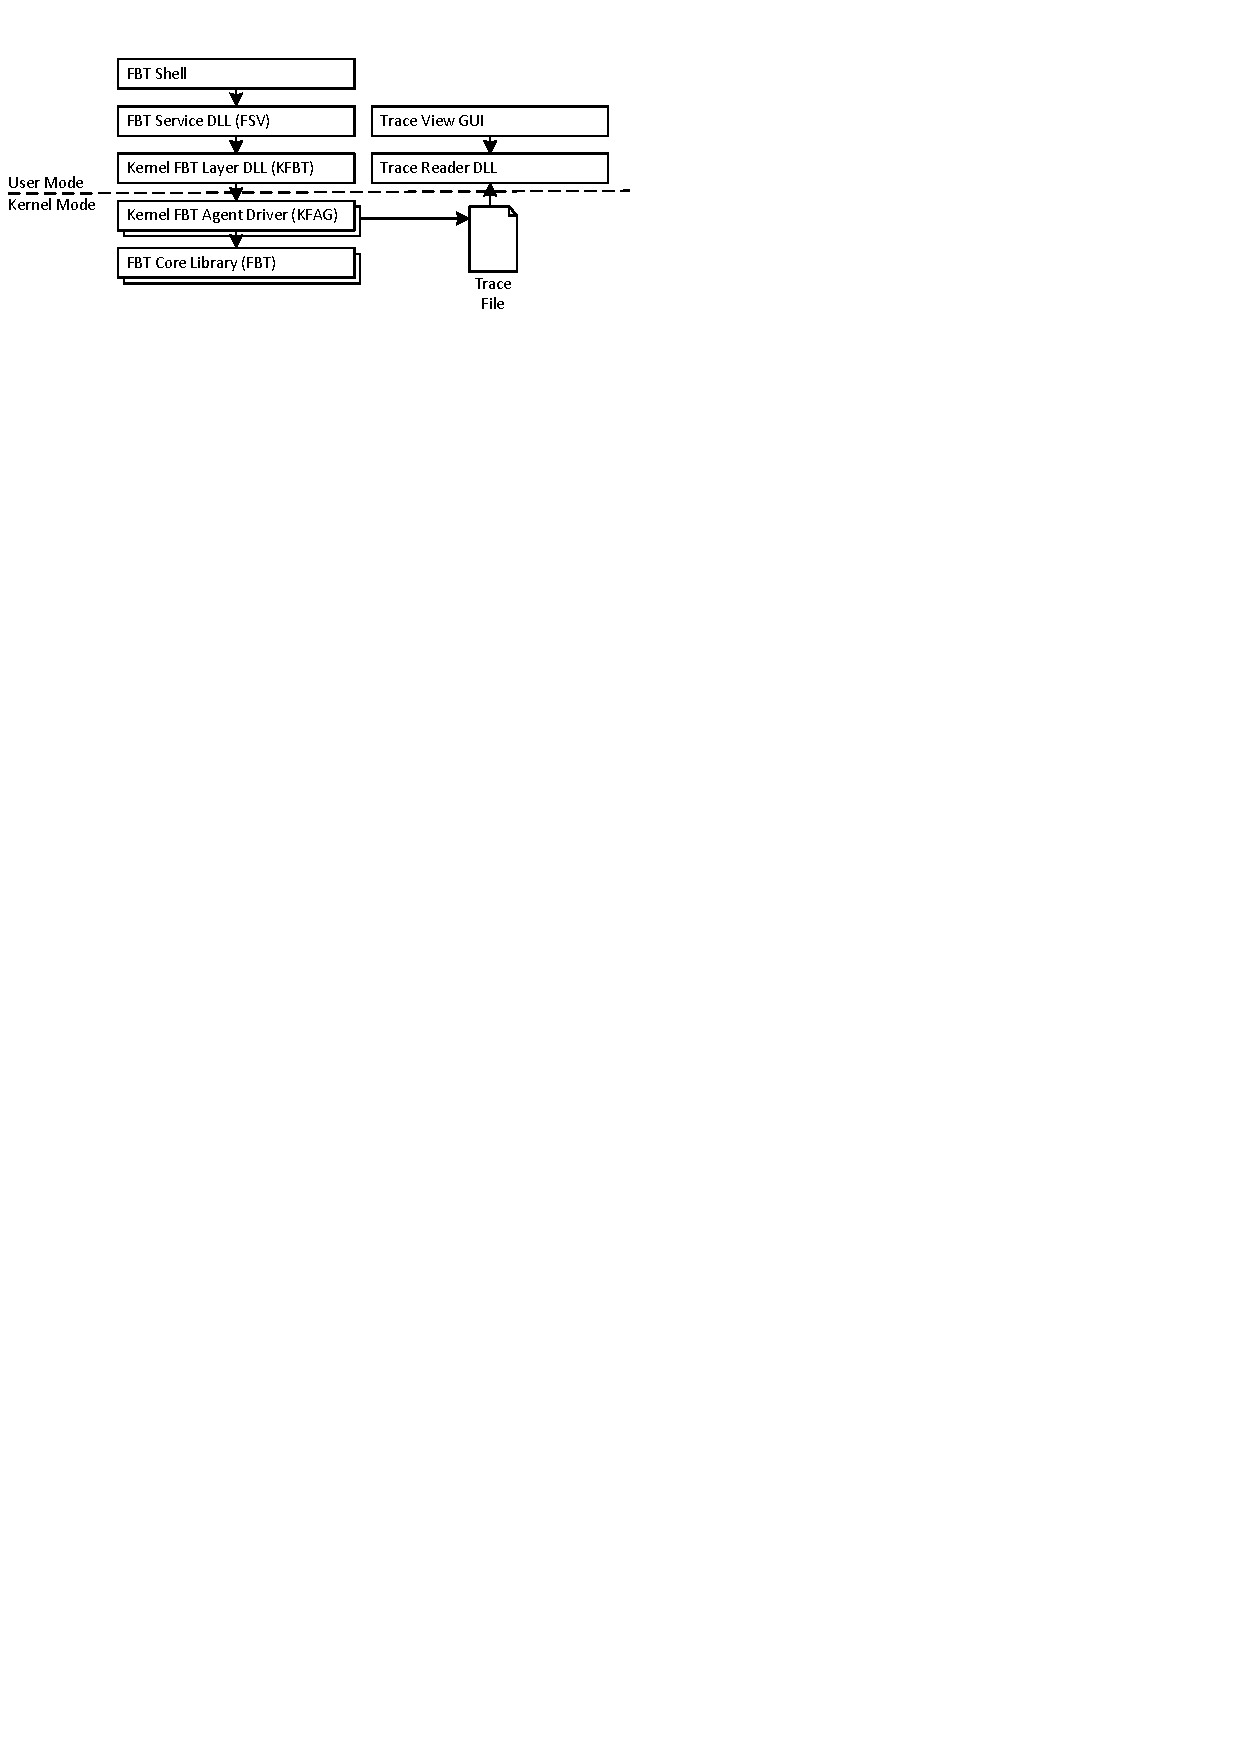
\includegraphics[scale=1, clip=true, viewport=0cm 24cm 11cm 30cm]{images/diagrams/Architecture.pdf} 
\caption{Buffer Management Dynamics} 
\label{Architecture} 
\end{centering} 
\end{figure}

The actual tracing mechanics have been implemented as a static library,
the \emph{Function Boundary Tracing (FBT) Core Library}. Both a user mode and
a kernel mode version of this library have been implemented, which share most parts
of their code. Moreover, to account for certain differences in their implementation, 
two kernel versions of this library exist -- one for the \emph{Windows Research Kernel} (WRK) 
\cite{Polze06} and one for retail kernels.

The FBT Core Library performs the bulk of instrumentation and tracing, yet it is not workable
on its own -- certain aspects, such as event handling,
are not handled by this library itself. The FBT Core Library
is embedded into the \emph{FBT Agent}, which
has been implemented as a device driver. Providing an IOCTL-based interface,
this driver wraps the functionality of the FBT Core Library and implements 
event handling by maintaining a trace file events are asynchronously written to. 
Again, two editions of this driver exist -- one for the WRK and
one for retail editions of Windows.

Besides linking against different editions of the FBT Core Library, the WRK version
has additionally been augmented by the capability of working in conjunction with
the \emph{Windows Monitoring Kernel} (WMK) \cite{Schmidt08}. The WMK is an enhancement of the WRK,
specialized for the purpose of fine-grained monitoring. Besides providing the ability
to trace a variety of events including wait events, system calls and context switches, 
it provides a dedicated tracing API. This API can optionally be used by the WRK 
version of the Kernel Function Boundary Tracing Agent, provided it is 
run on a capable kernel.

The \emph{FBT Layer DLL} is a user mode component
that simplifies the usage of the IOCTL-based interface of the Agent. Moreover, it handles
selection, lazy installation and dynamic loading of the appropriate driver. This
library, as well as all kernel mode components, does not make use of symbols but 
expects the user to work with raw function virtual addresses when requesting
functions to be instrumented. All symbol handling is performed uniformly by the 
\emph{Function Boundary Tracing (FBT) Service DLL}.

The \emph{FBT Service DLL} constitutes the top level
library. Its main duties include implementing symbol management and maintaining certain
bookkeeping information such as the list of active instrumentations. 
As such, this DLL makes extensive use of dbghelp \cite{DbgHelp}, a Microsoft 
provided library for symbol management. On top of this functionality, it also implements a simple 
command interpreter.

This command interpreter is utilized by the FBT Shell, a console based application.
With the help of the FBT Service DLL, it provides a user experience similar to the
cdb/ntsd debuggers \cite{WinDbg}, although the set of available commands is strictly limited to 
tracing-related tasks. Table \ref{FbtCommands} lists a subset of the commands offered.

\begin{table}[h] 
\caption{A subset of the commands offered by the FBT shell}
\label{FbtCommands}
\centering          
\begin{tabular}{l l}    
\hline\hline 
Command & Description	\\
\hline
tc		& Revoke instrumentation on one or more routines	\\
tl		& List active \emph{tracepoints}, i.e. traced routines\\
tp		& Set one or more tracepoints. Example: \verb|tp nt!Ke*| \\
x			& Search symbol	\\
\hline
\end{tabular}
\end{table}

Finally, a separate \emph{Trace Reader} library has been implemented for reading the 
trace file, which employs a custom binary format.
Leveraging memory mapped file techniques, the aim of this library is to provide
efficient access to the trace information and to compensate for the possibility
of lost events. Based on this library, a simple GUI application, \emph{Trace View},
allows trace information to be inspected. Utilizing a Tree View control, it also visualizes
the nesting of calls.

\begin{figure}[h] 
\begin{centering} 
%  (x, y), (x, y) from lower left corner
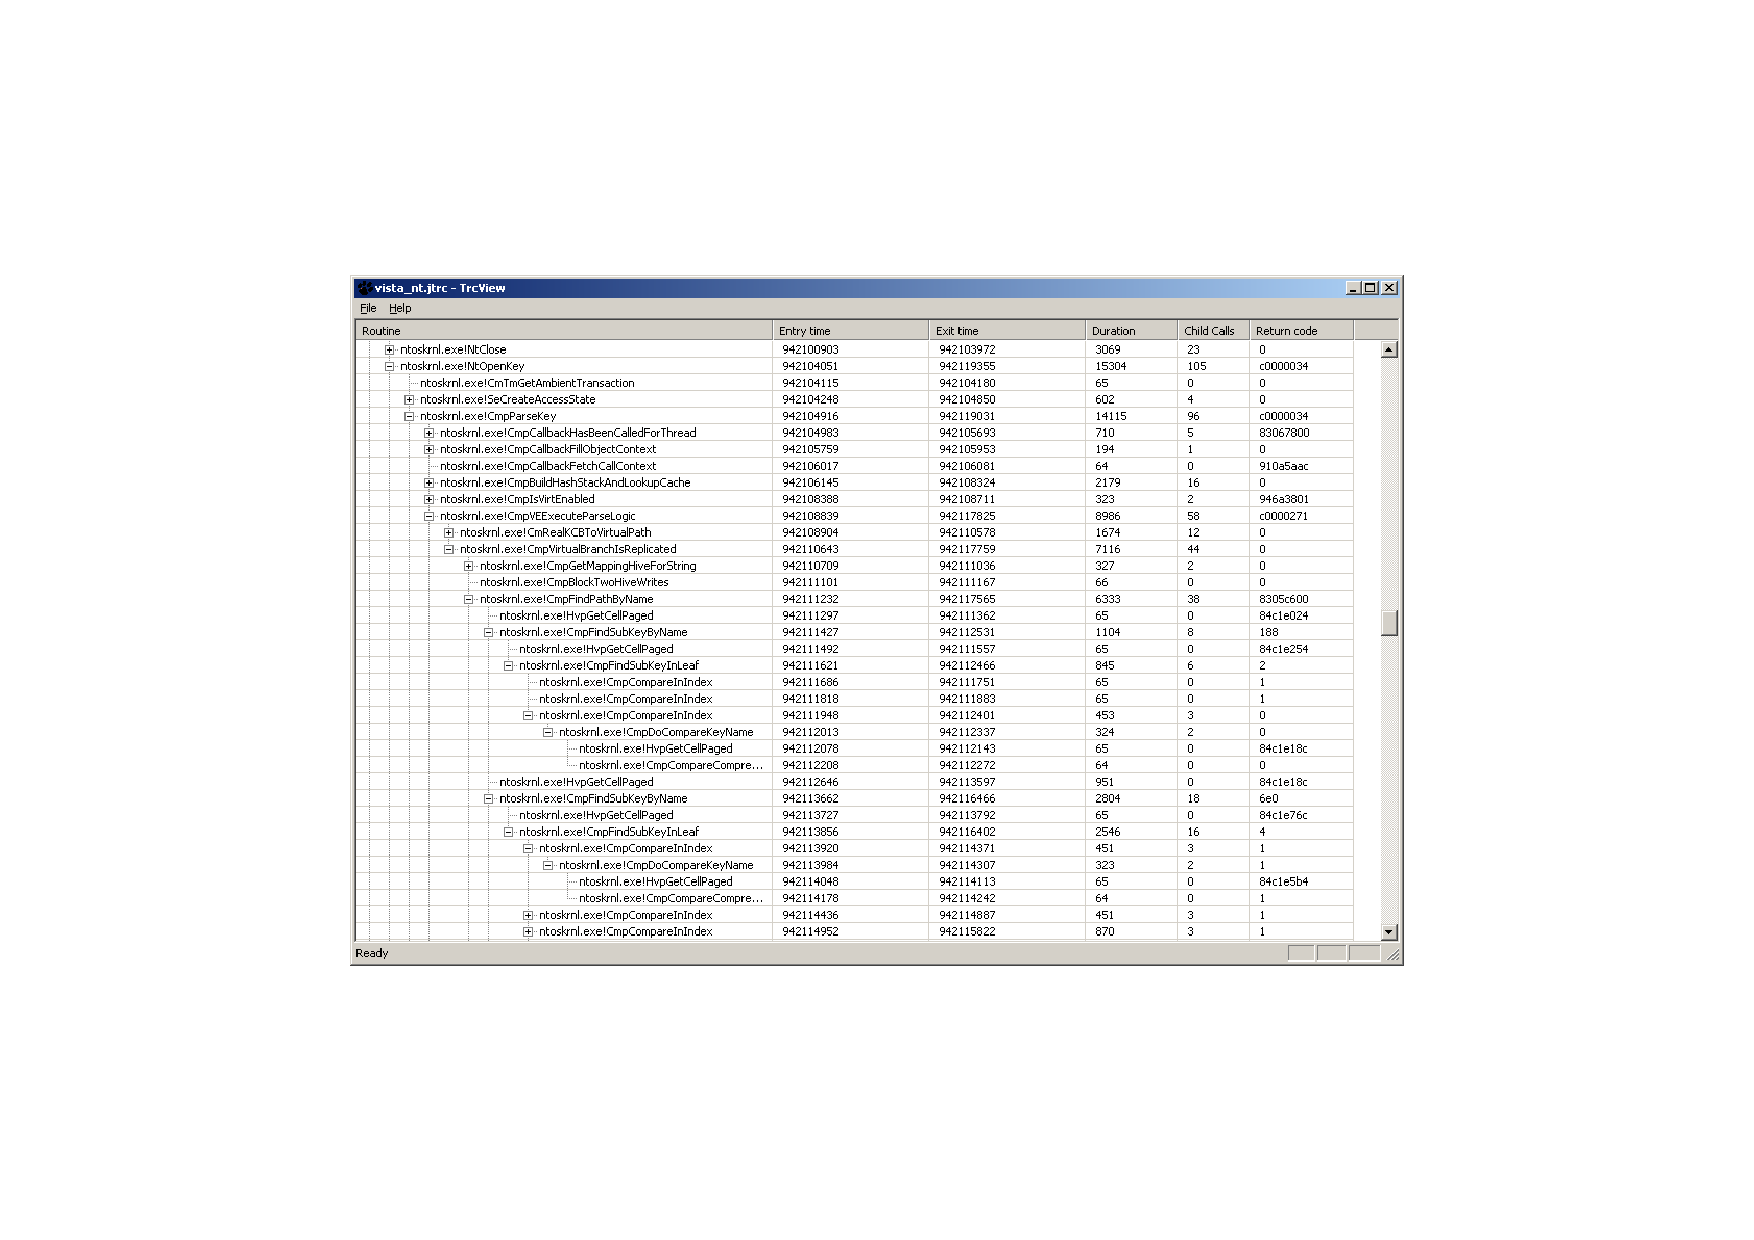
\includegraphics[scale=0.8, clip=true, viewport=5.9cm 4cm 24cm 17cm]{images/TrcViewScreenshot.pdf} 
\caption[Screenshot of the Trace View application]{Screenshot of the Trace View application, showing a trace recorded on Windows Vista} 
\label{TrcViewScreenshot} 
\end{centering} 
\end{figure}



\chapter{Approach}
\label{sec:Approach}

\section{Context}
Based on the classification work discussed in chapter \ref{sec:Classification}, 
\emph{Editing Code} has been chosen as the technique to base NTrace on. The technique
promises to be both well-suited for implementing function boundary tracing as well as allowing
tracing to be implemented in a fashion that delivers sound performance. Yet, a prerequisite 
for successfully applying this technique clearly is to properly address the runtime code 
modification concerns discussed in chapter \ref{sec:ChallengesOfRuntimeCodeModification}.

Focusing on the Windows NT platform, an important observation in this regard has been 
that to achieve safe runtime code modification, certain aspects of the Microsoft
Hotpatching Infrastructure can be leveraged. To illuminate this synergy, the respective
parts of the Hotpatching Infrastructure shall be briefly discussed.

The aim of the Hotpatching Infrastructure, which has been described and is covered by a 
patent held by Microsoft \cite{HotpPatent} is to provide a means for updating binary
modules during runtime by \emph{replacing} faulty routines by new, updated routines. 
In practice, this replacement is achieved by having old routines redirect execution to the new, 
updated routines. To install such redirections, Hotpatching, as its name suggests, employs a 
certain amount of runtime code modification.

The key aspect Hotpatching relies on in order to make such redirections safe in terms
of runtime code modification, is the notion of a \emph{hotpatchable image}. Hotpatchable
images, which have been introduced along with the Hotpatching Infrastructure in Windows
Server 2003 SP1, are characterized by being built using dedicated compiler and linker 
switches, namely \emph{/hotpatch} and \emph{/functionpadmin} respectively:

\begin{itemize}
	\item The compiler flag \emph{/hotpatch} effects the first instruction of a 
		routine to be a \verb|mov edi, edi|. This instruction is essentially a noop
		and occupies 2 bytes. These two properties -- that it does not have any
		influence on the routine's semantics and its length are crucial for
		the further discussion.
		
		For certain routines, especially for routines consisting of few instructions
		only, however, the compiler is free to neglect this switch and in fact
		does not emit said instruction. Notwithstanding this limitation, experience 
		shows that the fraction of such routines is reasonably small.
		
	\item The linker flag \emph{/functionpadmin} effects that each routine is
		preceded by a certain amount of padding. The size of the padding can be
		specified as an argument. Empirical analysis reveals that the linker usually
		fills this padding area with \verb|int 3| (opcode 0xCC) or \verb|nop| 
		(opcode 0x90) instructions.
		
		Unless stated otherwise, the remaining discussion will imply the padding size 
		to be five bytes.
\end{itemize}

While the exact mechanics of how the Hotpatching Infrastructure utilizes these
properties of hotpatchable images are only partly documented, their characteristics
will play a fundamental role in the further discussion of NTrace.

%\section{Context}
%The key idea of hotpatching as discussed so far is to create 
%redirections from old to new, updated routines. While such redirections are not 
%of interest in the context of call tracing, the infrastructure provided by Microsoft
%for these hotpatching purposes provides an interesting groundwork for the 
%implementation of a tracing solution.
%
%The most important aspect in this regard is the introduction of hotpatchable images. As
%has been discussed in the previous sections, the special characteristics of these
%images can be seen as the key for the safety of hotpatching. However, the
%use of these characteristics is not limited to creating function redirections.
%
%The key idea of the dynamic tracing solution that is to be presented is therefore to 
%combine the ideas of code editing discussed in section \ref{sec:EditingCode} with
%the new abilities offered by hotpatchable images. Based on the observation that
%hotpatchable images are in wide use already, such a tracing solution aims at
%being both widely applicable and being as safe as hotpatching.
%
%%Although the technique has been implemented both for user mode and kernel mode code,
%%only the kernel mode implementation will be discussed in this work. 


\subsection{Build Environments}
With hotpatchable images and the usage of the respective compiler and linker switches
becoming a prerequisite for successful instrumentation, it is worth regarding 
their support among current build environments in more detail. 

Although both switches have meanwhile been documented and are officially supported,
it turns out that no clear information about the availability among compiler and linker versions
seems to be currently available. A non-authorative list of compiler and linker
versions along with their capabilities with respect to these switches is shown below. 
The value \emph{(yes)} (in parentheses) means that the flags are undocumented, yet workable.

\begin{table}[ht] 
\caption{Support of /hotpatch and /functionpadmin among compiler versions}
\centering          
\begin{tabular}{l l l l l}    
\hline\hline 
Product & \emph{cl} version 	& \emph{link} version		& Supported? \\
\hline
%Visual Studio 2003							& 13.10.3077			& 7.10.3077
Visual Studio 2003 SP1					&	13.10.6030			& 7.10.6030				& (yes)	\\ 
Visual Studio 2005							& 14.00.50727.42	& 8.00.50727.42		& yes		\\
Visual Studio 2005 SP1					& 14.00.50727.762	& 8.00.50727.762	& yes		\\
\hline
DDK 3790 												& 13.10.2179			& 7.10.2179				& no		\\
DDK 3790.1830 (SP1)							& 13.10.4035			& 7.10.4035				& (yes)	\\ 
WDK 6000												& 14.00.50727.220	& 8.00.50727.220 	& yes		\\ 
\hline
\end{tabular}
\end{table}

Although their compilers support the respective switches, Visual Studio 2003 and 2005 
do not advertise the use of these features, i.e. they are not exposed to the configuration
interface and are not used by default. As a consequence, most modules built with
Visual Studio may be expected to be not hotpatchable.

For kernel mode code, which NTrace clearly focuses on, the situation is different. As of DDK 3790.1830, 
the default driver build environment (i.e. makefiles) Microsoft encourages customers
to use employs both switches. Moreover, empirical analysis of the respective modules
reveals that current kernels and drivers provided by Microsoft with Windows Server 2003 SP1 and newer releases such as
afd.sys, ntfs.sys, or tcpip.sys but also user mode libraries such as kernel32.dll and
user32.dll and even applications such as notepad.exe all have been built using the respective
compiler and linker-switches.


\subsection{Operating System Releases}
As indicated, Windows Server 2003 SP1 has been the first release to introduce hotpatchable 
images. As a consequence, the further discussion will refer to this and later releases only.

The WRK plays an another important role 
in the discussion of the proposed dynamic tracing solution. The WRK comprises 
the source code of the Microsoft Windows XP x64/Server 2003 SP1 
kernel\footnote{Certain parts of the source code, most notably, the implementation of 
hotpatching, have been omitted. However, as Microsoft provides
binary objects for these parts, it is still possible to build the kernel.}
 and has been made available for academic purposes. As such,
the WRK not only allows study of the kernel sources, it also allows 
modifications to be applied and customized kernel images to be built.

Initially, the applicability of the tracing solution was limited to a customized
version of the WRK that included a small number of code changes. By applying
certain modifications, however, it was possible to port the entire system
to the retail versions of Windows Server 2003 SP1/SP2 and Windows Vista. Still,
the availability of source code simplified the development.

Regarding the build settings of the WRK, it is worth pointing out that they do not
seem to fully reflect the build settings used by the retail kernel. Although
the /functionpadmin:5 linker switch is used during building, the /hotpatch switch is
not. As a consequence, a WRK kernel built with the default settings will not be 
hotpatchable. This stands in contrast to the retail kernel, which
seems to have been built with both respective switches used as it is in fact 
largely hotpatchable. However, this limitation of the WRK is easily overcome 
by adding the /hotpatch switch in the appropriate makefile and rebuilding the kernel.




\subsection{Symbol Management}
Not only targeting the WRK itself but also the retail kernel and drivers has another
implication on symbol management. 

An essential requirement for a dynamic tracing solution is to be able to locate
routines within a loaded binary. As the code itself does not provide sufficient
information to accomplish this, additional sources of information have to be used. The
two major sources of such information are \emph{map files} and \emph{debugging symbols},
both of which can be generated during the build of a module. Map files are not well
suited for automatic consumption, so the discussion will focus on debugging symbols,
which are specially tailored to this purpose.

The current debugging infrastructure on Windows requires compilers not to embed this debugging 
information into the module itself but store it in a separate file, the \emph{program database} (PDB).
If a PDB contains the entire set of debugging symbols, which is the default, it is said 
to provide \emph{private symbols}. For the binaries of Windows and other applications,
Microsoft does not provide private symbols but rather a stripped-down version of PDB files
only, which are said to provide \emph{public symbols}. Public symbols lack most of the
detail information provided by private symbols.

With regard to functions, private symbols include very detailed information such as 
name, offset, parameter information and calling convention. In contrast, public 
symbols merely provide the name and the offset. Moreover, distinguishing between 
functions and global variable names is not possible any more.

While a tracing solution targeting the WRK exclusively could in fact rely on private
debugging information, this requirement is prohibitive when targeting retail editions
of the kernel and drivers. Therefore, one requirement for NTrace was to restrict
symbol usage to public symbols.

\section{Operation}
\label{sec:ApproachOperation}

Having discussed the context, the basic operation of the function boundary tracing
approach implemented can now be described. The following sections provide a walk through
of how trace events are captured and consumed. Yet, most implementation details will be 
ignored at this stage and will be discussed in chapter \ref{sec:Implementation}.

\subsection{Function Entry Tracing}
Function boundary tracing includes both tracing entry and exit of a given function. Yet,
being able to trace function entry is the more basic requirement of the two and 
shall be discussed first.

To leverage the properties of hotpatchable images, the basic functionality of function
entry tracing is similar to the idea of hotpatching discussed before. To illustrate
this functionality, Figure \ref{EntryTracingSketch} shows an example of a function
\verb|Foo| that is to be traced:

Execution reaches \verb|Foo| (1), which has been instrumented before. Part of this
instrumentation is that the first instruction, which has to be a \verb|mov edi, edi|,
has been replaced with a branch to \verb|Foo-5|. Following this jump (2), execution
reaches the padding area mentioned before which precedes every hotpatchable routine.
This area has been initialized with a trampoline, which basically comprises a
single instruction that directs execution (3) to a special routine (tentatively named
\verb|CaptureEntryEvent|) which traces the call. This
routine is part of the tracing framework. After the tracing information has been obtained,
execution is redirected back (4) to \verb|Foo|. Yet, to avoid an infinite loop, 
execution continues at the second instruction, i.e. the instruction following
the \verb|mov edi, edi| (which has meanwhile been replaced by the branch instruction).
Following on, \verb|Foo| completes as normal and will finally return to the caller (5).

	
\begin{figure}[htbp] 
\begin{centering} 
%  (x, y), (x, y) from lower left corner
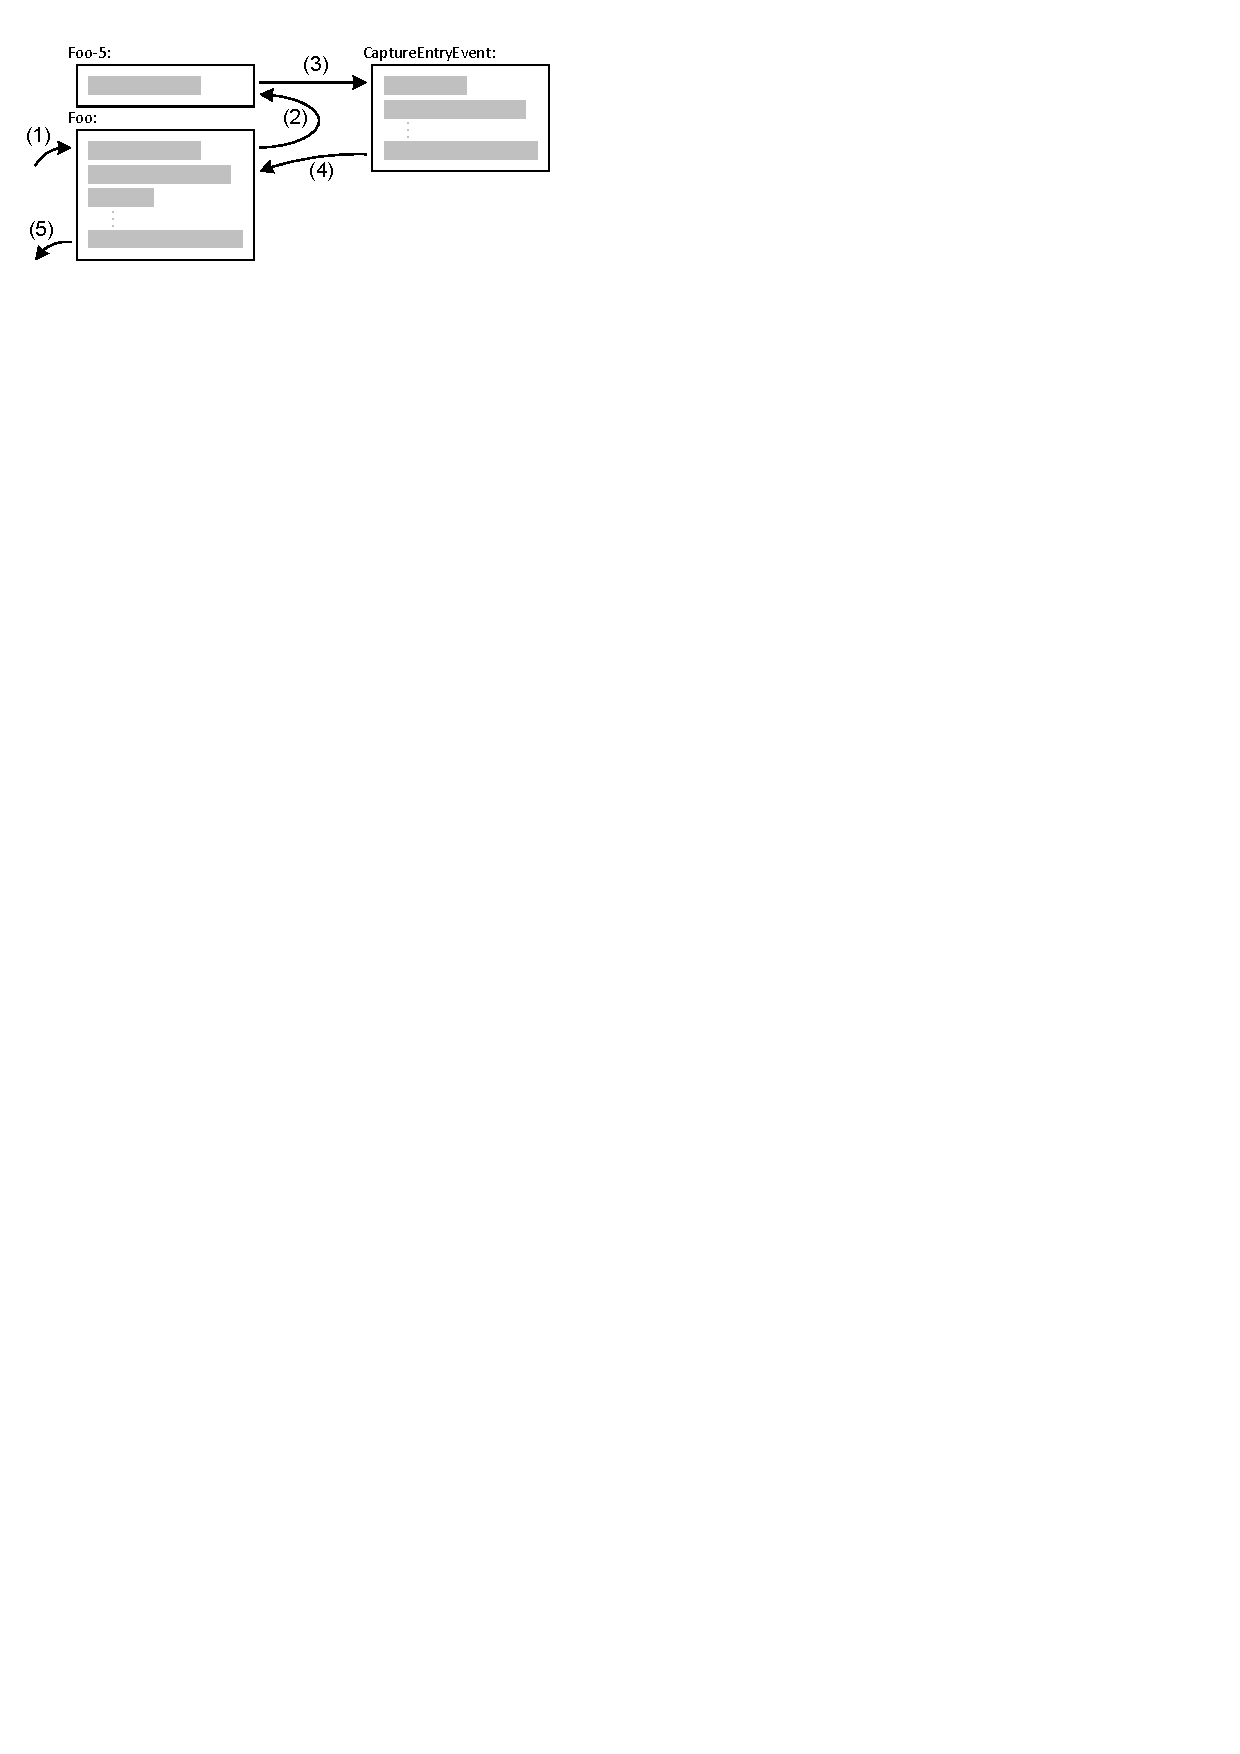
\includegraphics[scale=1, clip=true, viewport=0cm 25cm 10cm 30cm]{images/diagrams/EntryTracingSketch.pdf} 
\caption{Schematic execution flow for tracing entry events of a function Foo} 
\label{EntryTracingSketch} 
\end{centering} 
\end{figure}
	
\subsection{Function Exit Tracing}
\label{sec:FunctionExitTracing}
As discussed so far, only function entry events can be captured. To trace function exit,
the tracing solution has to regain control before the traced routine will return
to the caller.

To implement this regain of control, the function's return address is modified.
This idea corresponds to what has been described before by Brown \cite{Brown99_2} 
in the discussion of the COM Universal Delegator.

The return address of the traced function, located on the stack, contains the address within
the calling routine at which execution is to be resumed after return from the 
function. As such, it points to the instruction following the call instruction 
that led to the execution of the respective function. The layout of a stack frame
during the execution of a routine is illustrated in figure \ref{SampleStackFrame}.
In accordance to the IA-32 architecture, the stack is drawn as growing from top
to bottom.

\begin{figure}[htbp] 
\begin{centering} 
%  (x, y), (x, y) from lower left corner
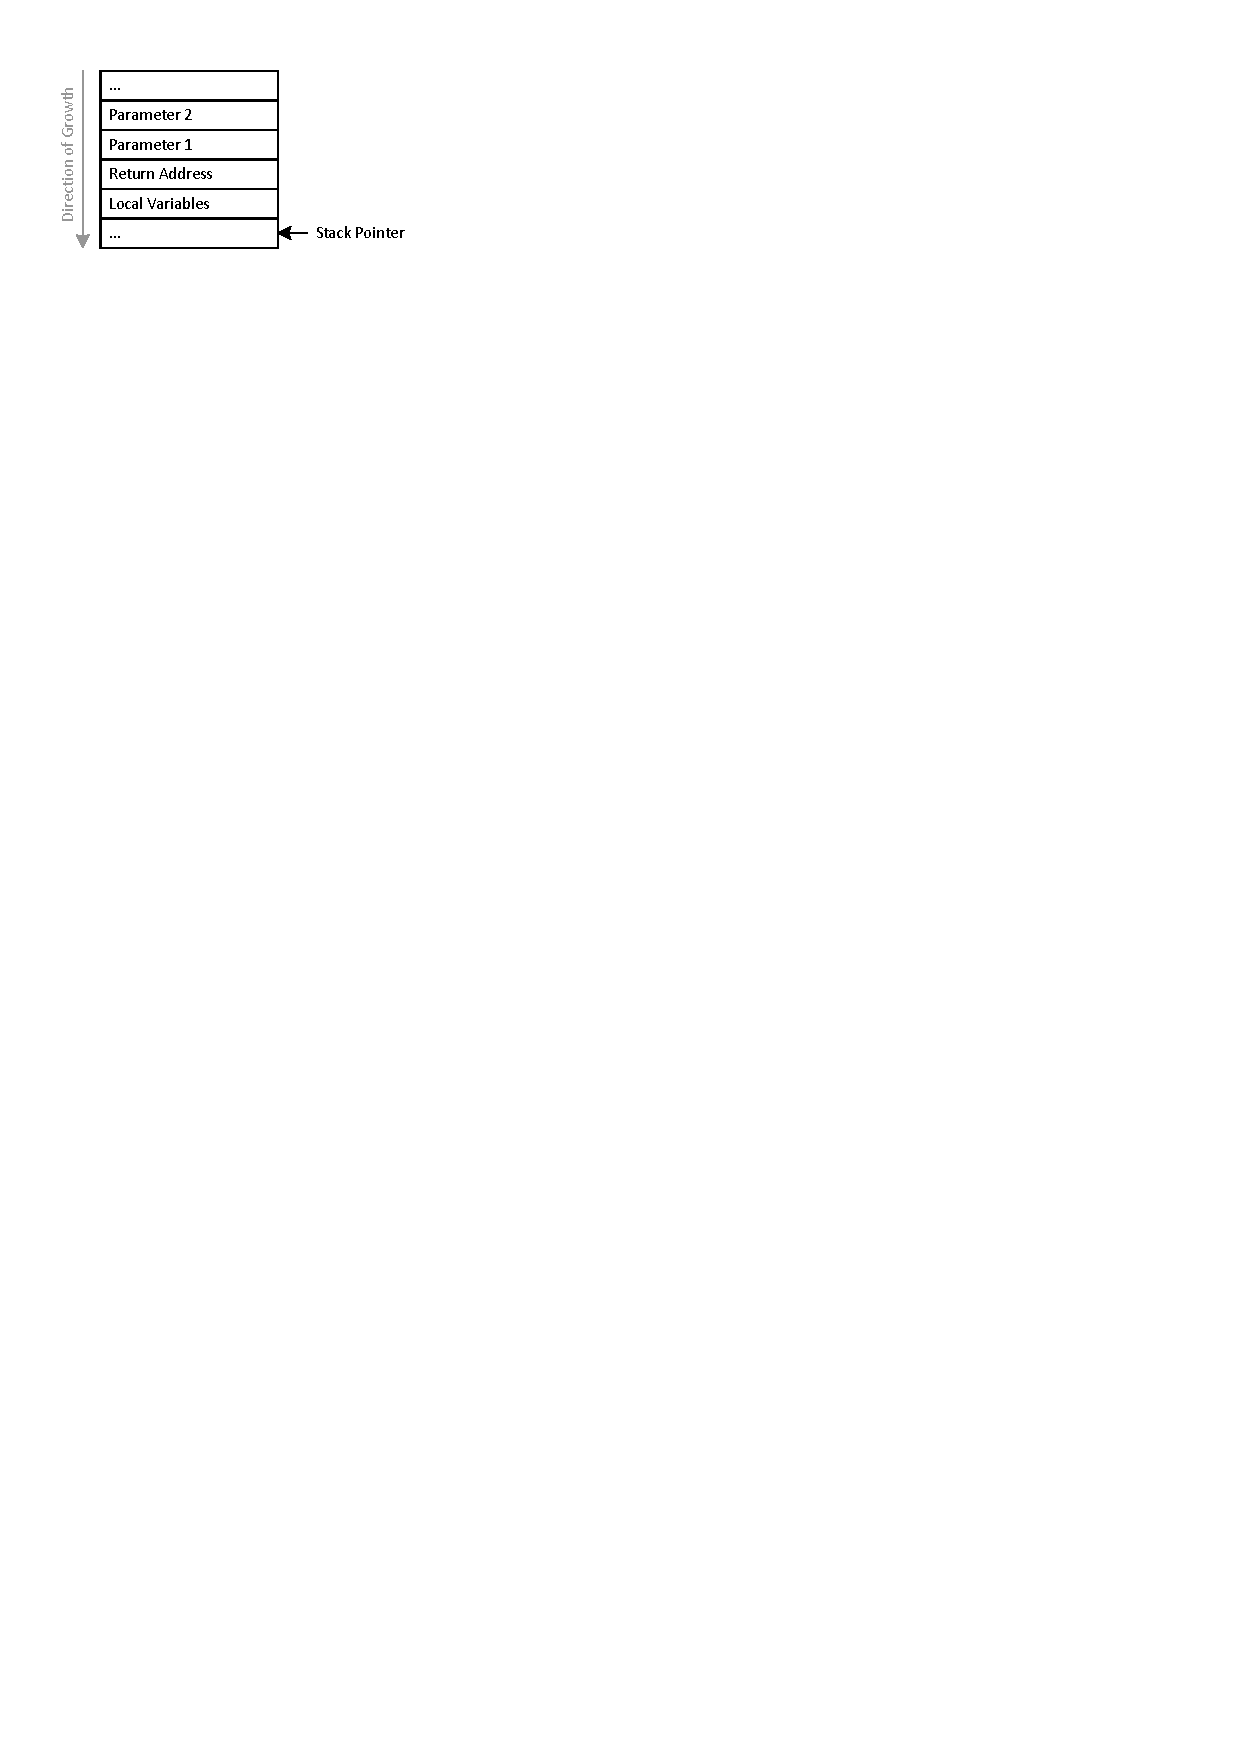
\includegraphics[scale=1, clip=true, viewport=0cm 25cm 7cm 30cm]{images/diagrams/StackFrame.pdf} 
\caption{Layout of the stack during execution of a routine.} 
\label{SampleStackFrame} 
\end{centering} 
\end{figure}

Clearly, replacing the return address is a way to regain control after the traced function
has returned. However, this technique raises two questions. On the one hand, replacing
this address is not possible before the call has been initiated and the address has been
pushed onto the stack. However, the function entry tracing technique discussed in
the previous section, already provides a solution to this issue: As this code runs after the call 
instruction pointing to the traced routine has been executed, the return
address is available on the stack and can be modified appropriately.

On the other hand, the question of how to preserve the original return address remains
to be solved. Preserving this address for the duration of executing the traced function
is crucial as this address is the only piece of information indicating where 
execution is to resume after completion of post-processing activities.

The storage location of the original return address not only has to be thread-local 
in order to be able to trace concurrently. It also has to be specific to a stack frame
in order to allow tracing recursive functions or multiple functions that call each other.

The ideal place for storing the original return address would thus be the stack itself -- the
stack is thread-local and would also nicely allow storing the return addresses in case
of recursion. Unfortunately however, usage of the stack is not possible: Pushing the 
address onto the stack during function entry would shift the location of local variables
one machine word down the stack. While this in itself may be harmless, the offset from the
stack pointer (and base pointer, if used) to the parameters increases by one machine word
as well. This increase, however, will wreak havoc on the proper operation of the routine.
As the assumptions about the relative location of its parameters on the stack will 
now be wrong, the outcome of this routine will be undefined.

To overcome this problem, the entire block of parameters could be replicated. That is,
after pushing information such as the original return address onto the stack, all parameters
are pushed again. This additional call frame would then have to be torn down during function
exit processing. However, this approach requires knowledge about the number of parameters
the individual function takes. Yet, with the restriction on public symbols, this information
is not available, which in turn makes this approach infeasible.

The route chosen is thus to provide a separate, thread-local \emph{auxiliary stack} 
for the storage of these return addresses. The implementation of this stack will be discussed in more 
detail in section \ref{sec:AuxiliaryStack}. 

\subsection{Event Callbacks}
Being able to gain control before function entry and after function exit puts the
tracing solution into the situation where it is able to produce and trace 
appropriate events.

A variety of different approaches for handling such events exist. Yet, in order
to keep the core tracing implementation free of a specific choice in this regard,
event handling is left to other parts of the system. As a consequence, 
the core implementation restricts itself to calling an appropriate entry or exit callback
routine that has been installed for this purpose before. This callback routine is provided
not only the address of the routine that is currently being traced but also
a snapshot of the general purpose register contents. It is left to
the implementation of this callback how to make use of this information.

\subsection{Putting the Pieces Together}
Having discussed the basic ideas of both function entry and exit tracing, these
techniques can now be combined. Figure \ref{EntryExitTracingSketch} illustrates
the schematic execution flow.

\begin{figure}[htbp] 
\begin{centering} 
%  (x, y), (x, y) from lower left corner
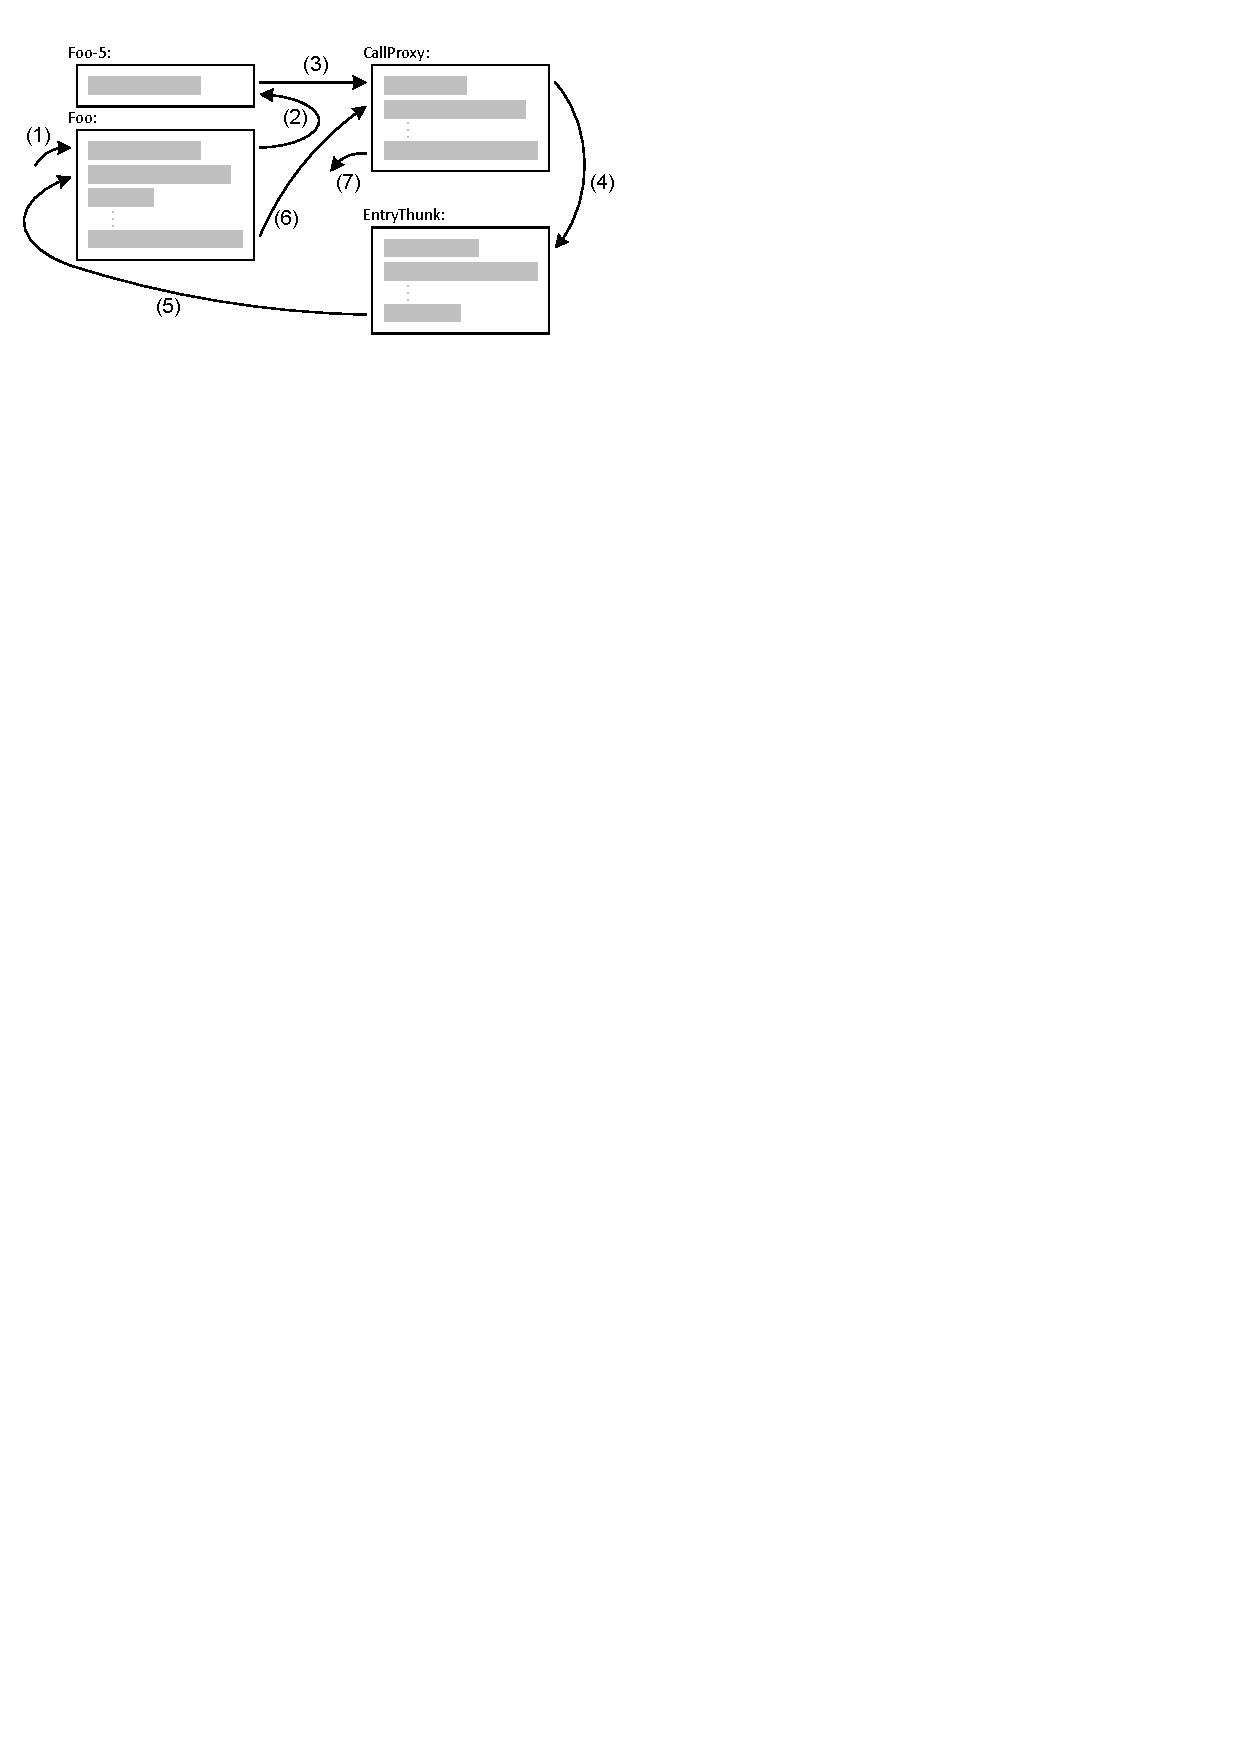
\includegraphics[scale=1, clip=true, viewport=0cm 24cm 11cm 30cm]{images/diagrams/EntryExitTracingSketch.pdf} 
\caption{Schematic execution flow for tracing function Foo} 
\label{EntryExitTracingSketch} 
\end{centering} 
\end{figure}

As a result of instrumenting the function \verb|Foo|, the \verb|mov edi, edi| instruction,
which is always the very first instruction of a hotpatchable routine, has been 
replaced with a jump to the padding area preceding the function. This padding area, 
as mentioned before, is used as a trampoline.

Using the padding area for storing the trampoline has two benefits. 
First, no memory has to be allocated dynamically and the lifecycle issues
described in section \ref{sec:LifecycleManagement} are avoided. Clearly, 
this benefit is bought in exchange for increased module size. 

The main advantage lies in the fact that the distance between trampoline 
and original routine is fixed and always 5 bytes in size. This in turn
allows a short jump to be used to redirect execution from the original 
routine to the trampoline. A short jump occupies only two bytes and is
the smallest jump instruction offered by the IA-32 instruction set. This
also explains the role of the \verb|mov edi, edi| instruction -- also being 
2 bytes in size, the mere role of this instruction is to reserve space for 
placing said jump. Although this instruction introduces a certain
runtime overhead for each routine, the performance impact can be expected
to be negligible in most cases.

It is worth pointing out that as only the initial \verb|mov edi, edi| instruction 
is replaced and this instruction has been irrelevant to the semantics of the routine, 
it is, after patching, still possible to use the routine without being redirected: 
By skipping the first instruction, the routine can still be executed and will 
yield the same results as before the redirection has been installed. 

Setting up the trampoline is not exposed to the issues of runtime code 
modification as the code being replaced is essentially dead -- assuming proper
operation, execution should never reach the padding area. Therefore, the only
critical runtime code modification is the swapping of the \verb|mov edi, edi|
instruction with the short jump.

Not requiring multiple instructions to be patched, this approach is neither exposed
to the problems of preemption and interruption (section \ref{sec:PreemptionAndInterruption})
nor to basic block boundary-related issues (section \ref{sec:BasicBlockBoundaries}).

Moreover, no true disassembly is required by this approach -- only the presence
of padding area and the \verb|mov edi, edi| instruction may need to be verified. 
Both can be implemented by a simple memory comparison.

Having entered \verb|Foo| (1) and taken the short jump, execution reaches the 
trampoline (2). Once the trampoline has been reached, two things have to happen. On the
one hand, execution has to be redirected to \verb|CallProxy|, which will initiate the 
preprocessing of the call. Having five bytes (the size of the padding area) at 
disposition, using a branch instruction supporting distances large enough to reach this
routine directly is feasible.

While the trampoline is specific to the function \verb|Foo|, the routines 
\verb|CallProxy| and \verb|EntryThunk| are not. In order to share code, all
routines that are currently in the state of being traced use these routines. Yet,
as call pre- and postprocessing requires knowledge about which routine call is currently 
being processed, these functions have to be provided the address of the traced
routine -- which, in this case, is \verb|Foo|.

As an additional complication, it is not clear at this point whether it 
would be safe to use a register for passing this information or whether 
doing so would destroy data. Consequently, this information has to be 
passed on the stack.

As it turns out, given these requirements, placing a near call instruction into the trampoline is a perfect fit. It occupies 
five bytes, supports a sufficiently large distance and pushes the address of 
the subsequent instruction onto the stack. This address, in turn, is exactly 
the address of \verb|Foo|.

Following this call instruction (3), execution reaches \verb|CallProxy|. As its first
action, \verb|CallProxy| performs a call to \verb|EntryThunk|. This additional call
will become relevant for exit tracing. At this point,
the stack contains three return addresses -- the actual return address, the address
of \verb|Foo| and the return address of \verb|CallProxy|. This is illustrated in 
figure \ref{EntryExitTracing_StackAt4}.

\begin{figure}[htbp] 
\begin{centering} 
%  (x, y), (x, y) from lower left corner
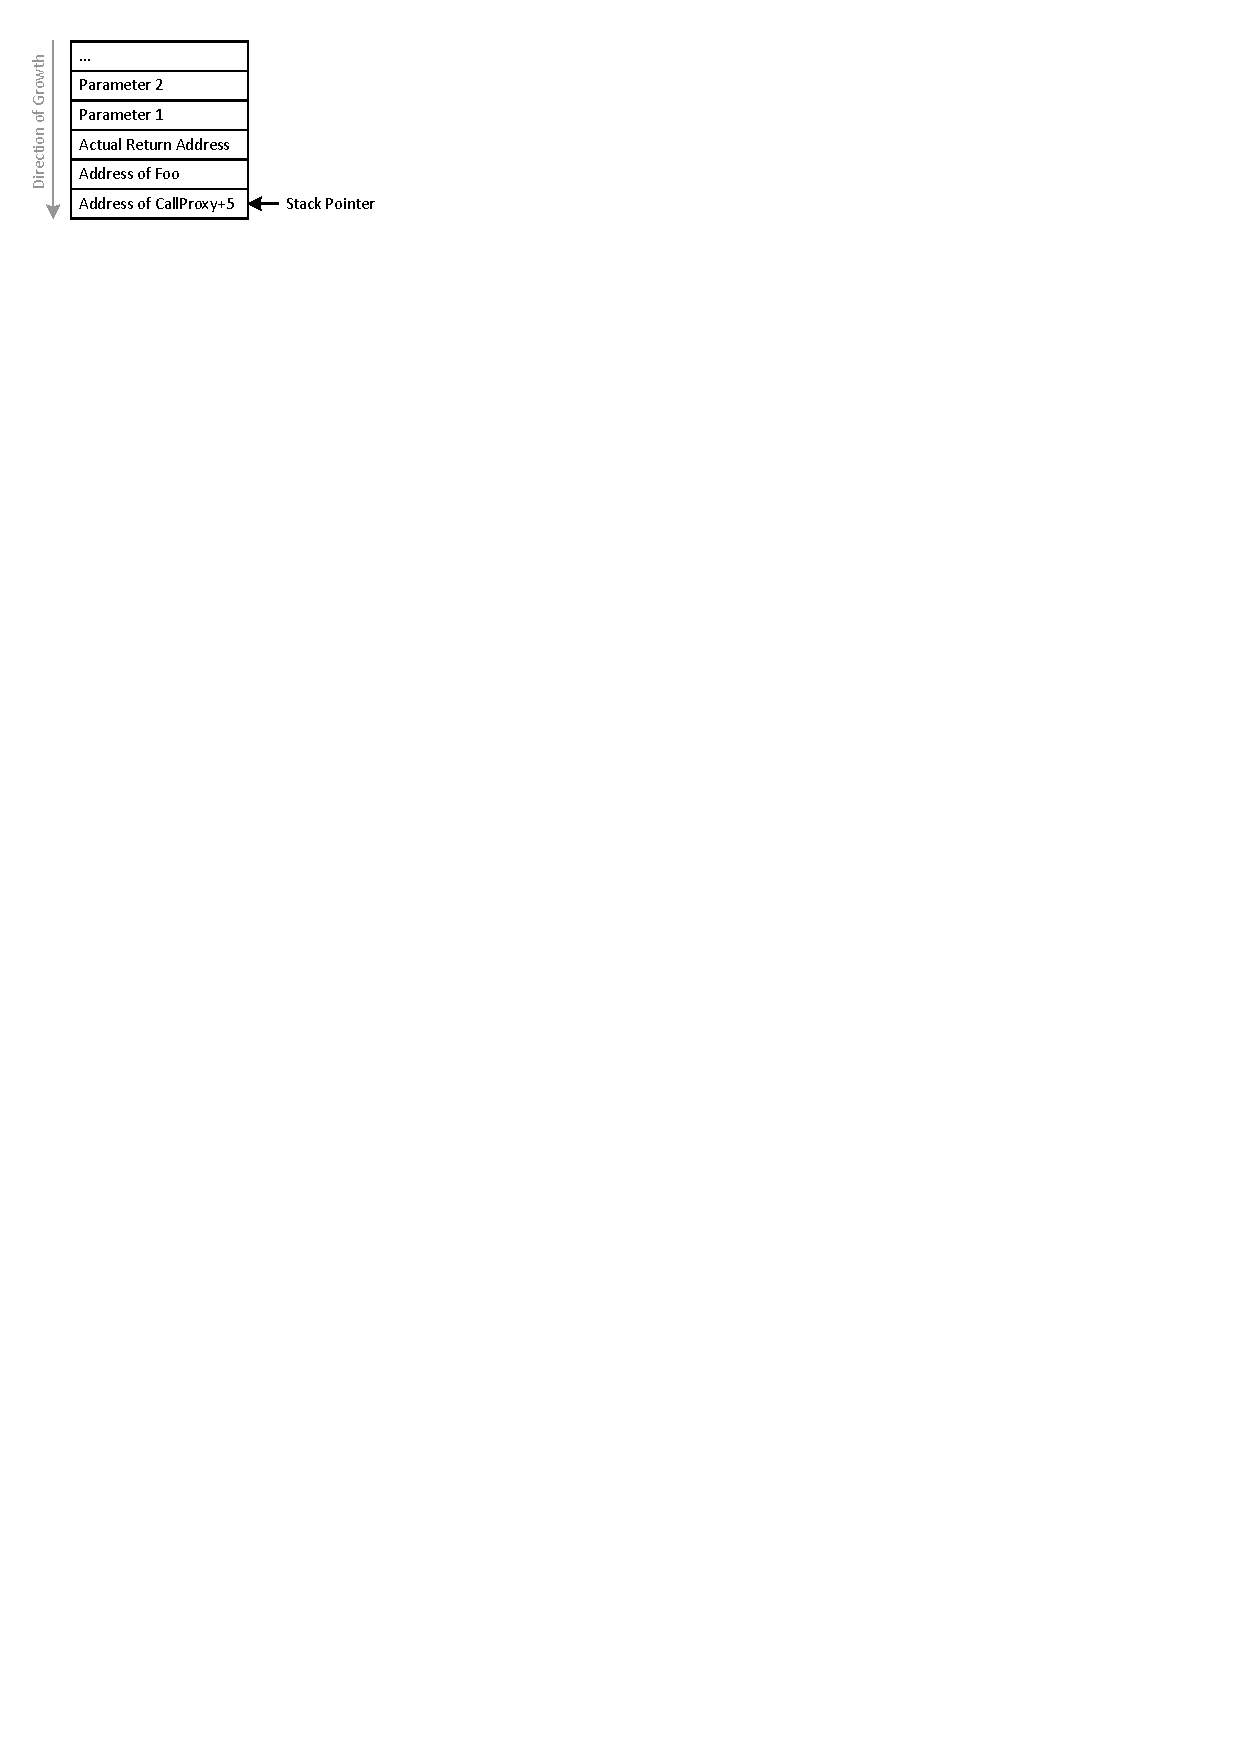
\includegraphics[scale=1, clip=true, viewport=0cm 26cm 7cm 30cm]{images/diagrams/EntryExitTracing_StackAt4.pdf} 
\caption{Stack contents at entry of CallProxy} 
\label{EntryExitTracing_StackAt4} 
\end{centering} 
\end{figure}

All three return addresses serve a specific role for the preprocessing as performed
by \verb|EntryThunk|: The actual return address, as noted before, is crucial for being
able to return to the caller after the call with all its pre- and postprocessing has 
been completed. The Address of \verb|Foo| allows \verb|EntryThunk| to distinguish
between multiple concurrently traced routines. Finally, the return address of 
\verb|EntryThunk| itself (\verb|CallProxy+5|) is required for post-processing.

\begin{figure}[htbp] 
\begin{centering} 
%  (x, y), (x, y) from lower left corner
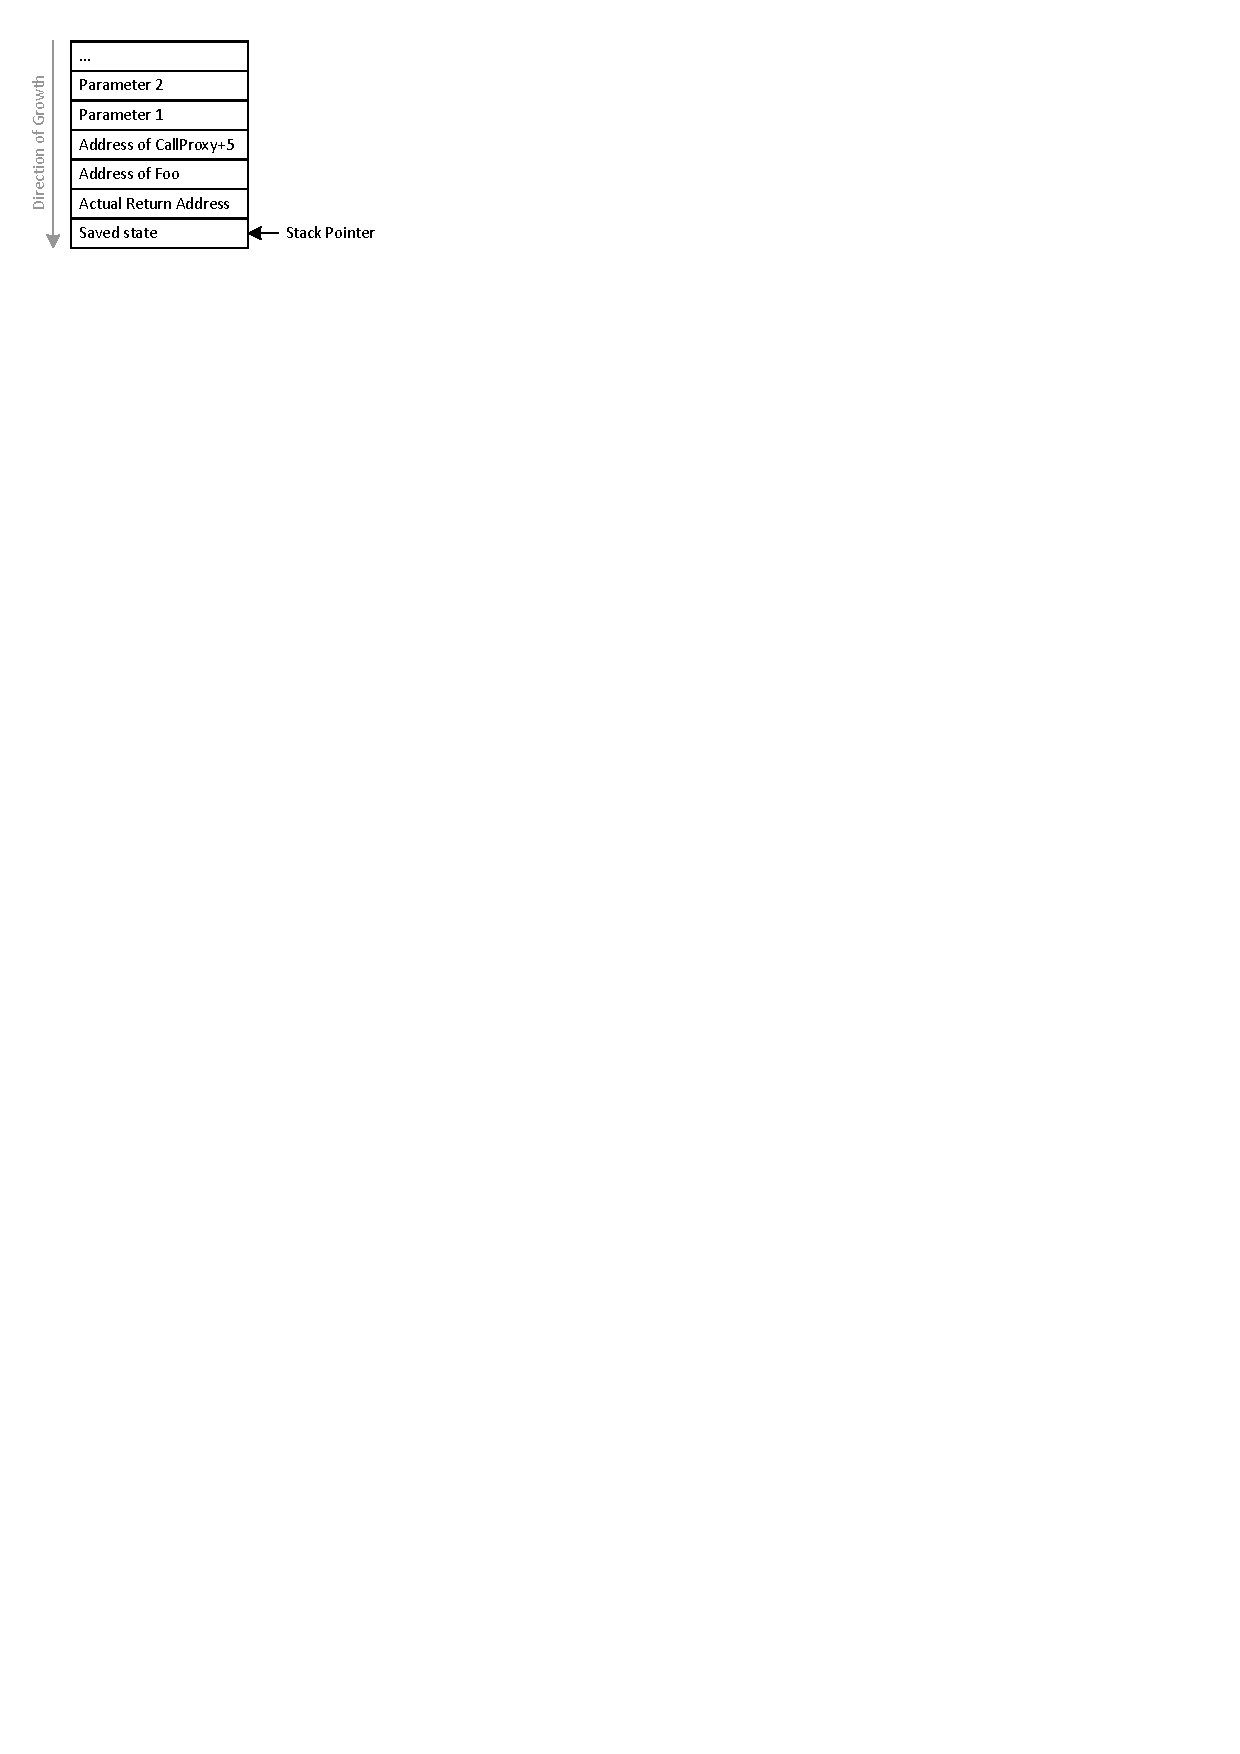
\includegraphics[scale=1, clip=true, viewport=0cm 25cm 7cm 30cm]{images/diagrams/EntryExitTracing_StackAtThunk.pdf} 
\caption{Stack contents during operation of EntryThunk} 
\label{EntryExitTracing_StackAtThunk} 
\end{centering} 
\end{figure}

Based on this setup, \verb|EntryThunk| now has the following duties:
\begin{itemize}
	\item The entry trace event has to be raised, which manifests itself in
		a callback having to be invoked.
	\item Execution has to be resumed at the called routine, \verb|Foo| (5). However,
		doing so would result in an infinite loop as the first instruction of
		\verb|Foo| is the jump into the trampoline. Therefore, execution has to
		be resumed at \verb|Foo+2|, the first instruction following this jump.
	\item Before execution can resume at \verb|Foo+2|, the stack has to be restored --
		any data that has been pushed onto the stack in addition to the single first
		return address has to be removed to ensure that \verb|Foo| -- in case it makes
		use of parameters -- is able to access these parameters properly.
	\item The single return address remaining on the stack must not be the actual
		return address but the address of the code performing post-processing, which
		is \verb|CallProxy+5|.
\end{itemize}

The steps taken by \verb|EntryThunk| are therefore as follows:

\begin{itemize}
%	\item It preserves certain register contents on the stack to make room
%		for scratch registers.
	\item The bottom-most of the three return addresses receives the return address
		of \verb|EntryThunk| itself, which is \verb|CallProxy+5|. Figure 
		\ref{EntryExitTracing_StackAtThunk} illustrates
		the state of the stack after this step has been performed.
	\item A pointer to the auxiliary stack is obtained. Both the address of the traced
		routine (\verb|Foo|) and -- most importantly -- the actual return address is
		pushed onto this stack.
	\item The function entry event is raised by invoking an appropriate callback
		routine.
	\item The stack is cleaned up. The two pieces of information that are required
		for post-processing -- function address and actual return address -- have been
		safely stored on the auxiliary stack. After trimming the stack, a return to 
		\verb|Foo+2| is performed (5), which results in execution to resume at the traced
		routine.
\end{itemize}

\verb|Foo| will eventually return in one of two ways. Either it returns normally
or it is aborted prematurely by an exception. Exception handling will be discussed 
in more detail in section \ref{sec:ExceptionHandling}.

In the usual case, \verb|Foo| will return normally and execution will resume at the
return address (6). As a result of the preprocessing, however, the return address points
to \verb|CallProxy+5| rather than to the actual calling routine. 

Having reached \verb|CallProxy+5|, postprocessing takes place. Two basic tasks have
to be accomplished:

\begin{itemize}
	\item The exit trace event has to be raised, which manifests itself in
		a callback having to be invoked.
	\item Execution has to resume at the actual caller.
\end{itemize}

To perform these tasks, the original return address as well as the address of
the traced routine is required. Moreover, such processing requires a certain amount
of stack space. 
Neither of these two addresses is reflected by the stack in its current state. 
Worse yet, as the calling convention used by \verb|Foo| is unknown, it is not clear 
either what information can still be expected on the stack and which data the stack 
pointer points to. This is illustrated by figure \ref{EntryExitTracing_StackAt6}.

\begin{figure}[htbp] 
\begin{centering} 
%  (x, y), (x, y) from lower left corner
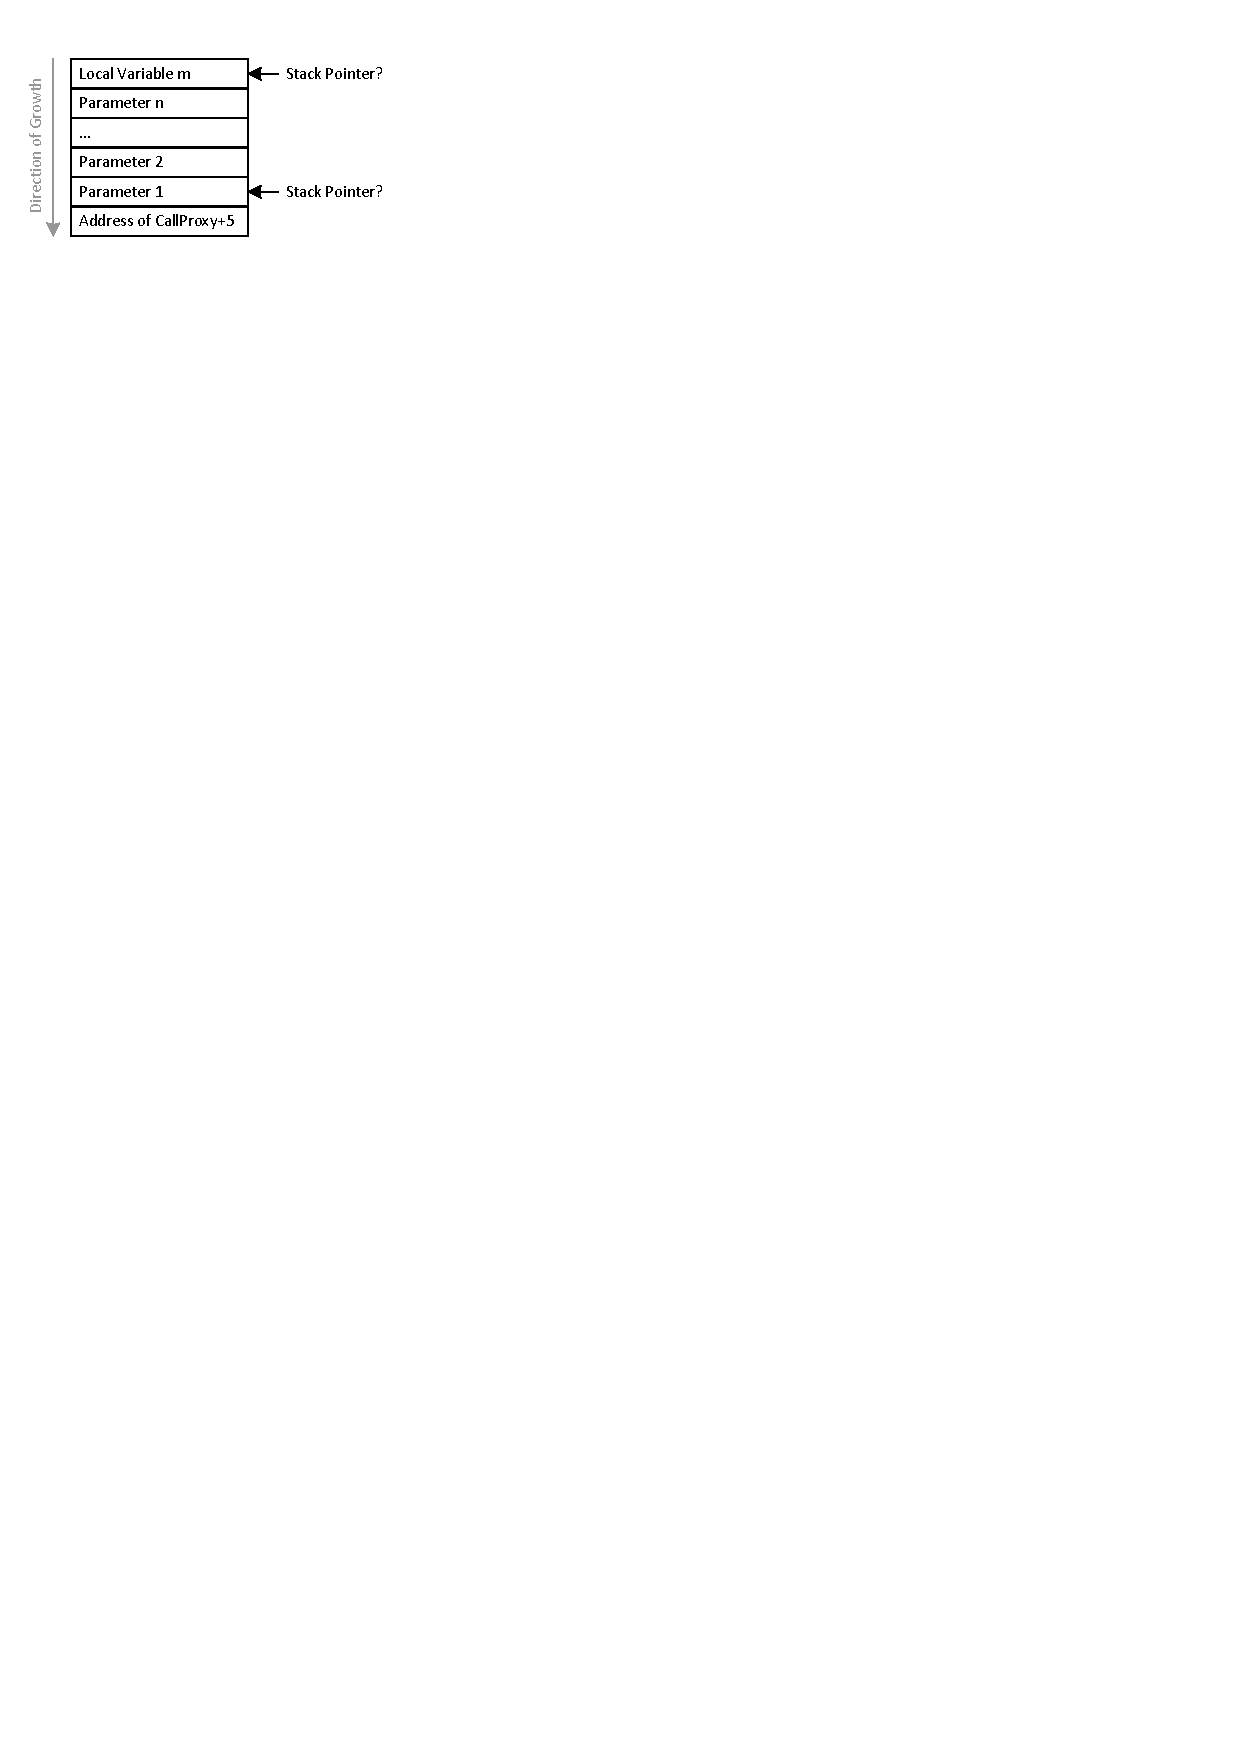
\includegraphics[scale=1, clip=true, viewport=0cm 25cm 7cm 30cm]{images/diagrams/EntryExitTracing_StackAt6.pdf} 
\caption{Stack contents after return from Foo} 
\label{EntryExitTracing_StackAt6} 
\end{centering} 
\end{figure}

Two situations may have occurred:
\begin{itemize}
	\item The stack has not been cleaned yet. The callee (i.e. \verb|Foo|) may have used
		the \emph{C Declare} (\emph{cdecl}) calling convention and thus returned
		without adjusting the stack pointer to account for the parameters. This situation, 
		for example, occurs when the function returned by executing a \verb|ret|.
		
		As a consequence, the stack pointer will now point to the first parameter 
		of \verb|Foo|, whose value may or may not still be intact. 
		
	\item The callee (i.e. \verb|Foo|) has already cleaned the stack. Calling conventions
		such as \emph{stdcall} require the callee to adjust the stack pointer to account
		for all parameters. As an example, this situation occurs when \verb|Foo| has 
		returned by executing a \verb|retn m| instruction with m reflecting the number of bytes
		occupied by its parameters. In this case, the stack pointer will now point to the
		topmost local variable of the actual callee.
\end{itemize}

Which of these situations has occurred is not clear. It is, however, possible
to deal gracefully with both situations. In both cases, it is safe to assume that
the memory above the stack pointer (i.e. lower addresses) may be used as scratch
space. 
%This assumption will be discussed in more detail in section \ref{???}.

Utilizing this scratch space, a pointer to the auxiliary stack can be acquired and
the function address (in this case, the address of \verb|Foo|) as well as the actual 
return address can be obtained.

Having this information at hand, the exit event can be raised by invoking the 
appropriate callback routine. After this has been accomplished, the scratch
data has to be removed from the stack and register contents have to be restored
so that stack and registers are in the same state as they were after return 
from \verb|Foo|.

Finally, execution has to be transferred to the caller. The crucial point to notice
is that regardless of which of the situations listed above has occurred -- 
\verb|CallProxy| is not in charge of cleaning the stack. Therefore, it is safe
to push the actual return address and return from \verb|CallProxy| with a simple
\verb|ret| instruction. This practice has the additional benefit of not requiring
a register or a memory location as an indirect jump would. After the return,
execution resumes at the caller as normal.

%A final remark on the usage of call and return statements is worth being made.
%The follwing list sums up the branches taken during processing of a call:
%\begin{itemize}
%	\item Call from caller to to traced routine
%	\item Jump from traced routine to trampoline
%	\item Call from trampoline to CallProxy
%	\item Call from CallProxy to EntryThunk
%	\item Return from EntryThunk to traced routine
%	\item Return from traced routine to CallProxy
%	\item Return from CallProxy to caller
%\end{itemize}
%As the list clearly points out, the number of call and return instructions
%match. Although matching these number of instructions is by no means a 
%requirement of the instruction set, it is beneficial in case the processor
%implements \emph{Return Address Prediction}. Although predictions will
%be wrong for the listed calls/returns due to the modifications on the
%return address, the predictor stack may be expected to remain balanced. 




	
\chapter{Implementation}
\label{sec:Implementation}

%\section{Loading}
\section{Instrumentation}
Instrumenting a routine is a multi-step process. Given the name of a single routine
or a pattern matching a set of routines, the first step is to determine 
the respective virtual addresses. This translation between symbols, i.e. routine names,
and virtual addresses requires debugging symbols. As such, it is performed
entirely in user mode by the FBT Service DLL, which in turn utilizes dbghelp 
for symbol handling. To yield valid kernel mode virtual addresses, this process
takes the current load addresses of the affected kernel modules into account. 

\subsection{Validation}
Once the virtual addresses have been obtained, the FBT Agent is sent an IOCTL command
requesting the instrumentation to be performed. It is worthwhile to notice that
the content of such IOCTLs -- the virtual addresses of routines to be implemented --
is delicate from a security standpoint. As these addresses will at least be read 
from, a malicious client could use such IOCTLs to have the kernel access invalid 
memory areas, which could in turn provoke a bugcheck.

However, such situations may even occur without malicious intent and access control by itself
is therefore insufficient to prevent such situations from occurring: A user may, for instance, accidently request
a routine to be instrumented that is part of a driver's initialization code. Such routines,
however, are commonly marked with the compiler directive 
\verb|#pragma alloc_text( INIT, RoutineName )|, which effects that the respective code
is discarded as soon as \verb|DriverEntry| has returned. Any attempt to access the
code of this routine after driver initialization has completed is likely to provoke
a bugcheck.

Thorough validation of instrumentation requests is inevitable to avoid such situations
from occurring. Yet, merely validating all memory locations before performing the actual
patching operation is insufficient to prevent damage. Memory is a shared resource and 
other threads may not only modify memory contents concurrently, but also impact the 
validity of memory at any time -- for instance, by unloading a module. Such checks
are thus exposed to a \emph{time of check to time of use} (TOCTTOU) \cite{SecAssess06} issue.

Concurrent unloading of the module to be patched can be assumed to be the most relevant
potential source of problems. In user mode windows, such problems could be mitigated
by incrementing the \emph{reference count} of the module or \emph{pinning} the module. 
Unfortunately, no similar API is provided in kernel mode Windows -- neither the 
reference count nor an appropriate lock is accessible through official APIs.

Short of such mechanisms, another approach is used: Some of the checks
are delayed until just before the actual patching operation begins. At this stage,
execution of concurrent code will be prevented and the IRQL will have been raised 
to \verb|DISPATCH_LEVEL|. As concurrent unloads are unable to take place under 
these circumstances, validation can then be safely conducted.

The entire validation logic consists of multiple steps. As a first check, the agent 
verifies that the addresses received in instrumentation requests indeed fall into 
memory areas occupied by modules. This check is still performed at \verb|PASSIVE_LEVEL|.
While this will detect attempts to access other 
memory areas such as the pool, it is yet insufficient to deal with addresses pointing 
to discarded memory or to parts of the module other than a routine. Moreover, the 
respective module could just be about to be unloaded.

%The second validation step addresses duplicate avoidance. To allow proper
%deinstrumentation at a later stage, any existing code that will be overwritten 
%during instrumentation will be copied to a central place, the \emph{patch database}. Having
%this information at hand, deinstrumentation is merely a matter of swapping the replaced
%code back in. However, a prerequisite for this pattern to work, is that any attempt 
%to instrument a routine twice must be detected and prevented as this would lead to 
%losing the original code. 

%On the one hand, 

%As a second validation step,
%duplicates within a single request must be identified. Again, this situation is more
%common than might be expected. In certain situations, such as when two routines are
%sufficiently similar, an optimizing compiler may opt to combine two routines into one,
%which in turn leads to two symbols referring to the same address. Unaware of this fact, 
%a user may chose to instrument either routine, which leads to the instrumentation request 
%containing a duplicate.

%On the other hand, duplicates w.r.t. existing instrumentations must be identified. Unlike
%any validation having occured so far, it is crucial that this step occurs while
%holding a lock on the \emph{patch database}. Without a lock, concurrent 
%instrumentations or deinstrumentations would render validation results useless. 
%This lock is kept on until instrumentation has finished and the \emph{patch database}
%has been updated.

To overcome the limitations of the first step, further validation is performed. 
However, this validation is, as indicated
before, conducted at \verb|DISPATCH_LEVEL| while preventing concurrent execution 
of other threads. That is, concurrent module unloads as well as pool allocations
are prevented from taking place.

First, the validity of memory has to be verified. In the absence of appropriate APIs 
for this purpose, \verb|MmIsAddressValid| is currently used. Despite its
name, this routine checks whether reading or writing a certain address would result in 
a page fault. In this context, an imminent page fault is an indication for the address
being invalid. Yet, in the existence of paged code, a page fault could also be harmless.
Short of being able to distinguish between these situations, any address that reading
from would incur a page fault is deemed invalid and is rejected -- false negatives
are accepted in trade for improved robustness.

Having verified the validity of memory, the instrumentability of the routines is 
verified. That is, the existence of a padding area preceding the function as well
as the first instruction being a \verb|mov edi, edi| is checked. Not before these 
checks have all been passed does the actual patching process begin.

\subsection{Applying the Patches}
\label{sec:ApplyingThePatches}
Runtime code patching, as discussed in section \ref{sec:ChallengesOfRuntimeCodeModification},
is exposed to a variety of potential problems. While some of the issues, such
as jump distance-related problems or safety concerns related to basic block boundaries
and disassembly have already been discussed or even cannot occur with the specific 
tracing approach chosen, other issues still need to be addressed.

The first issue to be discussed is memory protection. By default, The NT kernel write-protects 
images to prevent them from being modified during runtime. This write protection could
temporarily be revoked by adapting the corresponding page table entries. However, 
the NT kernel does not provide a public API for performing such modifications. 
Although accessing the page tables directly is possible, such practice would undermine
the role of the \emph{PFN Database Lock}, which in turn makes this approach risky in practice.

A different approach to attain write access to write-protected memory regions relies
on \emph{Memory Descriptor Lists} (MDLs). This approach is, as it turns out, also used internally by the hotpatching
infrastructure and has been published in \cite{Hoglund05}. The basic idea of this
approach is to \emph{lock} the respective memory region to make it resident in physical memory.
Then, an additional virtual address mapping for the physical memory backing the respective
area is created. If this second mapping permits write access, it is possible to circumvent
the protection enforced by the original mapping. Using the second mapping rather than 
the original mapping, write access is gained while relying on documented APIs only.

The actual patching operation, i.e. conducting the runtime code modification,
depicts cross modifying code. As such, the potential issues discussed in 
section \ref{sec:Atomicity} apply and have to be dealt with.

%It is, however, crucial to notice that the \emph{critical} code patch, i.e. the code
%patch being primarily exposed to the runtime code modification issues spans only
%two bytes per routine to be instrumented. Namely, the \verb|mov edi, edi|, which is
%to be replaced.

Using a simple memory move to overwrite this instruction may be considered. Yet, this 
approach is not viable as there are no guarantees about the location of the respective instruction with 
respect to memory alignment. Moreover, even when bus locking (i.e. usage of the LOCK prefix) is
used to overcome this problem, this practice would not be safe: As discussed
in section \ref{sec:Atomicity}, such practice could still lead to undefined processor
behavior. 

The route chosen by NTrace therefore is to idle all processors but the one performing
the code patch. That is, by the use of \verb|KeGenericCallDpc|, DPCs are scheduled on all
processors. Using appropriate synchronization, the execution of these DPCs is coordinated in a way
that allows one processor to conduct the runtime code modifications while all other processors
wait for the former to finish. This strategy reflects the idea of the algorithm defined
by Intel for implementing safe cross-modifying code \cite{intel07_3A}.

\verb|KeGenericCallDpc| is similar to \verb|KeInsertQueueDpc|, yet it schedules
DPCs on all processors simultaneously and additionally supplies the DPC routine with appropriate
synchronization primitives to synchronize their concurrent execution. \verb|KeGenericCallDpc|
is undocumented, yet exported by the kernel. As Hoglund and Butler have shown,
however, a similar mechanism can be also implemented based on regular DPCs \cite{Hoglund05}.

Once the DPC having been chosen to conduct the runtime code modification begins executing,
the mentioned final step of validation can be performed. As discussed before, it is crucial 
for this step to be taken while all other concurrent activity on this system has been paused.

However, at this point, it should become clear that the validation process is still
exposed to an -- albeit less severe -- TOCTTOU issue: Locking and mapping the memory 
using a MDL has to be performed below \verb|DISPATCH_LEVEL| to account for the possibility
of paged code. It is therefore not possible to perform the locking from within the DPC. 
\verb|MmProbeAndLockPages|, unfortunately, is unable to cope with all types of invalid addresses. 
Therefore, the addresses have to be checked using \verb|MmIsAddressValid| first. Yet,
due to concurrent activity, the result of the validity check may already be outdated
when \verb|MmProbeAndLockPages| is called. Given the restrictions of the API, however, 
this race condition seems hardly avoidable.

Having completed validation, each DPC raises the IRQL above all device IRQLs 
in order to protect against interrupts. Performing the actual patch then merely is 
a matter of copying memory using \verb|memcpy| -- the fact that \verb|memcpy| 
copies non-atomically is not of concern. 

When all patches have been applied, the IRQL can be lowered again, all other DPCs can be unblocked and execution
can resume on all processors. Yet, before the DPCs return, a final step is required
in order to comply with the requirements for cross modifying code \cite{intel07_3A}:
To flush all modifications, a serializing instruction, namely \verb|cpuid|, is called by each DPC routine.

To amortize the cost of the entire patching process, multiple routines
can be instrumented at once.
 
\section{Auxiliary Stack}
\label{sec:AuxiliaryStack}

%The auxiliary stack is one of the cornerstones of the tracing approach implemented. Whenever
A cornerstone of NTrace is the auxiliary stack. Whenever
an instrumented routine is entered, a stack frame will be pushed onto this stack.
During postprocessing of the routine, the frame will be popped and the information
contained is used to continue execution.

Two basic pieces of information are stored in a stack frame: The address of the routine
being executed and the original return address. As discussed in section 
\ref{sec:FunctionExitTracing}, the stack-located return address of the traced 
routine is replaced as part of the call preprocessing. Yet, 
in order to properly continue execution after return from 
the routine, the return address has to be restored during call postprocessing. For this
purpose, the address is preserved as part of this stack frame. 

The rationale of storing the routine address is less obvious. For keeping execution
flow intact, this address is not required. Rather, its sole purpose is to be included
in the event record written during call postprocessing. As will be discussed in more
detail in section \ref{sec:CallNesting}, this simplifies the consumption of events and
also allows a certain degree of compensation for lost events.

The auxiliary stack has a fixed size of 256 frames. To avoid overflows from
occurring, the entry thunk, before allocating a stack frame, checks for
this condition. In case of stack depletion, it fails gracefully by falling back
to not tracing the call: The return address and stack modifications are reverted,
so that no call postprocessing will have to take place and thus, no stack frame
is required. Execution is then redirected to the actual routine, which will execute
without being traced.

\section{Thread Data}
Containing information specific to a single thread, the auxiliary stack needs
to be maintained on a thread-local basis. However, the auxiliary stack is not
the only piece of information that needs to be kept track off for each thread.

For this reason, all thread-local state is grouped together in a single data 
structure, the \emph{Thread Data}. Each thread on which tracing activity occurs
is attached a dedicated instance of this structure.

\subsection{ETHREAD Association}
User mode Windows allows \emph{Thread Local Storage} (TLS) to be used for 
maintaining thread-local information. However, being a user mode concept,
no similar facility exists for kernel mode Windows.



TLS is maintained as part of the \emph{Process Environment Block} (PEB) and
\emph{Thread Environment Block} (TEB). Private to each thread, the TEB 
contains a plethora of thread-specific information and reserves space for 
use by TLS slots, which are defined in the PEB. PEB and TEB are maintained
by the kernel, yet they are mapped into user mode address space and can thus
be accessed from either mode. 

Although both PEB and TEB can be managed from kernel mode and utilizing TLS
from kernel mode seems feasible, it is worth pointing why this approach is
not viable.

The first obstacle lies in the fact that TLS slots are maintained on a 
per process basis. Yet, to allow TLS data to be available in an arbitrary 
process context, a TLS slot would have to be allocated for each process. To
account for the fact that slot numbers are likely to differ among processes,
a mapping between process and slot would have to be maintained as well.

But even if this problem was solved, the approach would fail to work for
system threads. System threads are used in kernel mode only and therefore
lack certain properties a user mode thread features -- which includes the
TEB. Having to implement a different approach for system threads, however, 
raises the complexity of this approach and renders it impractical.



Threads are represented by the Windows Kernel as KTHREAD structures. The 
KTHREAD structure is embedded into a ETHREAD structure, which adds additional
information used by the kernel subsystems. As such, KTHREAD/ETHREAD structures
are not only used for scheduling but also serve as thread local storage for the
kernel and its subsystems.

Drivers, however, are not offered a similar means to maintain thread local state.
Not only does the ETHREAD not reserve space for use by drivers, it is also
documented as having to be considered opaque. That is, its layout must be expected
to be subject to change.

\subsubsection{Windows Research Kernel}
On the Windows Research Kernel, this situation is easily dealt with. Having
access to the sources, the definition of ETHREAD has been enhanced by an 
additional field, \emph{PVOID ReservedForFbt}. This field is used to store
a pointer to the Thread Data structure.

\subsubsection{Retail Kernel}
Short of being able to modify the ETHREAD structure, a different strategy has
to be found for the retail edition of the Windows kernel.

Initially, a hashtable had been chosen for implementing a mapping between 
ETHREADs and Thread Data structures. Although workable, this approach had a 
number of disadvantages: As lookups can be expected to be performed
at a very high frequency -- at least once per entry or exit of a traced function --
the nature of a hashtable of offering non-constant lookup time is unfortunate.
Moreover, access to the hashtable has to be interlocked properly. Not only
must this locking be workable at any IRQL, which rules out all dispatcher-based
locks, it also has to properly guard against concurrent access by interrupts.
As a consequence, regardless of the exact locking scheme used, accessing the table
has to involve raising the IRQL. Yet, as adjusting the IRQL is a non-trivial operation,
the frequent calling of \verb|KfRaiseIrql| and \verb|KfLowerIrql| must be expected
to have a negative performance impact.

Another non-obvious drawback of the callout to \verb|KfRaiseIrql| and \verb|KfLowerIrql|
is potential interference with Driver Verifier. If Driver Verifier has been enabled for
the agent driver, \verb|KfRaiseIrql| is among the routines hooked. Unfortunately,
the surrogate implementation, \verb|VerifierKfRaiseIrql|, itself calls a number
of memory-related routines, \verb|MiTrimAllSystemPagableMemory| being one of them. If one
of these routines has previously been instrumented for tracing, this leads to endless
recursion. This situation is illustrated by the stack trace in figure 
\ref{VerifierKfRaiseIrql}, which was taken shortly before a stack overflow occurred.

\begin{lstlisting}[label={VerifierKfRaiseIrql}, caption={Stack trace illustrating recursion caused by interference of Driver Verifier with a hashtable based approach}]
[...]
nt!ViTrimAllSystemPagableMemory+0x53
nt!VerifierKfRaiseIrql+0x39
jpkfar32!JpfbtsAcquireTlsLock+0xd
jpkfar32!JpfbtGetFbtDataThread+0x11
jpkfar32!JpfbtpGetCurrentThreadDataIfAvailable+0x11 
jpkfar32!JpfbtpGetCurrentThreadData+0x11
jpkfar32!JpfbtpGetCurrentThunkStack+0xb
jpkfar32!JpfbtpFunctionEntryThunk+0x17    
   (instrumented nt!MiTrimAllSystemPagableMemory)
nt!ViTrimAllSystemPagableMemory+0x53
nt!VerifierKfRaiseIrql+0x39
jpkfar32!JpfbtsAcquireTlsLock+0xd 
jpkfar32!JpfbtGetFbtDataThread+0x11
jpkfar32!JpfbtpGetCurrentThreadDataIfAvailable+0x11
jpkfar32!JpfbtpGetCurrentThreadData+0x11 
jpkfar32!JpfbtpGetCurrentThunkStack+0xb 
jpkfar32!JpfbtpFunctionEntryThunk+0x17    
   (instrumented nt!MiTrimAllSystemPagableMemory) 
nt!ViTrimAllSystemPagableMemory+0x53
nt!VerifierKfRaiseIrql+0x39
jpkfar32!JpfbtsAcquireTlsLock+0xd 
[...]
\end{lstlisting}

In favor of a more lightweight solution that is also less prone
to reentrance, a different approach had to be taken. Ideally, the pointer
to the Thread Data structure could be stored in the ETHREAD, as in the case
of the WRK. Yet, ETHREAD does not reserve space for this and is also a
rather dense-packed structure, i.e. no spare space for storing a 
full pointer-sized value could be located.

At least two fields of the ETHREAD, \verb|SameThreadPassiveFlags| and
\verb|SameThreadApcFlags|, however, are wider than necessary. Both fields are
defined as ULONG, yet less than 16 bits are actually used. The pointer
to the Thread Data structure is thus split into two 16 bit words and each 
word is stored in the upper word of the two respective fields. The contents
of the lower words are preserved.

Both fields are explicitly documented in the WRK sources as being accessed
from the same thread only. That is, modifying the contents of these fields
can be expected to be safe without having to guard against concurrent access.
To protected against reentrance, however, it is still crucial to perform
each of the two stores in an interlocked fashion.

To account for the fact that the layout of ETHREAD evolves over operating 
releases, the offsets to the fields are chosen based on the individual
build of the kernel.

Using spare bits in the ETHREAD structure has proven to be a workable and
robust approach, yet it clearly does not quite follow good practice. However, as
has been demonstrated in case of the WRK, a similar, yet cleaner approach 
exists. Therefore, having to revert to using spare bits does not
denote an inherent limitation of the entire tracing approach but is rather
an artifact of the inability to augment the source code of the retail kernel.

\subsection{Allocation}
Being able to dynamically load and initialize the tracing system on a running
system was among the aims of the implementation. When the agent driver is first loaded,
all threads can be expected to not have a Thread Data structure attached. Yet,
before the first procedure entry event can be captured, the respective thread
must have been attached such a structure.

One option to implement timely allocation and association of Thread Data 
structures would be to eagerly attach each existing thread
on the system such a structure during initialization of the driver. Each thread
being spawned after the driver has been loaded would also have to be attached
a Thread Data structure. Despite the various race conditions this approach would
have to cope with, it also is inefficient: If only a few threads are affected by 
the instrumentation, most of the allocated structures will not be used.

Lazy allocation of Thread Data does not suffer from these problems and has thus
been favored. Not before the first procedure entry has been intercepted, is 
the structure allocated for the current thread.

However, lazy allocation introduces a different set of problems. For one, the
Thread Data has to be allocated from the non paged pool. \verb|ExAllocatePoolWithTag|,
the routine to allocate such memory, allows allocations to be made at 
IRQL \verb|DISPATCH_LEVEL| and below. It is, however, well possible that the first routine
to be traced on a thread runs at a higher IRQL -- which, for instance,
is the case for an interrupt service routine. As this is a rather common scenario, failing
the allocation under such circumstances is undesirable. To remedy this problem, 
a pool of preallocated structures is created during driver initialization,
which is used to satisfy allocation requests at elevated IRQL.

While this approach works decently when only drivers are instrumented and traced,
it becomes risky as soon as routines of the kernel image are instrumented. 

\verb|ExAllocatePoolWithTag| is a non-trivial operation and utilizes a number
of other routines. If \verb|ExAllocatePoolWithTag| itself or any of these routines
is instrumented, happens to be the first instrumented routine hit by a specific
thread, and the IRQL is below \verb|DISPATCH_LEVEL|, it will cause an allocation to be made.
Yet, calling \verb|ExAllocatePoolWithTag| to perform this allocation will cause 
the same procedure to be traced again. As there is still no Thread Data available,
an allocation will be triggered. At this stage, a point of
endless recursion has been reached, which will finally lead to a stack overflow and a bugcheck.

The initial approach to avoid allocation-related issues was to protect
against reentrant Thread Data allocations. Before \verb|ExAllocatePoolWithTag| is called,
the current thread is flagged as being in the state of allocating a Thread
Data structure. Whenever such an allocation is attempted, this flag is checked. In 
case it is set, reentrance must have occurred and the allocation request
is failed before any harm can be done. Although some events will be lost,
the danger of endless recursion is mitigated. After a Thread Data allocation has been
completed, the flag is cleared.

It is, however, worth pointing out that although being an effective 
countermeasure to reentrance, calling \verb|ExAllocatePoolWithTag| in
presence of instrumented kernel routines may still endanger system
stability: A situation that has been encountered in practice was that
one of the routines indirectly used by the background threads of the
memory manager was instrumented and happened to be the first instrumented 
routine to be hit on this specific thread. To allocate a Thread Data structure, 
\verb|ExAllocatePoolWithTag| was called. However, the special circumstances
of this call being made from one of the memory manager background threads
in the midst of their operation led to a situation where 
\verb|ExAllocatePoolWithTag| was confronted with an invalid state, 
which manifested itself in a \verb|IRQL_NOT_LESS_OR_EQUAL| bugcheck.

Taking consequences of this failure, performing lazy allocations using
\verb|ExAllocatePoolWithTag| must be expected to be too risky in this context: While
the approach can still be used in case only drivers are traced,
it should be avoided as soon as kernel routines are instrumented. Hence,
the FBT core library allows a flag to be set that causes all allocations,
regardless of the IRQL, to be satisfied using the preallocation pool.

\subsection{Deallocation}
Once the agent driver is requested to unload, one of its duties is to
clean up all resources previously allocated. Keeping track of all
Thread Data structures that have been lazily allocated before is thus
crucial in order to allow an orderly cleanup.

Before a Thread Data structure is attached to a thread, it is put 
onto a list: This list, rooted in the global structure where the agent 
maintains its state, contains all allocated Thread Data structures 
currently in use.

When the driver is unloading and it has been verified that deallocating
the structures is indeed safe, this list of Thread Data structures is
traversed. First, each structure is disassociated from the corresponding 
thread -- this is crucial to avoid leaving a stray pointer in the thread's
ETHREAD, which would lead to problems when the agent is loaded again at a later point in time. 
Depending on the pool from which it has been allocated (preallocation pool or
normal pool allocation), the structure is then freed.

Another aspect of deallocation is dealing with threads terminating before
the driver is unloaded. If such occurrences were ignored, the deallocation
logic depicted above could touch freed memory -- memory that has previously 
been occupied by an ETHREAD but has meanwhile been freed.

For this reason, the agent additionally registers for notification about
terminating threads by using \verb|PsSetCreateThreadNotifyRoutine|. Once
notified, the agent will cleanup and unregister the Thread Data structure
of the respective thread.

\section{Unloading}
\label{sec:Unloading}
Before the Function Boundary Tracing Agent Driver can be unloaded, all
outstanding instrumentation has to be revoked. For this to work, the
FBT core library maintains a list of all active code patches, the 
\emph{patch database}. Before unloading, all of these patches are revoked 
by swapping the old code, which is also preserved as part of this database, back in.
The actual code modification in conduced in the same manner as has been discussed
in the context of instrumentation.

Yet, such operation could be risky in case the affected routine is part of 
a driver rather than part of the kernel itself. In this case, it is possible
that the driver has meanwhile been unloaded, which means that the affected memory
is not valid any more. To avoid invalid memory accesses, the validity of memory
is checked once again before the code replacement is conducted.

A related, yet less common situation is where the driver has been unloaded, but the
affected memory region has meanwhile been reused for different purposes. To detect
this situation, the memory is additionally checked for containing the characteristic
jump-to-trampoline instruction.

However, merely reverting
all routines to their original state is insufficient to ensure that 
unloading the driver is safe. The following example illustrates this problem:

\begin{itemize}
	\item Thread 1 is currently executing Routine \verb|Foo|, which has been
				instrumented for tracing.
	\item Thread 2 revokes instrumentation on \verb|Foo| and unloads the
				driver.
	\item Thread 1 reaches the end of \verb|Foo| and will return into 
				the \verb|CallProxy|. As \verb|CallProxy| is part of the driver, which has 
				meanwhile been unloaded, this will result in an access violation
				or arbitrary memory contents to be executed.
\end{itemize}

The driver, being dynamically loadable and unloadable, can be considered 
dynamically allocated code. The driver code being executed as part of 
pre- and postprocessing of every traced routine is thus fully exposed
to the issues of lifecycle management discussed in section 
\ref{sec:LifecycleManagement}. As such, the situation illustrated 
merely reflects the inherent race condition already described.

As indicated by section \ref{sec:LifecycleManagement}, the best the
driver can do in such situations is to try to minimize the risk by
tracking usage of the dynamically allocated code. Although such
practice cannot remedy the problem in its entirety, delaying the unload
until the usage count has dropped to zero decreases the likelihood
of such problems significantly.

As a fortunate side effect of the tracing mechanism implemented and discussed so far, 
introducing additional reference counting to implement such usage
tracking is not necessary. Rather, the auxiliary stacks of all
threads can be checked for being empty. If any of the stacks is
non-empty, execution is delayed by one second and the check is retried.

Like reference counting, this mechanism is effective, yet still
exposed to race conditions. On the one hand, the implicit
assumption of that the auxiliary stacks cease to grow as soon as
all routines have been uninstrumented is flawed: It is possible
that when uninstrumentation occurs, some thread may already have entered
the \verb|EntryThunk|, but is preempted before being able to allocate a frame 
on the auxiliary stack. Resuming execution at a later point in time,
a stack frame allocation will be conducted although all instrumentation 
has meanwhile been revoked.

On the other hand, it is possible that the last frame on the auxiliary 
stack has been removed, yet execution has not yet left the CallProxy. 
Again, the driver code is still in use although all auxiliary stacks
may already be empty.

Unable to avoid these race conditions, the driver follows the approach
as taken by KernInst \citep{tamches99finegrained,Tamches01} and introduces a further three-second delay. During these
three seconds, all threads are given the chance to leave the critical code
sections.

Although still not entirely safe, this unloading strategy has worked
well in practice. However, especially when instrumenting large 
amounts of routines, it turns out that it may in fact take a significant 
amount of time before all traced routines have completed. It is thus not unusual
for the driver unload to take several seconds or minutes.

When instrumenting the kernel itself, this becomes even more noticeable, as
the kernel contains a number of routines that may block for significant
amounts of time. One such routine is \verb|KeWaitForSingleObject|. When used
for a wait that takes an hour to be satisfied -- possibly on behalf of a 
user mode application -- it will not return before this hour has elapsed.
If \verb|KeWaitForSingleObject| has been instrumented and the driver is
later requested to be unloaded, unloading will also be delayed until this wait
has been satisfied. 

Not before these safety checks have been passed, the driver begins to tear down.
This includes disassociating ThreadData structures from their threads and 
freeing the respective allocations, as well as flushing buffers.

\section{CallProxy and CallThunk}
The general working of the CallProxy and CallThunk routines and the way
they are used to intercept function invocation has been discussed
before in section \ref{sec:ApproachOperation}. 

However, a number of details about the implementation of these routines
have not been discussed so far.

\subsection{State Preservation}
The aim of the CallProxy and the EntryThunk is to interpose the call
to a routine. Yet, in order not to change the outcome of the call, it 
is crucial that the \emph{contract} between the calling and the called
function remains intact.

In this regard, the \emph{contract} between the two function is defined
by the calling convention. The calling convention defines in which memory
locations and in which order parameters have to be passed, where the
return value of the function is to be stored and whose duty it is to clean
up stack space that might have been occupied by parameters.

Regarding the WRK sources and the header files of the WDK, the most prominent 
calling convention encountered in the kernel is \emph{stdcall}, followed by
\emph{fastcall}, which is used rather infrequently.

One approach to ensure that the contract between two functions remains
intact could be to rely on the call adhering to a certain calling convention.
Having access to public symbols only, it is not clear which calling convention
is used. Yet, it is reasonable to assume that it is either \emph{stdcall}, 
\emph{fastcall}, \emph{cdecl} or \emph{thiscall}. Based on this assumption, 
it would, for instance, be safe to not
preserve the contents of the \verb|eax| register during call preprocessing. \verb|eax| is
volatile and none of the mentioned conventions use it to pass parameters.
In the same manner, \verb|ecx| would not need to be preserved during postprocessing.
Again, \verb|ecx| is volatile and is not used to store the return value by any
of these calling conventions.

Although appealing, this approach is not feasible in practice. For \emph{exported}
routines, i.e. routines made available for use by a different module, the compiler
indeed makes sure that the calling convention is adhered to. For routines used
internally, however, the compiler is free to ignore the specification of a calling 
convention: Rather than passing all parameters on the stack as the respective calling convention 
may specify, the compiler may, for instance, decide to pass one or more parameters 
in registers.

It is worth pointing out that not only \verb|static| routines, i.e. routines
used within a single object file only are subject to such optimization. With the advent
of link time code generation, the Microsoft compilers are capable of performing such 
interprocedural optimization on the entire image, rather than on individual objects only.
As a consequence, any routine not exported by the respective module must be assumed
to potentially not adhere to any of the default calling conventions.

Aiming at being able to trace internal routines as well as exported routines, 
this approach has thus been dismissed. Yet, for a solution that restricts itself
to intercepting exported routines such as \emph{IAT hooking}, this approach may
in fact be viable.

Short of any guarantees by the compiler, a rather pessimistic approach had to be
taken:
\begin{itemize}
	\item	Not knowing which registers are used to pass parameters, which
				registers are nonvolatile and which registers are free, the assumption is that
				all registers contents have to be preserved -- both during call pre- and 
				postprocessing.
	\item It is assumed that an arbitrary amount of stack space is used for passing
				parameters. Whether the caller or the callee is in charge of cleaning the 
				stack is unknown.
	\item All memory beyond the current stack pointer (i.e. higher addresses)
				is assumed to be unused.
\end{itemize}

The last item requires further discussion. The stack pointer points to the
topmost item on the stack. Convention dictates that stack memory 
beyond the location pointed to by the stack pointer, should not be accessed.
Still, such memory locations can be easily addressed and the compiler could 
generate code that does so.

There is, however, a simple reason why it is safe to assume that kernel 
mode code does not defy this convention: Interrupt processing. 

If an interrupt occurs and no privilege-level change has to be performed,
the CPU will push the EFLAGS, CS and EIP registers on the stack \cite{intel07_1}. That is,
the stack of whatever kernel thread happens to be currently running on this CPU is reused
and the memory locations beyond the stack pointer will be overwritten by these
three values. Handling the interrupt, which involves running the \emph{interrupt
service routine} (ISR) occurs on the same stack as well.

As a consequence, code accessing memory locations beyond the current stack pointer
would have such memory locations be overwritten in case of interruption. As
the compiler can be assumed to be unaware of which code sequences are subject
to interruption and which code sequences are not, it is safe to assume that the
compiler will always emit code that adheres to this convention. The same holds
for hand-written assembly code sequences, although these routines tend to be not
hotpatchable anyway.

The consequence of this observation is that the CallProxy and EntryThunk can
safely use the stack as scratch space as long as they adjust ESP accordingly.
Due to the restriction of having to preserve all register contents, this ability
to use the stack is essential. It allows both the CallProxy and EntryThunk to
establish a stack frame and to free a certain amount of registers by pushing
their contents onto the stack and restoring them later. 

%Finally, it is worth pointing out that preservation of the general purpose
%registers is sufficient. CallProxy and EntryThunk themselves do not make
%use of other registers. Yet, the event callback routines, which are invoked 
%may chose to use floating-point operations, MMX, 3DNOW!, or Intel's SSE extensions.
%However, Microsoft requires driver routines that intend to use the FPU to 
%explicitly save and restore the FPU state, which in turn frees CallProxy and 
%EntryThunk from having to do so.

\subsection{Reentrance}
\label{sec:ThunkReentrance}

During call pre- and postprocessing, the state of the thread-local ThreadData
structure is modified. This modification, which includes, but is not limited to
setting up a frame in the auxiliary stack, is a multi-step process. Although
being consistent at the beginning and at the end of this process, the ThreadData
structure will temporarily be inconsistent during this modification process.

This temporary inconsistence will become an issue as soon as the thread is 
interrupted while being in the midst of a ThreadData modification process. If
any routine that is being executed as part of the interrupt processing has
been instrumented for tracing, reentrance will occur. That is, the preprocessing
of the call to such a routine will operate on an inconsistent ThreadData structure,
which leads to arbitrary behavior. 

However, not only the modifications to the ThreadData structure themselves are sensitive
to reentrance. Lazy allocation of these structures is equally affected. Even when
the allocation code is fully reentrant, situations can occur where two structures
are allocated for the same thread. Management of buffers, a topic discussed
in section \ref{sec:EventManagement} is affected in a similar manner.

Properly handling reentrance is thus crucial. The two options are thus to either 
make all affected code fully reentrant or to properly guard against 
reentrance. While the first option may in fact be feasible, the affected 
routines of the current implementation only partially achieve this aim.
That is, both the CallProxy and the EntryThunk contain a window of instructions that
must be protected from reentrance.

To attain this protection, a simple scheme has been implemented. Leveraging one
of the bits borrowed from the ETHREAD, a flag has been introduced. Before
entering the critical window, the flag is attempted to be set; it is cleared as
soon as the window is left. If the flag turns out to be already set when entering
the window, reentrance must have occurred. Similar to what occurs on auxiliary
stack overflow, any modifications are reverted and the respective routine is 
executed without being traced.

It is worth pointing out that the situations depicted above do in fact occur on a
regular basis. In practice, before appropriate countermeasures had been put
in place, and all kernel routines (i.e. \verb|nt!*|) were instrumented, it was only
a matter of seconds before these problems led to a triple fault.

%\subsection{Stack Walking Interference}
%An unfortunate sideeffect of replacing the return address of a function is that it
%interferes with stack walking. Stack walking on IA-32, regardless of whether symbols 
%are used or not, relies on finding return addresses on the stack to step from
%one frame to another.
%
%STACKTRACE!


%\subsection{Dispatcher Routines}
%Using the Thread Data structure attached to the current ETHEAD both during call
%pre- and postprocessing assumes that the current ETHREAD does not change during
%execution of the traced routine. While this assumption holds for almost all
%routines, there are a number of routines where the current ETHREAD during 
%call preprocessing differs from the current ETHREAD during postprocessing: 
%dispatcher routines\footnote{Routines of the dispatcher that implement
%scheduling. Not to be confused with dispatch routines.}. 
%
%The current thread is maintained in the current processor's PCR. The dispatcher 
%includes a set of routines that potentially modify this pointer as part of
%their dispatching work. Based on an analysis of the WRK source code, these are:
%
%\begin{itemize}
%	\item KiSwapThread
%	\item KiQuantumEnd
%	\item KiIdleSchedule
%	\item KiExitDispatcher
%	\item NtYieldExecution
%\end{itemize}
%
%These routines are exempted from instrumentation and thus cannot be traced. The
%set of routines is small enough that this limitation is assumed to be
%insignificant.
%  
  
\section{Exception Handling}
\label{sec:ExceptionHandling}
Windows NT features a builtin exception handling infrastructure, 
\emph{Structured Exception Handling} (SEH). SEH exceptions are not only
used for handling \emph{software exceptions}, i.e. exception explicitly
raised via \verb|RtlRaiseException|. It is also used for handling hardware-defined
faults or traps such as \emph{Integer divide by zero} conditions.

So far, the existence of exceptions has largely been ignored in the
discussion of function entry and exit tracing. Rather, the implicit
assumption has been that for each function entry successfully intercepted,
there will be an intercepted function exit. During preprocessing, a frame is
pushed onto the auxiliary stack, during postprocessing, a frame is popped.
As entry and exit interceptions cleanly nest, it is assured that the popped
frame is in fact the right one, i.e. the frame corresponding to the specific
call frame.

Exceptions, however, thwart this assumption. When a routine raises an 
exception, the exception can cause the routine to not run to completion 
but to be left prematurely. The same holds for all routines corresponding
to the call frames between the call frame handling the exception and the
call frame raising the exception. All these routines will be left prematurely
as well. Prematurely leaving a routine means that it does not return to the
caller as normal. This, in turn, becomes a problem if one of the routine has 
been instrumented for tracing: a skipped return implies that postprocessing 
will not be able to take place and thus, that the corresponding frame will
not be popped from the auxiliary stack.

An unbalanced auxiliary stack entails three basic issues. The least of 
which is a resource leak: The un-popped frames will remain on the stack
and new frames will be pushed atop of these frames. Preventing the auxiliary
stack from ever becoming empty again, these frames effectively denote a
resource leak. Diminishing the effective size of the stack, they also raise
the probability of stack depletion. As discussed in section \ref{sec:AuxiliaryStack}, such 
auxiliary stack depletions can be properly dealt with. However, they will
still lead to more events being missed.

The second issue is an implication of the frames being leaked. As the
auxiliary stack will never empty again, the unloading logic discussed in 
section \ref{sec:Unloading} will keep identifying an affected thread as still being active: Short
of being able to distinguish leaked frames from non-leaked frames, it
will assume that the thread is still running traced routines. Waiting for
these routines to complete, however, will be unfruitful -- the unload will
take forever.

\begin{figure}[htbp] 
\begin{centering} 
%  (x, y), (x, y) from lower left corner
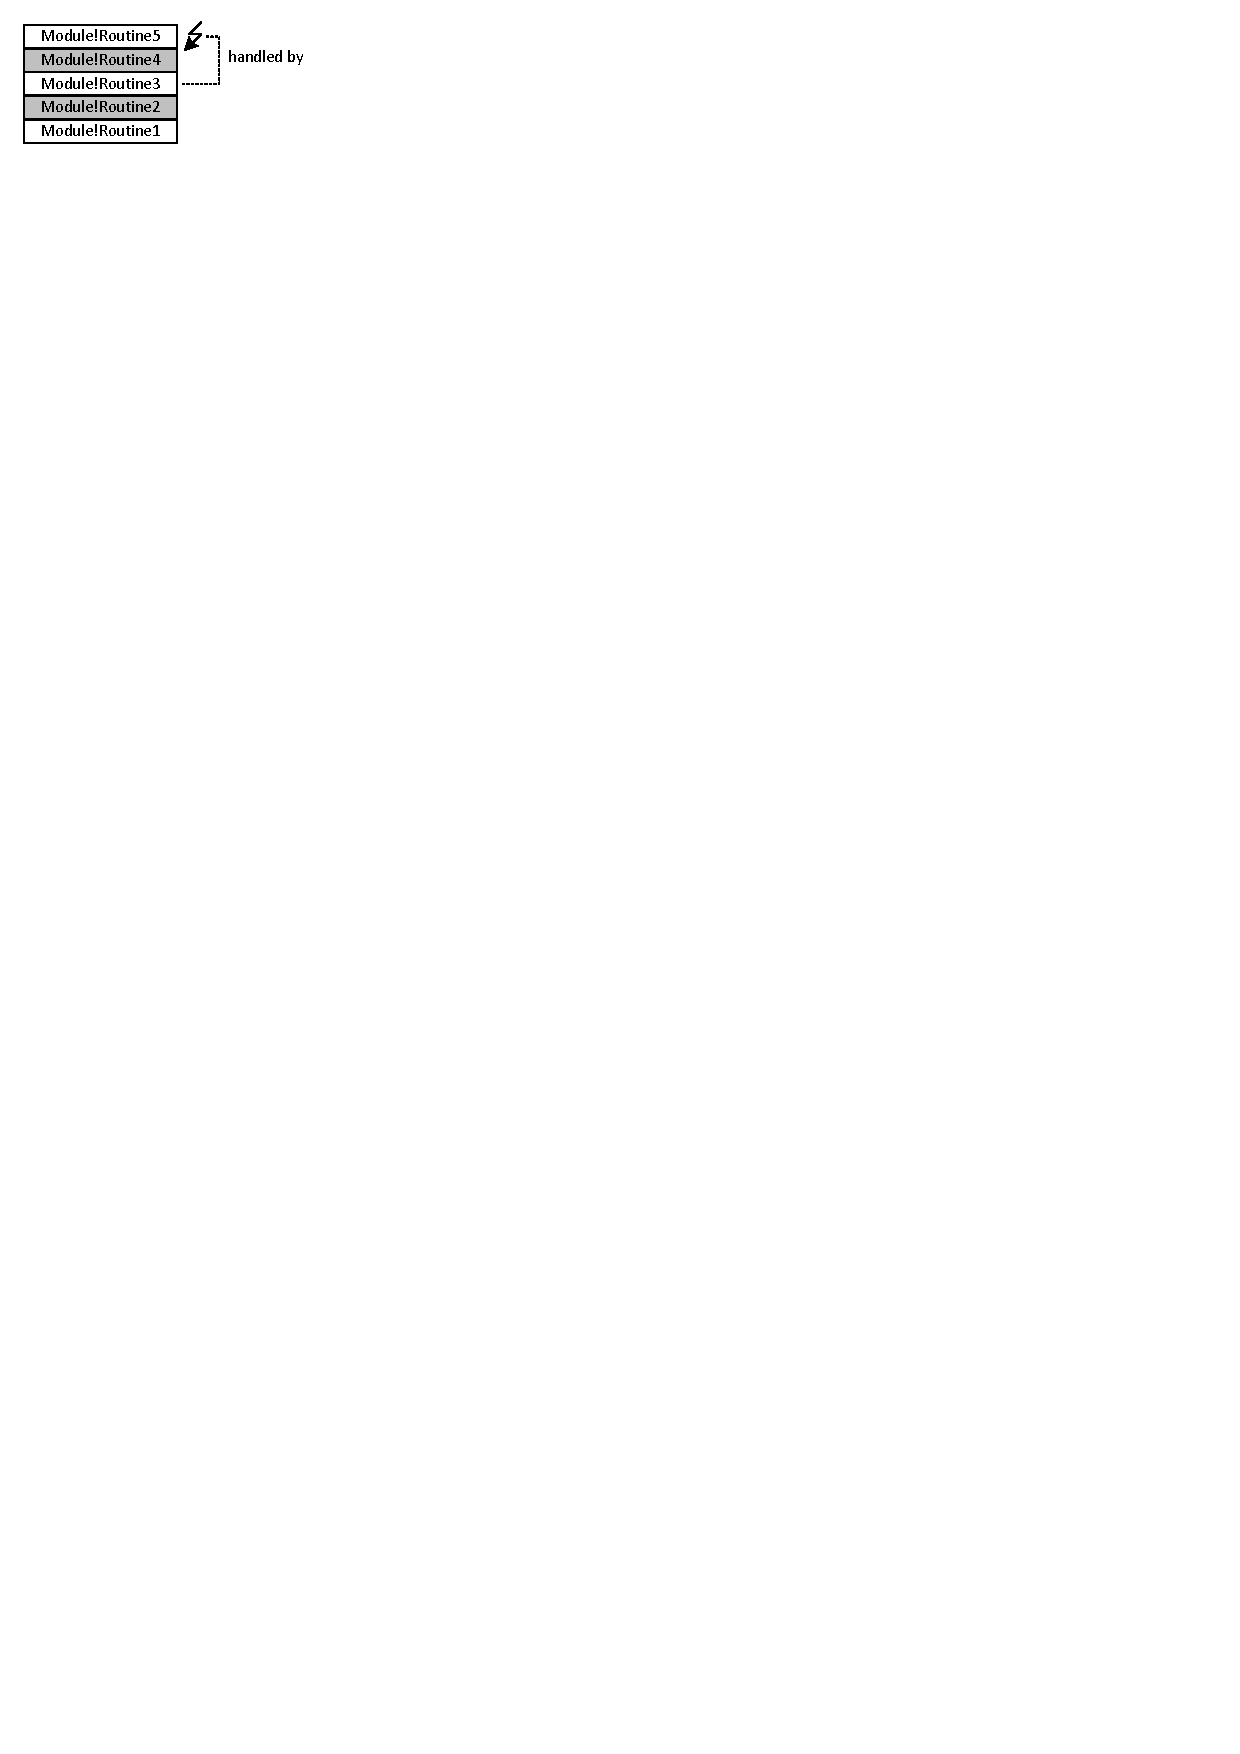
\includegraphics[scale=1.2, clip=true, viewport=0cm 27cm 5.5cm 30cm]{images/diagrams/Exception.pdf} 
\caption[An example callstack when an exception is raised]{An example callstack when an exception is raised. Gray boxes denote stack frames of traced routines.} 
\label{Exception} 
\end{centering} 
\end{figure}

The most critical issue, however, is what occurs in situations where there
are stack frames of traced routines on the callstack both, between the stack frame of routine raising and
the stack frame of routine handling the exception, as well as underneath the stack frame of the routine handling
the exception. An example for such a situation is illustrated by figure \ref{Exception}: 
Depicting a callstack, the stack is drawn growing bottom-up. Each box denotes a call frame,
gray boxes denote call frames of traced routines. \verb|Routine5| raises an
exception, which is handled by \verb|Routine3|. As discussed before, one
frame will now be leaked on the auxiliary stack. If \verb|Routine3| and
\verb|Routine2| later return, postprocessing for the latter routine has
to take place. That is, the topmost frame is popped from the auxiliary stack
and is used to obtain and reconstruct the original return address. However,
as the top frame denotes the leaked frame and is thus not the frame corresponding
to the call frame of \verb|Routine2|, this address will be wrong -- rather than
pointing into \verb|Routine1|, it will point into \verb|Routine3|. Needless to say,
continuing execution at the wrong return address will lead to behavior that may
be considered arbitrary.

Properly dealing with exceptions to avoid such interferences is thus of 
utmost importance. The implementation has to ensure that the auxiliary
stack is always kept in balance and in sync with the actual call stack.

\subsection{Structured Exception Handling}

SEH is available both in kernel and user mode. While user mode SEH is not
within the scope of this discussion, two things are worth pointing out: 
First, handling user mode exceptions requires the help of the kernel. That
is, user mode exception handling is not a pure user mode concept. Second,
both, user and kernel mode exception dispatching, are sufficiently similar to
be discussed jointly.

The workings of user mode SEH have been discussed in detail by \cite{Pietrek97}. 
Given their similarity, this discussion largely holds for kernel mode SEH as well. 

To allow a more detailed discussion of SEH and how it is relevant to 
function boundary tracing, the following section provides a brief overview 
of the inner workings of SEH. It is, however, crucial to notice that the
implementation of SEH on IA-32 differs fundamentally from the implementation
on AMD64. The remaining discussion is therefore largely IA-32-specific.

SEH is synchronous in that throwing and handling an exception only affects
a single thread. It is also built upon the notion of frame based exception 
handlers. That is, exceptions are not handled globally -- rather, each routine 
may associate an individual exception handler with its call frame. 

Short of hardware support on IA-32, SEH uses a programmatic approach to
maintain exception handlers and their association to call frames. Each
routine wishing to install an exception handler -- either to actually
handle an exception or at least to be notified about an exception, does 
so by creating an \verb|EXCEPTION_REGISTRATION_RECORD|. This structure
holds a function pointer to the exception handler routine that is to
be called during exception dispatching. To become effective, the structure
is registered by placing it in thread-locally maintained linked list
of registration records. These steps are usually done at the very beginning
of a routine. Accordingly, before the routine is left, the record must be 
unregistered by removing it from the linked list. The structure itself
\emph{must} be allocated on the stack.

The root of the list, i.e. the pointer to the topmost registration record
is located at the very beginning of the \emph{Thread Information Block} (TIB).
In user mode, the TIB is part of the TEB, in kernel mode, it is part of the
\emph{Processor Control Region} (PCR)\footnote{The PCR maintains processor-specific
state. The kernel maintains one instance of this structure per processor.}. 
In both cases, it is always accessible at offset 0 in the FS segment. Being part of the PCR 
rather than the KTHREAD, the dispatcher ensures that the pointer is updated 
whenever a different thread becomes subject to execution.

\subsection{Exception Dispatching Process}
When an exception is raised, the system walks the list of registration records,
calling each handler routine until it finds a handler agreeing to handle the
exception. This is implemented in \verb|RtlDispatchException|.
Focusing the discussion on the usual cases only,
a handler routine will return either \verb|ExceptionContinueSearch|, indicating
that the search for a handler shall continue, or \verb|ExceptionContinueExecution|,
indicating that the handler has handled the exception. Certainly, before a handler 
can return \verb|ExceptionContinueExecution|, a number of steps must have taken place.

There are basically two ways how an exception handler can deal with an exception. First, 
the handler can fix the reason for the fault and can request the faulting 
instruction to be retried by retaining the instruction pointer and returning
\verb|ExceptionContinueExecution|. Regarding traced routines, this situation can be 
deemed harmless.

The second, more common case is that execution is to be resumed elsewhere -- such as
in some exception compensation code located in the routine having installed the 
respective handler. However, continuing execution at a different address not
only requires the instruction pointer to be updated and returning 
\verb|ExceptionContinueExecution|, it also implies that the routines
corresponding to any outstanding call frames are about to be left prematurely. This is the 
situation where frames on the auxiliary stack are in risk of being leaked.

NT provides a dedicated routine for this purpose, \verb|RtlUnwind|. Before internally
calling \verb|ZwContinue| to perform the continuation, \verb|RtlUnwind| performs
a second phase of exception dispatching, \emph{unwinding}. During unwinding, each
routine about to be prematurely left is given the option to perform cleanup
work. That is, the list of exception registration records corresponding to the call 
frames in question is walked once more, and each handler is called again with a 
flag indicating that unwinding is taking place. Not before this phase has been 
completed is execution resumed at the new location.

Based on this brief summary of the exception dispatching process, it becomes clear
that whenever unwinding occurs, the auxiliary stack has to be unwound as well.

\subsection{Auxiliary Stack Unwinding}
\label{sec:Unwinding}
Adapting \verb|RtlUnwind| in the WRK to additionally trigger unwinding of the 
auxiliary stack seems possible, yet would have thwarted the intent 
of implementing the entire solution as a device driver and making it compatible
with the retail kernel. This approach has hence been dismissed.

To be notified about a call frame corresponding to a traced routine being unwound,
the natural approach is to leverage the SEH unwinding infrastructure itself. 
The basic idea is thus as follows: During preprocessing of a traced routine, an
additional exception handler is registered. Following general SEH practice, the
handler will be unregistered during postprocessing.

While this handler will merely return \verb|ExceptionContinueSearch| for all 
exceptions being dispatched, it will take additional action in case of an unwind: To
keep the auxiliary stack up to date, all it has to do is to pop its topmost
frame. 

Unfortunately, this approach is not viable in practice. Registering an additional
exception handler requires a \verb|EXCEPTION_REGISTRATION_RECORD| structure to be set up.
As noted before, SEH requires this structure to be allocated on the stack and
be accessible during the duration of the entire call. Yet, although the structure
occupies only 8 bytes, such stack allocation, as has been discussed
in section \ref{sec:ApproachOperation}, is infeasible to be made. 

Any attempts to store the registration record elsewhere, such as as part of the current 
frame in the auxiliary stack, are thwarted by the thorough validation logic
implemented both in \verb|RtlDispatchException| and \verb|RtlUnwind|.

Although the original idea kernel has been retained, the implementation therefore had to
be adapted in order to account for these special circumstances. Short of being able to 
allocate a dedicated registration record, the next underlying registration 
record is \emph{hijacked}: The existing pointer to the exception handler is 
exchanged against a pointer to the \emph{auxiliary stack unwinding exception handler}. 
This exchange is conducted during preprocessing of the traced routine. Accordingly, 
the modification is reverted during postprocessing. 

The handler itself, after completing its own work, will delegate the call to the original
handler having been replaced. That way, both handlers effectively share the same 
registration record. 

Certainly, this scheme requires the pointer to the original exception handler to 
be retained. Yet, the actual registration record does not offer space for storing an
additional pointer, so it has to be stored separately. Conceptually, the right kind 
of storage would be a thread-local map between pointers to registration records and 
pointers to the corresponding original handler routines.

In practice, however, a full-fledged map can be assumed to be not necessary. The
routine being looked up most frequently will always be the routine corresponding
to the topmost stack frame, followed by the routine of the second most recently
pushed stack frame, and so on. As a consequence, the implementation does not use
a separate map, but rather stores this information as part of the current stack 
frame of the auxiliary stack. 

To account for cases where the topmost frame does not contain the pointer being
looked for, the stack frame has been augmented by a pointer to the corresponding
exception registration record. That way, looking up the correct handler is a matter
of scanning the stack top-down, checking each pointer to the registration record,
and finally obtaining the corresponding pointer to the handler routine. As indicated
before, this scan can be expected to span few frames only, in most cases only the 
topmost frame.

Listing \ref{AuxStackFrame} shows the abbreviated structure defining an auxiliary stack frame.

\begin{lstlisting}[label={AuxStackFrame}, caption={Definition of an auxiliary stack frame}]
typedef struct _JPFBT_THUNK_STACK_FRAME
{
	//
	// Hooked procedure.
	//
	ULONG_PTR Procedure;

	//
	// Caller continuation address.
	//
	ULONG_PTR ReturnAddress;

	struct
	{
		//
		// Pointer to the (stack-located) registration record
		// corresponding to this stack frame.
		//
		PEXCEPTION_REGISTRATION_RECORD RegistrationRecord;

		//
		// Pointer to original handler that has been replaced.
		//
		PEXCEPTION_ROUTINE OriginalHandler;
	} Seh;
} JPFBT_THUNK_STACK_FRAME, *PJPFBT_THUNK_STACK_FRAME;
\end{lstlisting}

So far, we have implied that using a single exception registration record
for both the original and the auxiliary stack unwinding exception handler,
and performing proper call delegation yields the same functionality as 
using two separate registration records. However, this is not the case -- in fact,
there is a slight semantic difference that requires the scheme to be revised.

\subsubsection{Topmost Exception Handler Initiating an Unwind}

Figure \ref{ExceptionSimple} illustrates a situation in case no tracing is used.
One of the call frames (Routine3) has set up a SEH record. For the sake of
simplicity, this is the only record on the list of exception registration records
pointed to by the processor's PCR.

\begin{figure}[htbp] 
\begin{centering} 
%  (x, y), (x, y) from lower left corner
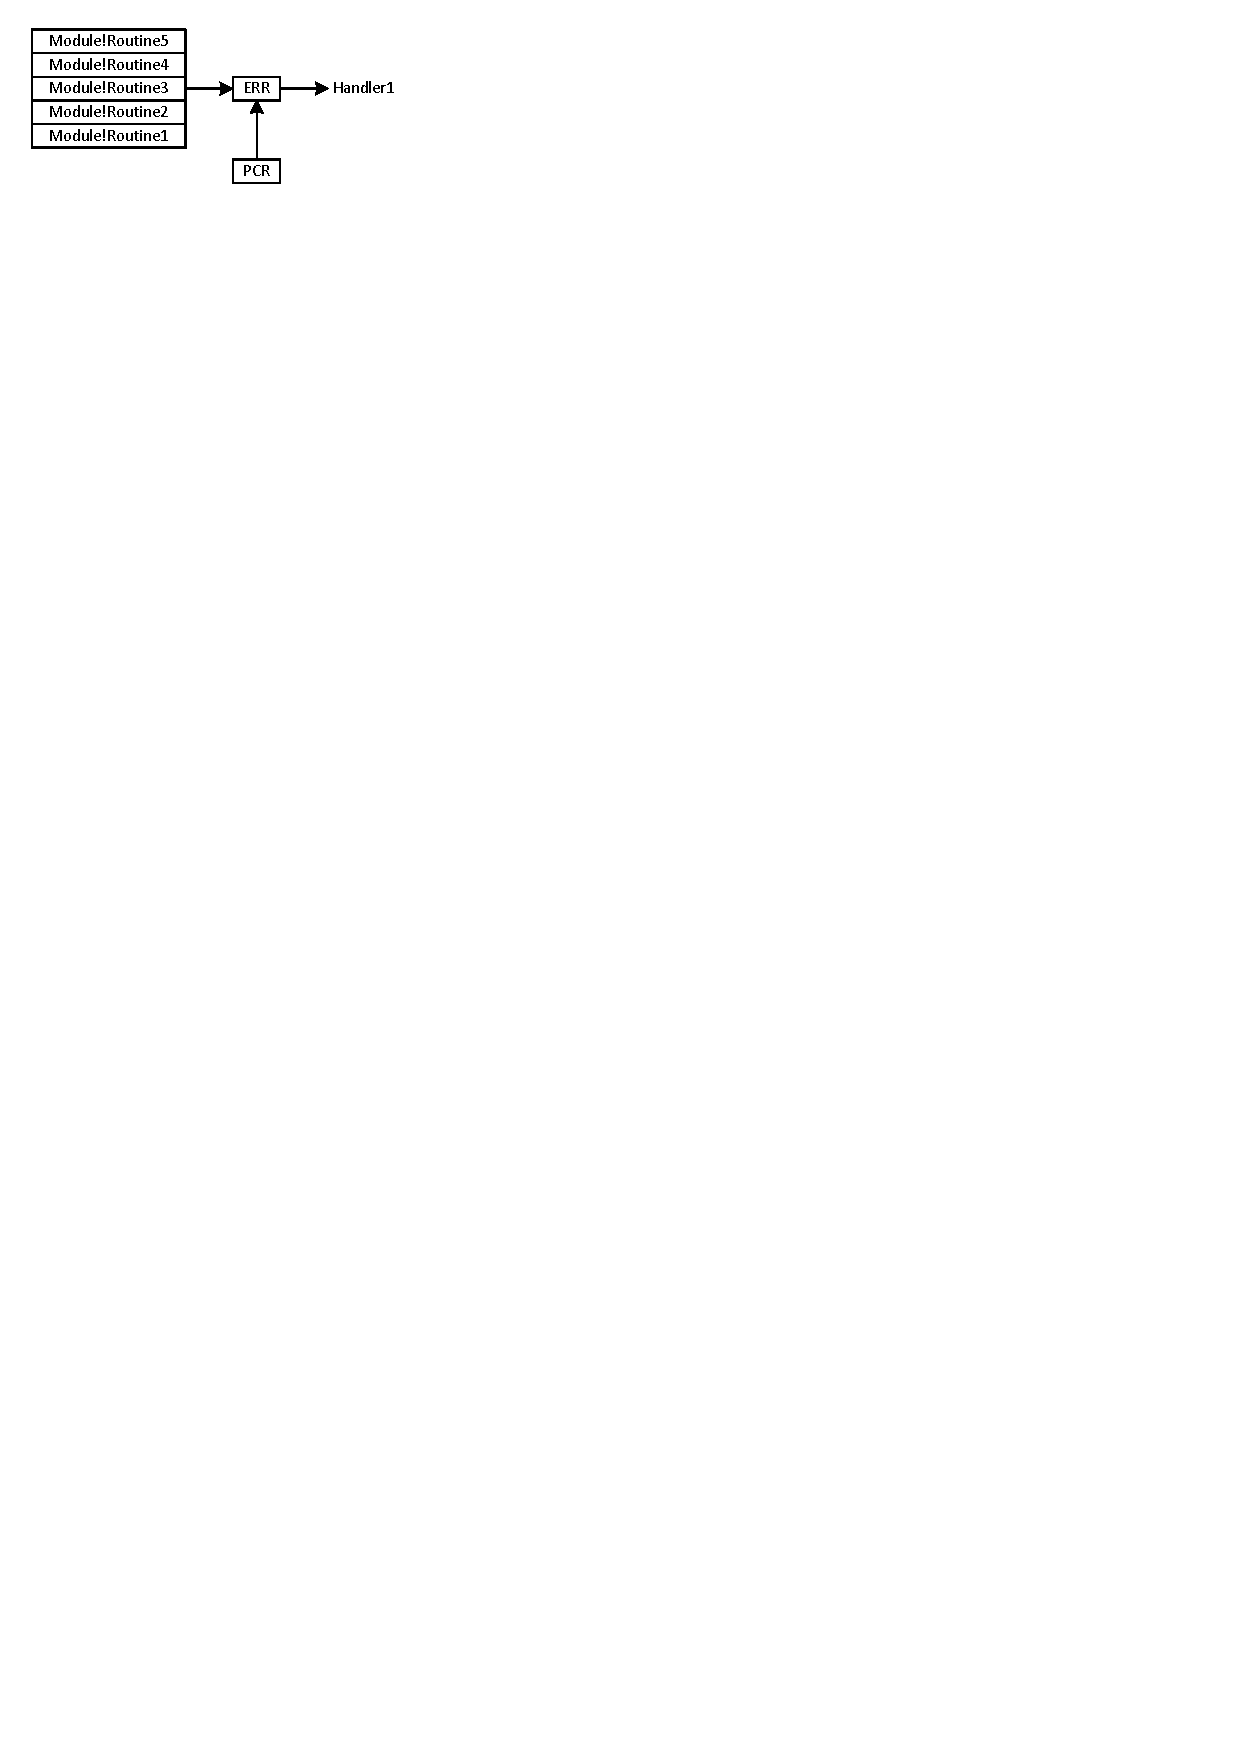
\includegraphics[scale=1.2, clip=true, viewport=0cm 26cm 8.5cm 30cm]{images/diagrams/ExceptionSimple.pdf} 
\caption[An example callstack]{An example callstack. ERR: Exception Registration Record.} 
\label{ExceptionSimple} 
\end{centering} 
\end{figure}

The same situation shall now be considered under the assumption that Routine4 has 
been instrumented for tracing. Following the technique discussed before, the
SEH record of Routine3 has been updated to point to the auxiliary stack 
unwinding exception handler. The pointer to the original exception handler has
been stored in the auxiliary stack frame corresponding to Routine4. The resulting
setup is illustrated in figure \ref{ExceptionSimpleWithInstr}.

\begin{figure}[htbp] 
\begin{centering} 
%  (x, y), (x, y) from lower left corner
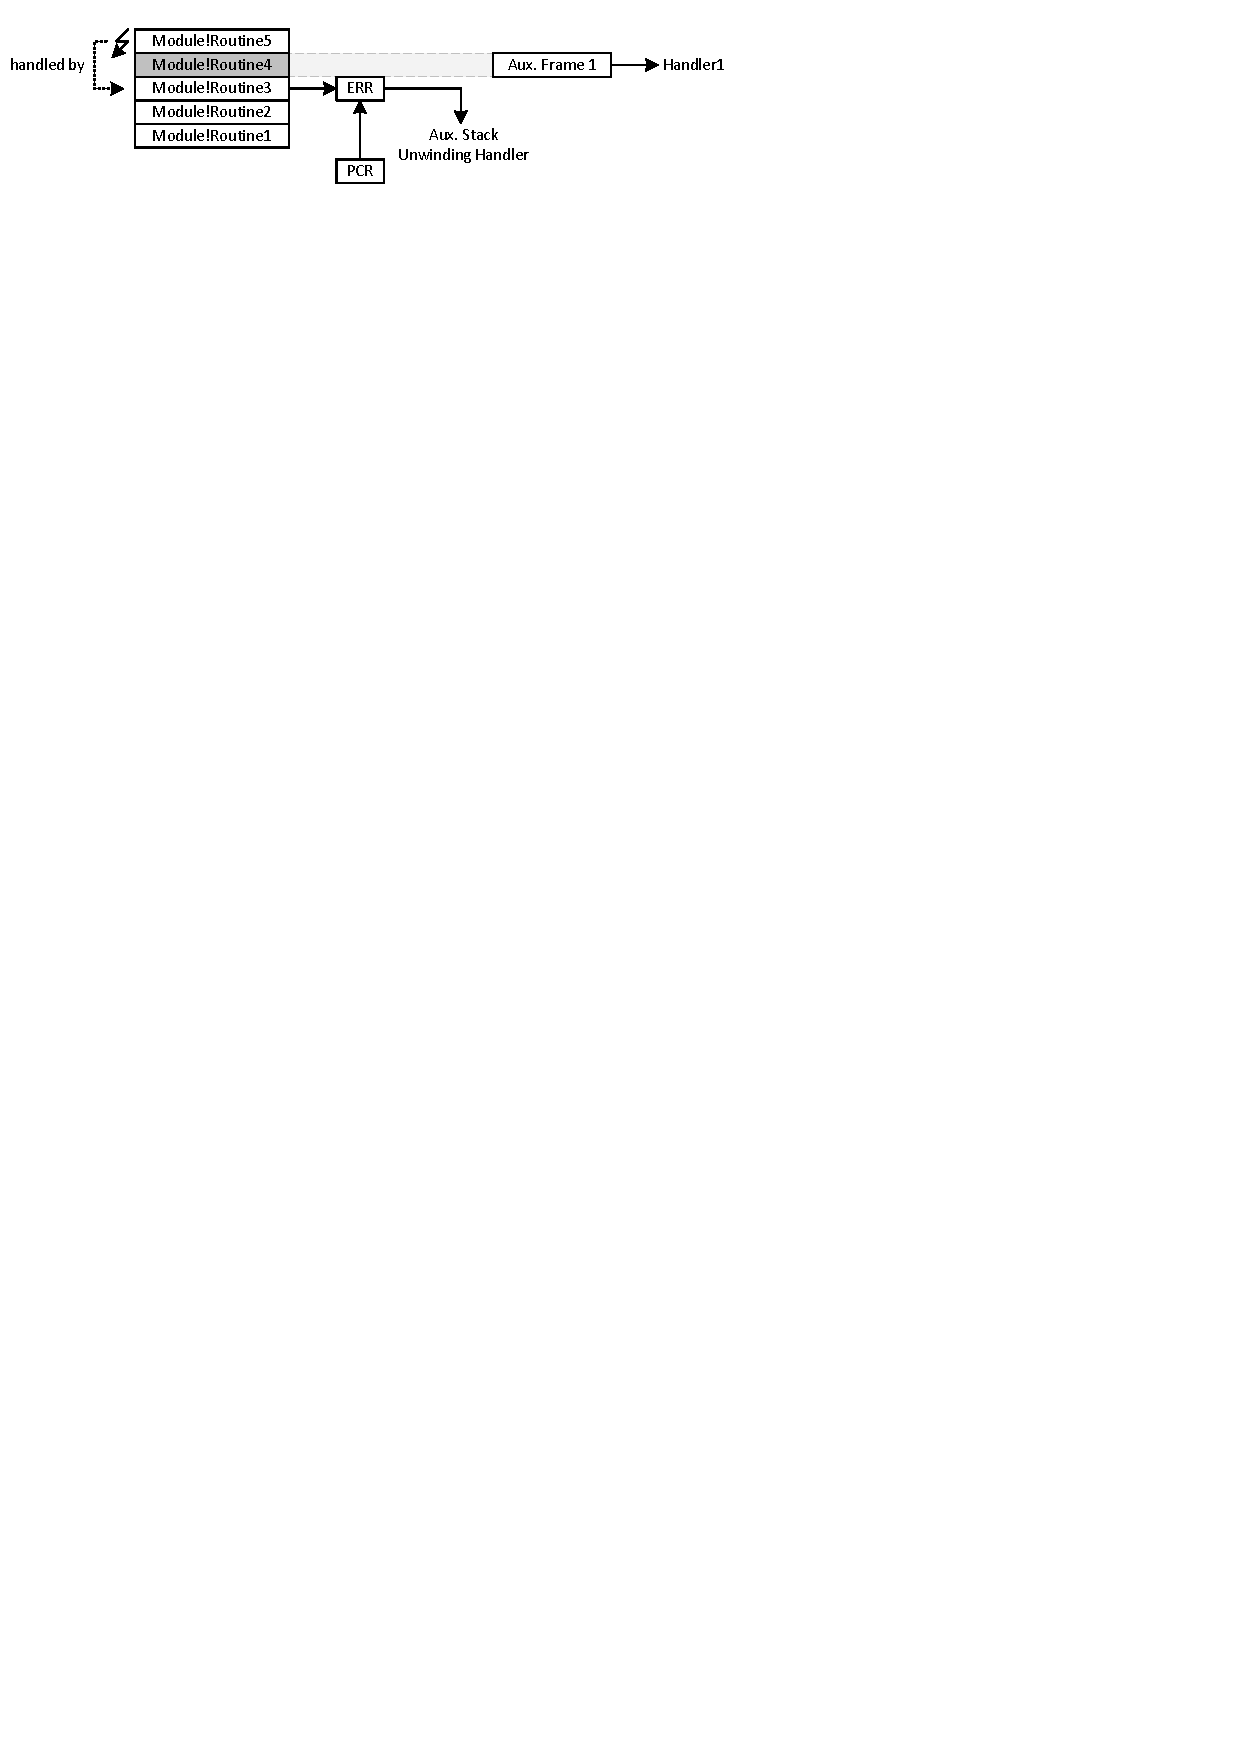
\includegraphics[scale=1.2, clip=true, viewport=0cm 26cm 17cm 30cm]{images/diagrams/ExceptionSimpleWithInstr.pdf} 
\caption[An example callstack containing a call frame of an instrumented Routine]{An example callstack containing a call frame of an instrumented Routine, Routine4.} 
\label{ExceptionSimpleWithInstr} 
\end{centering} 
\end{figure}

If Routine5 now raises its exception, \verb|RtlDispatchException| will first inspect
the SEH Record of Routine3 and invoke its handler, which is the auxiliary stack unwinding exception 
handler. Not yet knowing whether the exception will trigger an unwind or not, this routine will 
merely delegate the call to the original handler, Handler1, in order to let it make a decision.

We now assume that the original handler decides to handle the exception by continuing
execution in Routine3 and calls \verb|RtlUnwind| accordingly. 
However, \verb|RtlUnwind|, noticing that it has been the handler
of the topmost registration record that has handled the exception, 
realizes that no unwinding has to take place and will initiate
the continuation. While this behavior is clearly correct, the net result is
that the unwinding logic of the auxiliary stack unwinding exception handler has 
not been invoked. 

The underlying problem is that for the scheme to work, \verb|RtlUnwind| would
have to perform unwinding for all registrations down to \emph{and including}
the registration whose handler has handled the exception. Only in this case would
it invoke the unwinding logic of the auxiliary stack unwinding exception handler. However, as said,
\verb|RtlUnwind| rightfully excludes the latter from unwinding. 

Unaware of the fact that the registration record in question is actually
shared by two handlers, this leads to the situation where the auxiliary 
stack unwind fails to take place.

As such, the mechanism as discussed so far is not complete. There 
is, however, a way to mitigate this problem and cause \verb|RtlUnwind|
to always properly call the auxiliary stack unwinding exception handler. The
idea is as follows: The auxiliary stack unwinding handler is split
into two routines: The \emph{proxy exception handler} and the 
\emph{unwind handler}, both valid exception handler routines.

The unwind handler merely contains the auxiliary stack unwinding logic. That is,
when called, the routine unconditionally pops the topmost frame. Moreover, an appropriate
event callback routine is invoked. 

The proxy exception handler, as its name suggests, delegates to the original
exception handler. When called in the non-unwinding case, however, before the call is delegated to the 
original routine, an additional, full-fledged SEH frame is set up, specifying
the unwind handler as exception handler.

\begin{figure}[htbp] 
\begin{centering} 
%  (x, y), (x, y) from lower left corner
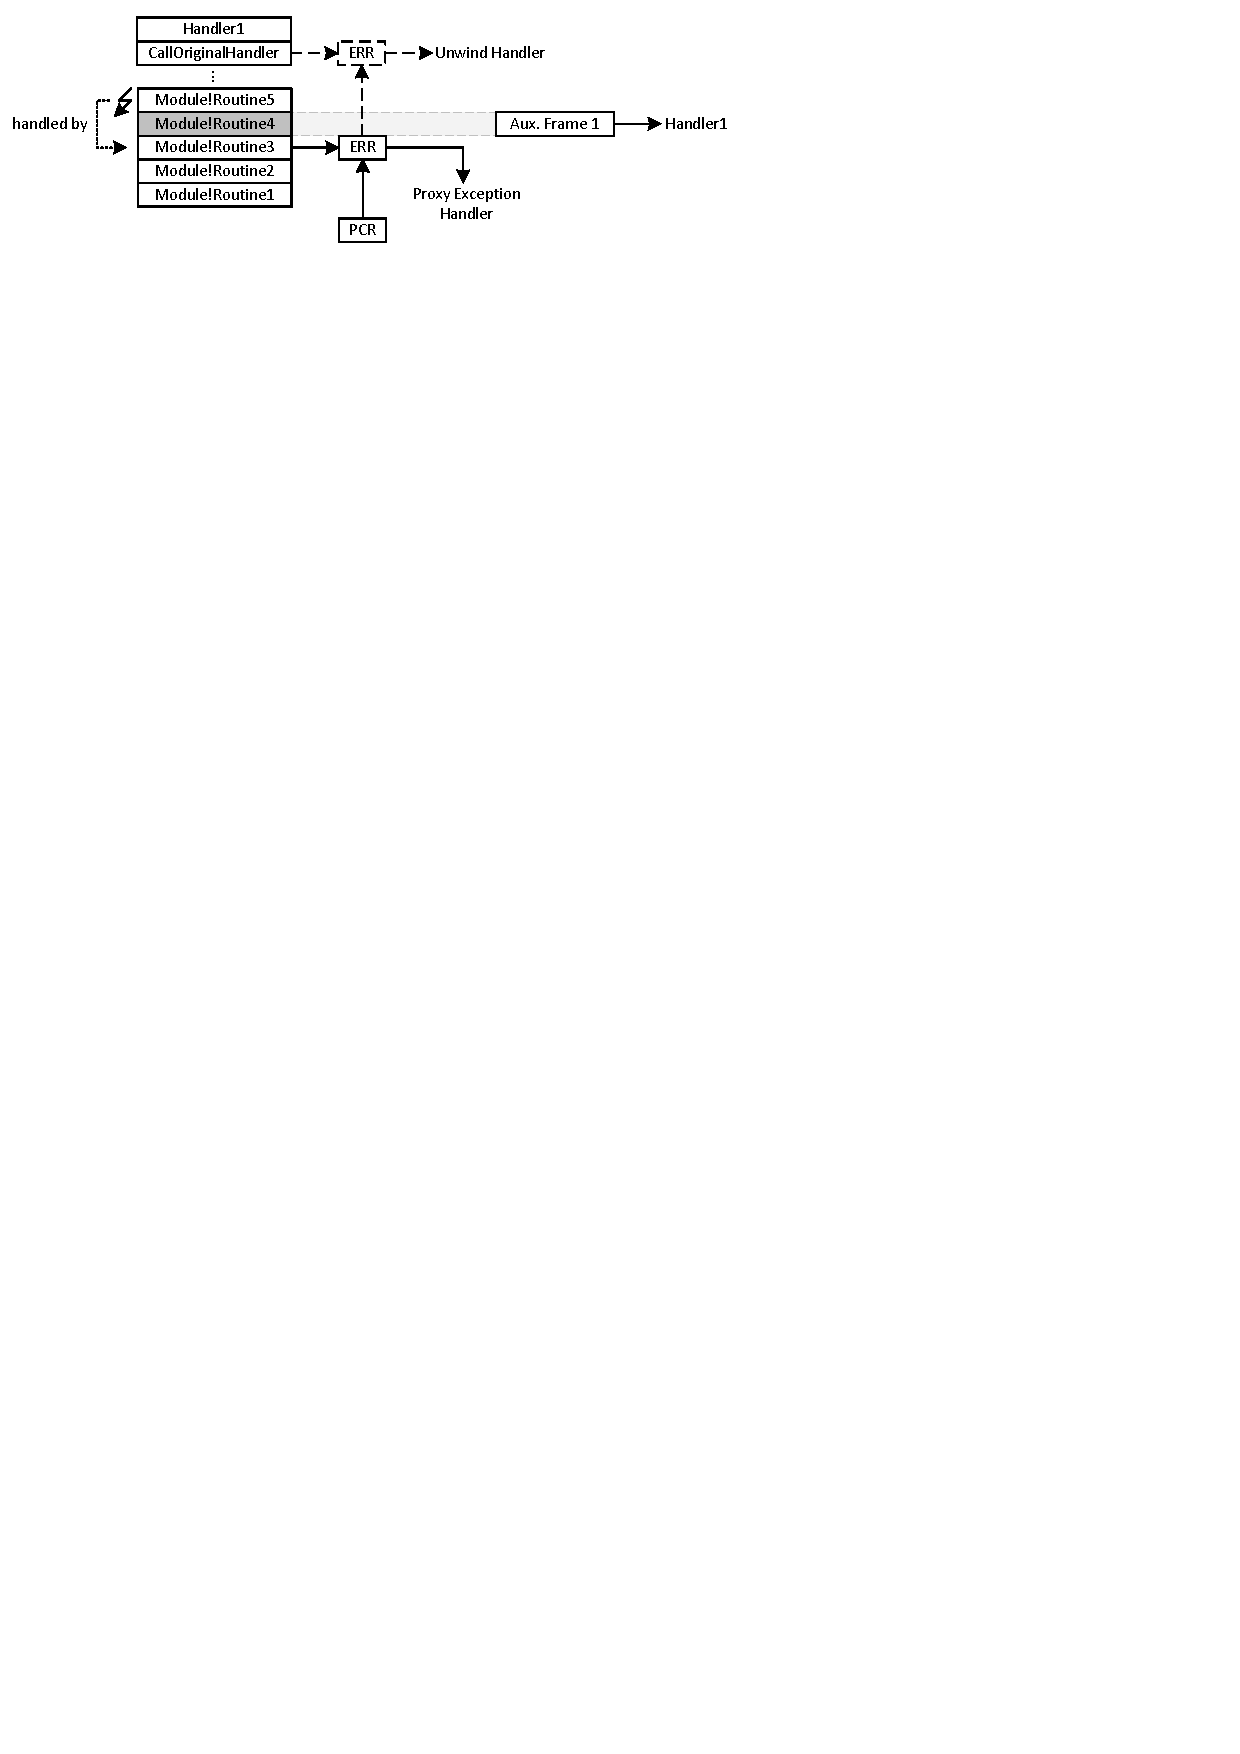
\includegraphics[scale=1.2, clip=true, viewport=0cm 25.5cm 17cm 30cm]{images/diagrams/ExceptionSimpleWithInstrNew.pdf} 
\caption{State during execution of the original exception handler} 
\label{ExceptionSimpleWithInstrNew} 
\end{centering} 
\end{figure}


Figure \ref{ExceptionSimpleWithInstrNew} illustrates the state at the point
where the proxy exception handler has delegated the call to the original
handler: The SEH chain now temporarily contains an additional registration record,
illustrated with dashed lines.

Revisiting the situation discussed before, the behavior of \verb|RtlUnwind|
will now change. Although the SEH record installed by Routine3 has been the
top record when the exception occurred, it is not the top record any more when
the exception is dispatched. Noticing this, \verb|RtlUnwind| will now unwind
the top record, which involves calling the unwind handler: The auxiliary stack
can now be properly unwound.

\subsubsection{Non-Topmost Exception Handler Initiating an Unwind}
The situation slightly changes when more than one exception registration is 
involved and not the topmost, but rather a handler of one of the bottom registration
records agrees to handle the exception. This situation is illustrated in
figure \ref{ExceptionSimpleWithInstrBottom}: Routine2 and Routine4 have been
instrumented; Routine 5 raises an exception, Routine2 will finally handle the exception. The handler of the
topmost exception registration record (corresponding to Routine4), which is the proxy exception handler, is 
invoked first. Like in the previous example, it will set up a temporary registration 
record (not shown) and will delegate the call to Handler2. However, Handler2 declines to handle 
the exception and returns \verb|ExceptionContinueSearch|.

\begin{figure}[htbp] 
\begin{centering} 
%  (x, y), (x, y) from lower left corner
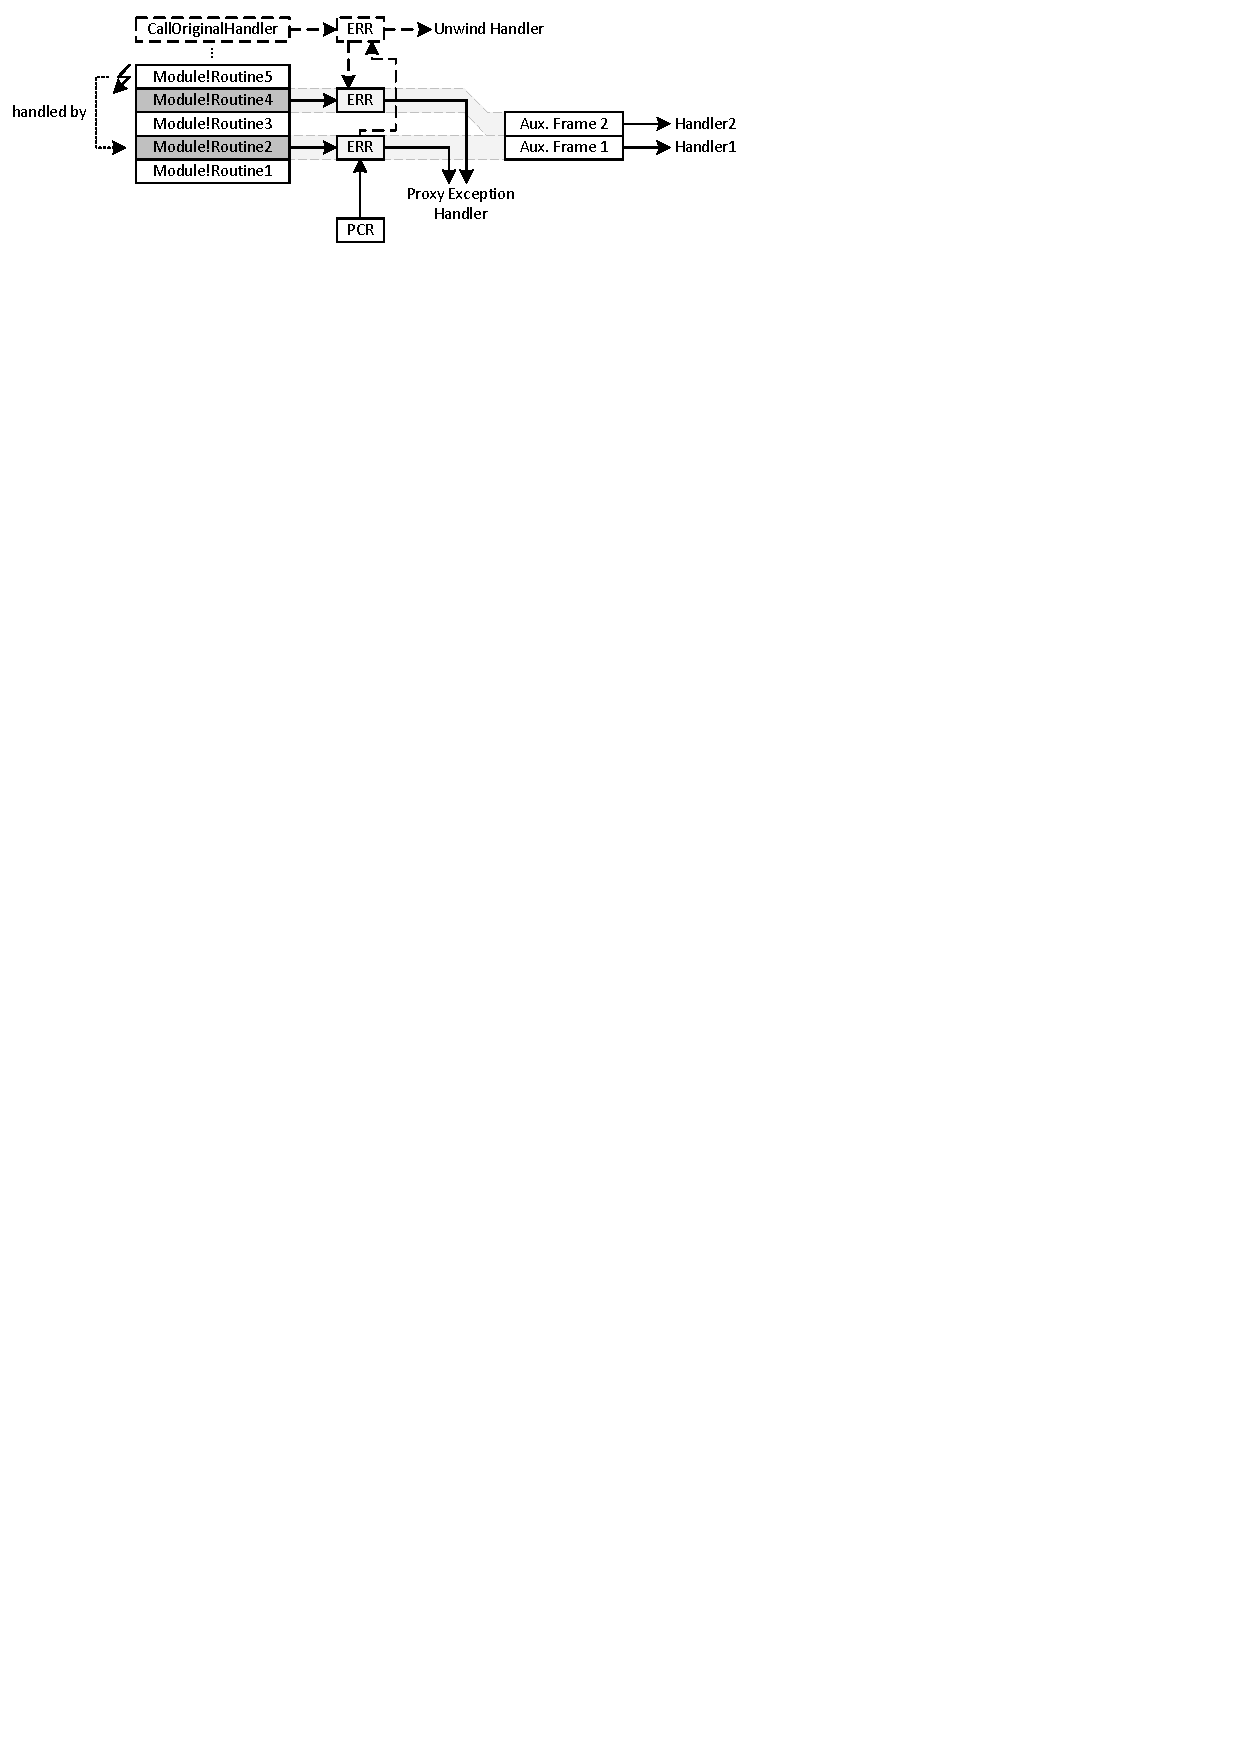
\includegraphics[scale=1.2, clip=true, viewport=0cm 25.5cm 17cm 30cm]{images/diagrams/ExceptionSimpleWithInstrBottom.pdf} 
\caption{Bottom handler handling the exception} 
\label{ExceptionSimpleWithInstrBottom} 
\end{centering} 
\end{figure}

Proceeding with the next exception registration record, the proxy exception handler
is called again. This time, however, a different auxiliary stack frame applies and
the call will be delegated to Handler1. Again, a temporary registration record is set 
up before invoking the handler (shown with dashed lines). Handler1 agrees to handle 
the exception and initiates an unwind by calling \verb|RtlUnwind|.

As indicated before, \verb|RtlUnwind| will walk the list of registration
records once more. That is, it will first invoke the handler associated with
the topmost registration record, which, again, is the proxy exception handler.

Unlike the previous call, however, the handler is requested to perform unwinding.
In this case, it will pop off the topmost auxiliary stack frame, and will
delegate the call to Handler2.

The next registration in the chain is the temporary registration installed before
Handler2 was invoked. Its handler, the unwind handler, is invoked and will pop
off the last outstanding auxiliary stack frame, which is Frame 1. At this point, unwinding
has been completed and the auxiliary stack has properly been unwound.

\subsubsection{Multiple Instrumented Routines Sharing a SEH Record}
So far, only situations have been considered where the number of stack frames
of instrumented routines, and thus the number of auxiliary stack frames, matched 
the number of SEH registration records on the stack. When more than one 
auxiliary stack frame maps onto a single SEH registration record, a slight variation
of the scheme is required, as figure \ref{ExceptionSimpleWithInstrMulti} suggests.


\begin{figure}[htbp] 
\begin{centering} 
%  (x, y), (x, y) from lower left corner
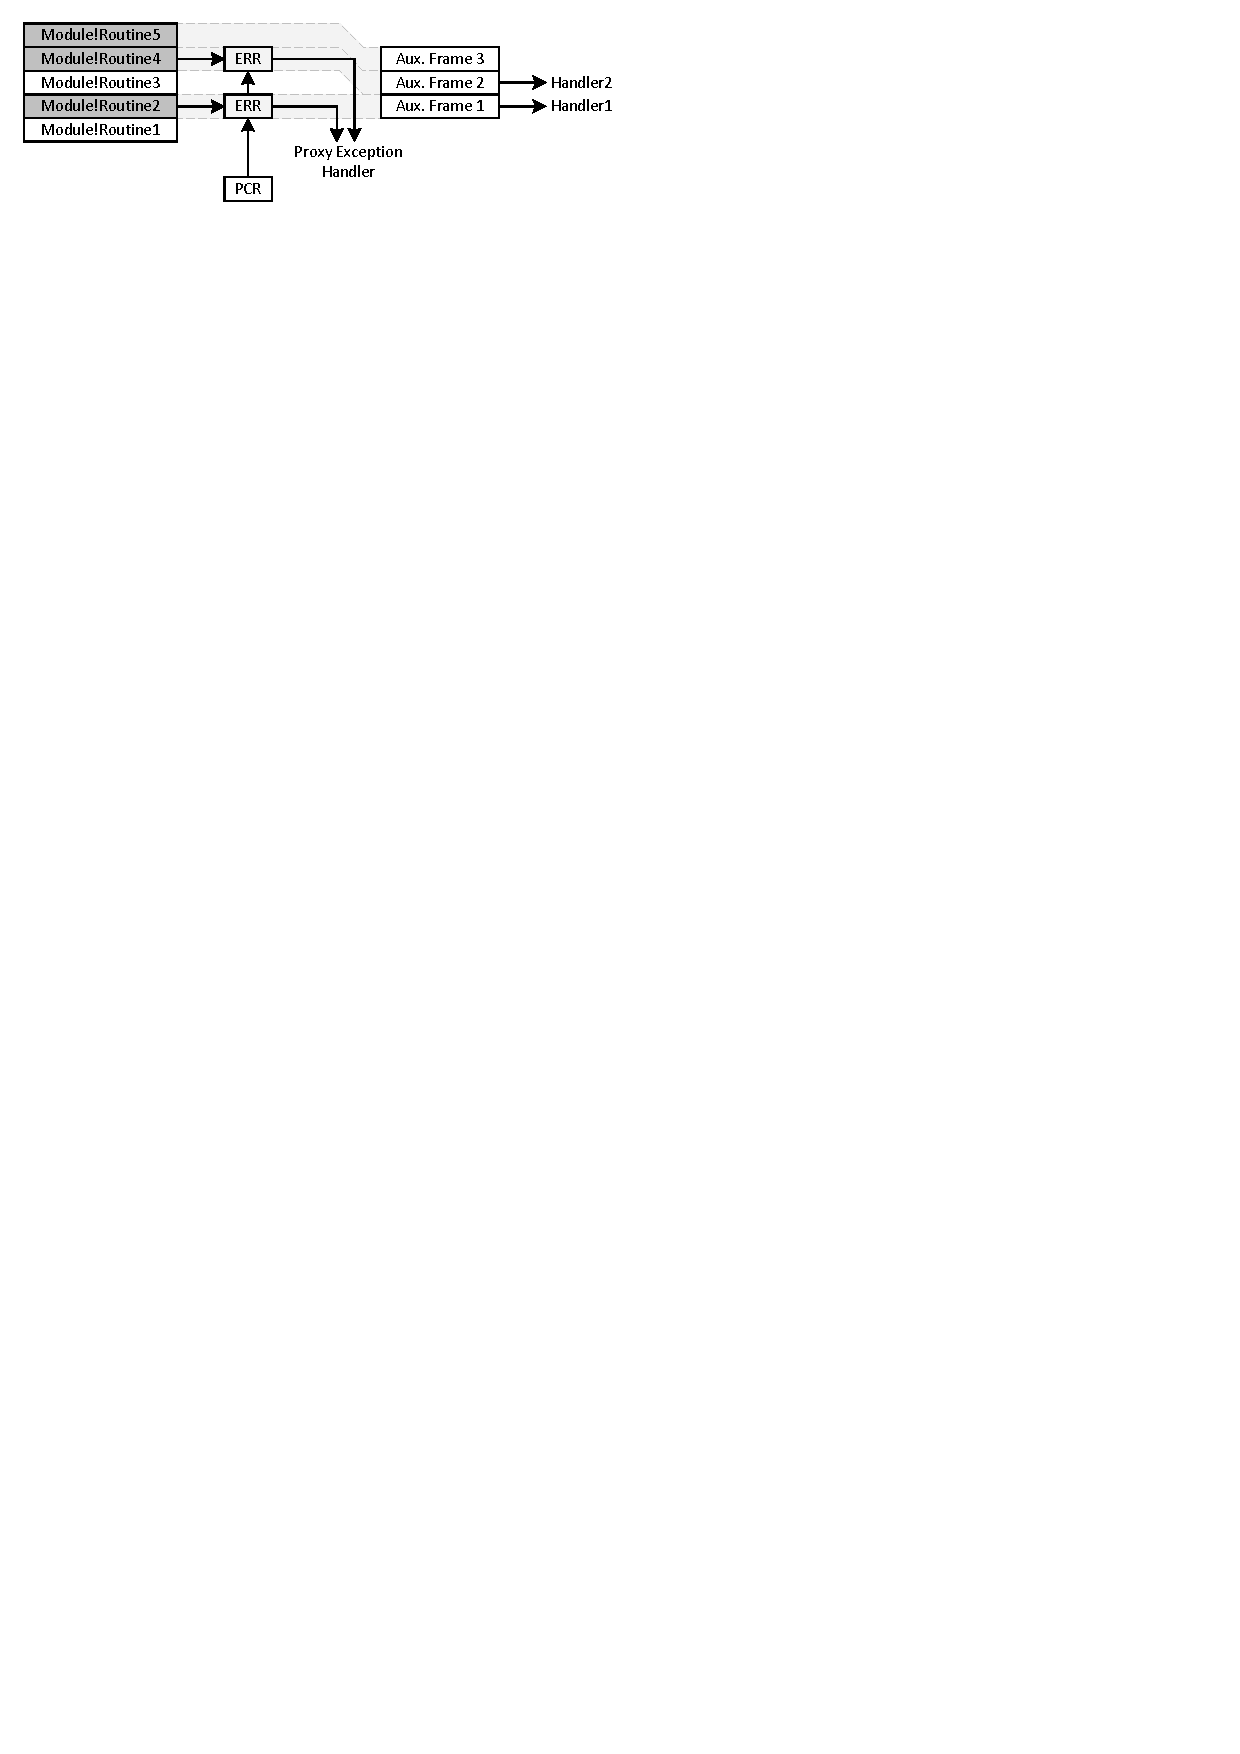
\includegraphics[scale=1.2, clip=true, viewport=0cm 26cm 11cm  30cm]{images/diagrams/ExceptionSimpleWithInstrMulti.pdf} 
\caption[Multiple auxiliary stack frames mapping onto a single registration record]{Multiple auxiliary stack frames mapping onto a single exception registration record} 
\label{ExceptionSimpleWithInstrMulti} 
\end{centering} 
\end{figure}

If the respective registration record is found to already point to the proxy exception handler (as 
in the case of Routine5), the handler
is not replaced once again. Rather, the auxiliary stack unwinding logic accounts for such
situations: Instead of popping only the topmost frame, a call to the unwind handler or 
the unwind part of the proxy exception handler causes all frames up to and including the first frame 
containing a pointer to an original exception handler routine to be popped. In the specific
case depicted by figure \ref{ExceptionSimpleWithInstrMulti}, this means that the
auxiliary stack frames 2 and 3 would be unwound at once, while frame 1 is unwound
in isolation.



\subsubsection{Empty SEH Chain}
Another situation that has been ignored so far is the possibility that no
SEH record has yet been installed when a traced routine is called. That is,
the respective pointer in the PCR contains the special value \verb|EXCEPTION_CHAIN_END|.

In such situations, the scheme as discussed so far is not applicable. It is,
however, also not necessary to install an additional exception handler in 
this case: If no SEH record has been installed and one of the functions
indirectly called by the traced routine raises an exception while still no
SEH frame has been set up, this exception will necessarily be left unhanded 
and lead to a bugcheck. The fact that an auxiliary stack frame 
has been leaked is in this case of no real concern as the system is about to
stop anyway. 

As a consequence, if the PCR is found to not have a single exception
registration record registered, the entire process of installing an additional
exception handler can safely be skipped.

Finally, it is worth mentioning that the entire implementation is SafeSEH-conforming.


\section{Event Handling}
\label{sec:EventManagement}
Besides the ability to capture events such as procedure entry and exit, a 
vital component of a tracing solution is the handling of such events. Being in charge
of recording, buffering and persisting potentially large volumes of event 
information, event handling also plays a critical role for the performance 
of a tracing solution. 

Although exact numbers depend on the number of routines instrumented, tracing
on the level of routines must be assumed to generate significant amounts of data. 
Especially when tracing is enabled for longer periods of time, storing event information
in memory must therefore be assumed to be too expensive in terms of resource consumption. 
Persisting the information to secondary storage is clearly favorable.

Writing event information synchronously to disk from within the event callback routines
invoked on entry or exit of an instrumented routines can be assumed to be both 
prohibitive for performance and reentrance reasons. An asynchronous approach -- 
temporarily storing the information in memory and having a background thread periodically 
write the data back to disk -- promises to be advantageous in both counts.

One implementation approach could thus be to collect event information in kernel 
mode memory and having a user mode program collect the information data via appropriate
system calls or shared memory. Once retrieved, the program would write the data 
to a trace file.

Utilizing the Windows NT kernel mode I/O API, however, it is possible for a kernel
mode component to directly access and write files, i.e. without having the data be 
relayed by a user mode program. Requiring less system calls and less memory to 
be copied, this approach can clearly be expected to be more efficient and has thus
been chosen for NTrace.

\subsection{Buffer Management}

A variety of buffer management strategies exist for such asynchronous tracing 
approaches. Not aiming to be exhaustive, a list of three basic approaches shall
be briefly discussed:
\begin{itemize}
	\item	Maintaining buffer space shared among all processors and threads. 
	\item Processor-private buffer space -- each processor is assigned buffer space
		that may only be used by code running on this processor.
	\item Thread-local buffer space -- each thread is associated private buffer space.
\end{itemize}
Regarding synchronization, reentrance, ordering and anticipated cache 
behavior, each of these approaches has its individual advantages and shortcomings.

\subsubsection{Synchronization}
Synchronizing access to buffer space among concurrently executing threads is 
required for the approach utilizing a globally shared buffer. For 
processor-local and thread-local buffer space, concurrent access cannot occur
and synchronization is not required.

\subsubsection{Reentrance}
Although concurrent access cannot occur for the latter two approaches, they are,
like the first approach, prone to reentrance-related issues. Regardless of
the individual implementation, allocating and writing an entry to buffer space
can be assumed to be non-atomic, i.e. requiring multiple CPU instructions.

This non-atomicity can become a problem as soon as interruptions occur. Unless 
the IRQL prevents it, interrupts, and, indirectly, \emph{Deferred Procedure Calls} (DPC)
as well as \emph{Normal} and \emph{Special Kernel Asynchronous Procedure Calls} (APC) can
interrupt code at any time. Running on the same processor/thread, these routines 
could either themselves be instrumented or may call instrumented routines.
In either case, when the interrupted routine has been in the midst of writing an 
entry to buffer space when it was interrupted, reentrance will occur as soon
as the interrupting routine attempts to write its first record to buffer space.

In order to protect against corruption of such thread- or processor local resources,
it is thus vital for the respective code to properly deal with reentrance.

\subsubsection{Ordering}
In order to be of worth, event information as stored in buffer space and trace 
file must obey a defined order. Only if ordering of events can be assumed, it is
possible to derive further information such as caller/callee-relations.

Whether total ordering of events across all processors and threads is required
or not depends on the individual application. If events such as context switches
or lock acquisitions are traced, which have a global impact, total ordering of
events may be indispensable.

Routine calls are inherently thread-local, although for certain applications,
seeing which routines were executed concurrently may depict valuable information.
For the majority of use cases, however, it may be expected that threads will be
inspected in isolation and partial ordering, in which only events originating 
from the same thread are ordered w.r.t. each other, is in fact sufficient.

If total ordering is required, using globally shared buffer space is the natural
choice. By the use of other means such as sequence numbers, it is, however,
also possible to maintain total order if separate buffer spaces are used, as
in the case of CPU- or thread local buffers. Yet, the latter two schemes may be
expected to achieve their maximum efficiency when only partial ordering is required.

\subsubsection{Cache Behavior}
If instrumented routines are called at a high frequency, the memory occupied by
buffer space can become a \emph{hot} resource. While this is not problematic
per se, it can lead to inefficiencies on multiprocessor machines when the buffer space
is shared among processors. If events are produced on several processors at 
roughly the same rate, certain cache lines will repeatedly be updated from 
different processors in an alternating fashion. This, however, can lead to bus
contention and pipeline stalls, which in turn will induce a non-negligible 
performance overhead \cite{Win2000Perf}. Thread- or processor-local caches
can be expected to exhibit more beneficial cache behavior in this regard.

\subsubsection{Implementation Choice}
\label{sec:BufferImplementation}
Concluding the brief discussion of buffering approaches, it is clear that each
approach has its individual strengths and weaknesses and neither is capable of
suiting all needs. As such, the choice of a buffering approach has not been 
hardwired in the core library. Rather, the user of this library, which, in 
the architecture laid out, is the \emph{Kernel Function Boundary Tracing Agent},
decides on the buffering scheme to implement.

The WRK/WMK version is capable of leveraging the WMK infrastructure for event
buffering, which internally uses globally shared buffer space \cite{Schmidt08}. Not only will
total ordering of events be preserved in this case, the function boundary
tracing events will also be ordered with respect to the other events captured
by the WMK such as context switches.

The version of the agent targeting the retail Windows kernel uses a custom
buffering scheme, following the approach of using thread-local buffer space 
providing partial ordering. When the agent is loaded, a certain amount 
of equally-sized buffers is allocated from the non paged pool and are kept 
in a global list, the \emph{free list}. 
Typical buffer sizes range between 64 and 256 KB.

\begin{figure}[htbp] 
\begin{centering} 
%  (x, y), (x, y) from lower left corner
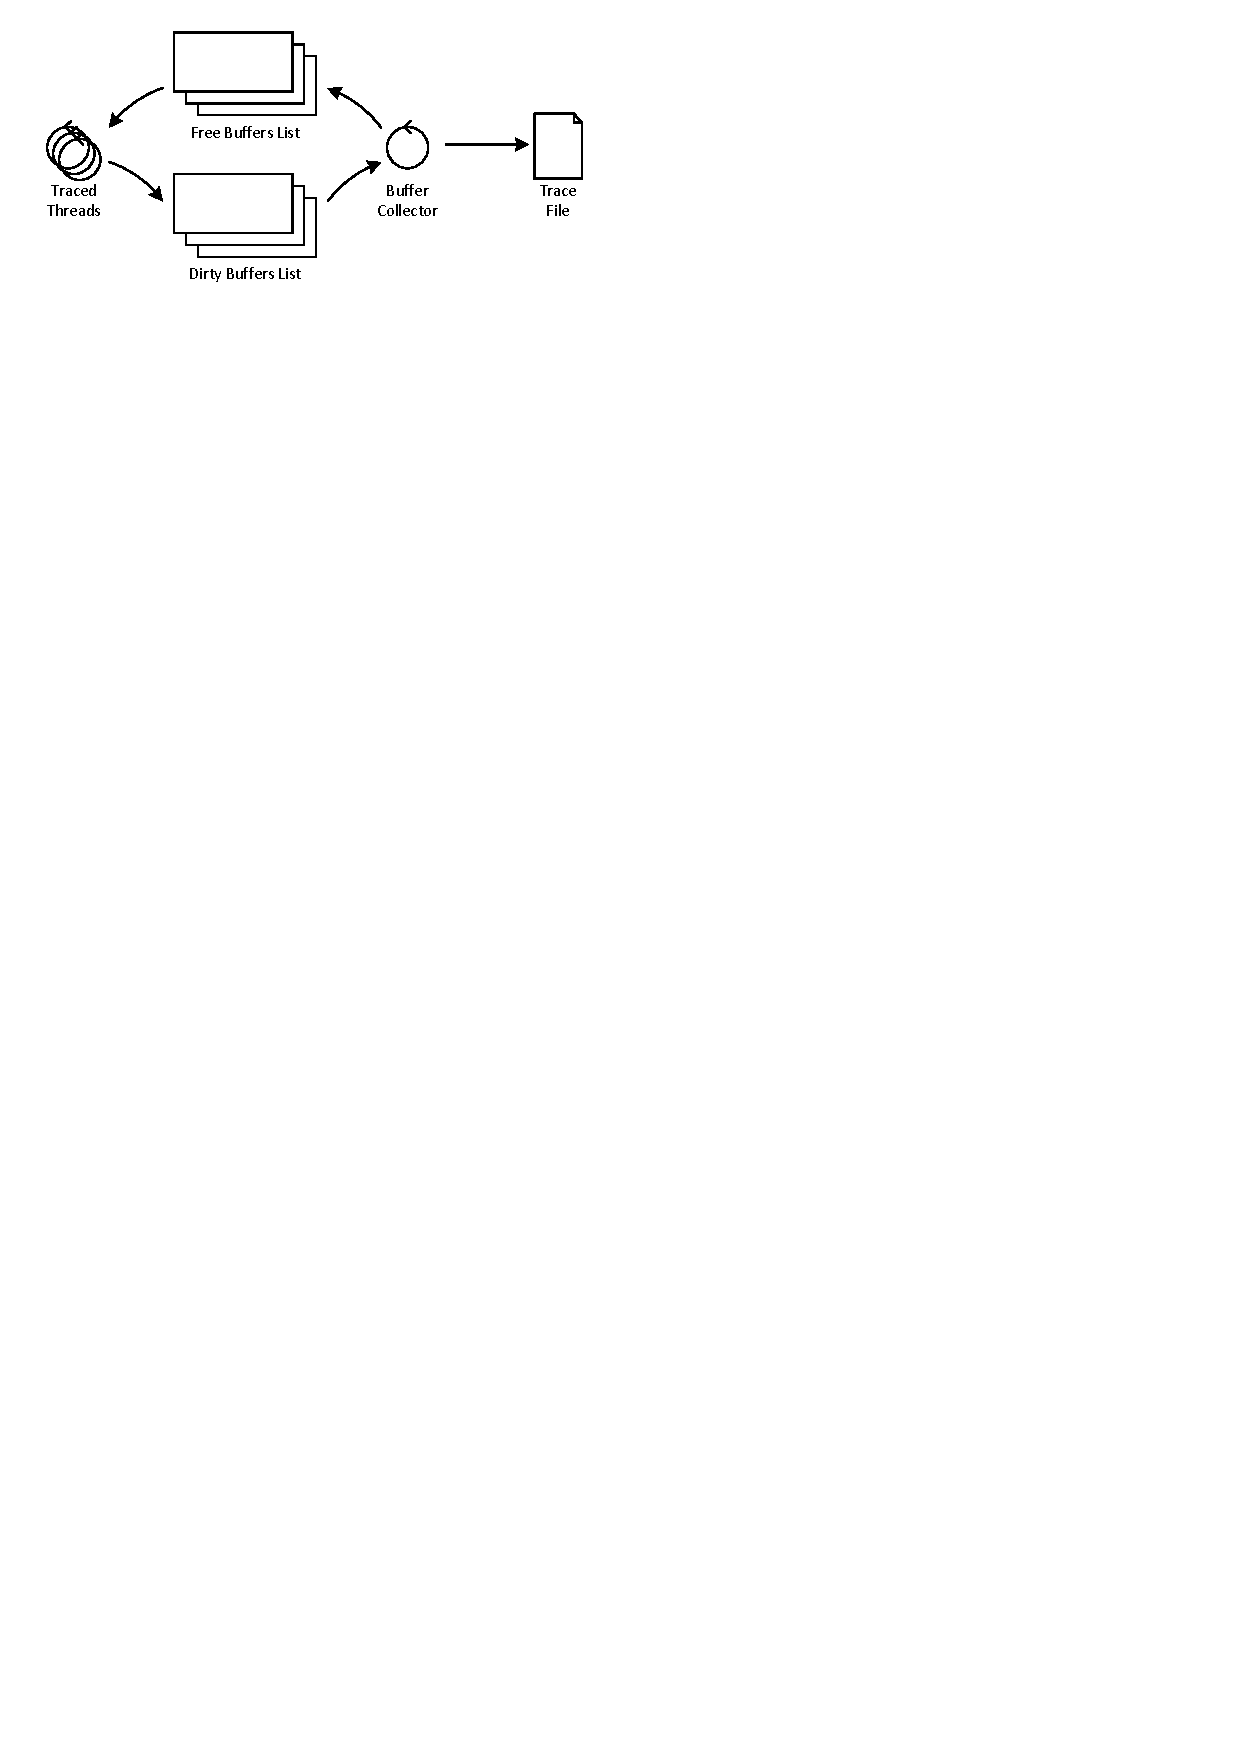
\includegraphics[scale=1, clip=true, viewport=0cm 24.5cm 10.5cm 30cm]{images/diagrams/BufferDynamics.pdf} 
\caption{Buffer Management Dynamics} 
\label{BufferDynamics} 
\end{centering} 
\end{figure}

Figure \ref{BufferDynamics} illustrates the key idea of the implementation. As soon as an event is
to be written to buffer space, a buffer has to be obtained from the free list.
Using atomic operations, a buffer is removed from this list and attached to the
current thread, where it will be used until its space is exhausted. If the next event
is to be stored, the existing buffer is put on another global list, the \emph{dirty list}
and a new, empty buffer is obtained from the free list.

Periodically, the \emph{buffer collector}, a dedicated system thread, will take 
each buffer from the dirty list and flush its content to the trace file. 
After reinitializing the buffer, it is re-added to the free list.

A number of aspects of this approach are worth highlighting. Exclusively relying
on interlocked \emph{SList} functions, the entire buffer management implementation can be
characterized as being lock-free. Regarding cache behavior, the implementation limits
interaction with global memory to obtaining and releasing buffers. As one buffer
is capable of holding several thousand events, this interaction occurs on a less 
frequent basis. Finally, using thread-local buffers allows storing certain information
such as thread and process identifiers once per buffer, rather than once per event
record, which in turn helps cutting the size of event data.

Finally, protection against reentrance issues is provided by the mechanism
implemented by the CallProxy and EntryThunk. This mechanism has been discussed
in section \ref{sec:ThunkReentrance}.

\subsection{Timing}
In order to allow making judgments about timing behavior, trace events 
may include a timestamp reflecting the time at which the routine 
entry or exit event was captured. Based on these timestamps, the time
elapsed during the invocation of a routine can be easily calculated.

To be effective, the timer used for taking these timestamps should satisfy 
at least the following requirements:
\begin{itemize}
	\item Taking a timestamp should not induce a significant performance impact.
	\item Time should advance monotonically and at a constant rate.
	\item As many routines can be expected to complete in significantly less 
				than 1 millisecond, the timer resolution should be below 1 millisecond.
	\item Time as observed by different processors should be synchronous. Alternatively, the 
				clock skew should be bounded to a value small enough to not have a 
				significant impact on the correctness and value of time measurements.
\end{itemize}

Not aiming to be exhaustive, the following list shows the prevalent sources for 
timing information offered by the Windows NT kernel API:

\begin{itemize}
	\item System Time, available via \verb|KeQuerySystemTime|.
	\item Tick Count, available via \verb|KeQueryTickCount|.
	\item Interrupt Time, available via \verb|KeQueryInterruptTime|.
	\item High Resolution Performance Counter, available via \verb|KeQueryPerformanceCounter|.
	\item Bypassing the API, \verb|rdtsc| can be used to obtain the \emph{Time Stamp Counter} (TSC).
\end{itemize}

The first three sources all provide a resolution in the order of 10 milliseconds and
are thus unsuitable for obtaining the desired timestamps. \verb|KeQueryPerformanceCounter|
supports fine-grained resolution, yet, the exact behavior of this routine 
depends on a number of factors. \verb|KeQueryPerformanceCounter| is part of 
the \emph{Hardware Abstraction Layer} (HAL) and its implementation differs
between the uniprocessor and multiprocessor HAL. Moreover, it may use different 
time sources depending on hardware configuration. Short of public documentation
on this topic, variations among operating system releases should also be expected.

Potential time sources used by \verb|KeQueryPerformanceCounter| include
the \emph{ACPI timer} (also referred to as PM clock), \verb|rdtsc|, and the
\emph{8254 Programmable Interval Timer}\footnote{Note that this information has been obtained from disassembly as no
authorative information on this topic seems to be available to date.}. 
As of Windows Vista, the \emph{High Precision Event Timer} (HPET) is also supported.

Although \verb|KeQueryPerformanceCounter| provides a clean abstraction of
the inhomogeneity among hardware, this variance makes it hard to judge
the applicability of the function for the specific usage scenario. Assuming the
8254 timer is not being used, \verb|KeQueryPerformanceCounter| can be expected to
execute quickly and provide sufficient precision. However, especially when the TSC is
used (either via \verb|KeQueryPerformanceCounter| or directly by using \verb|rdtsc|),
it is crucial to notice that synchronicity is not guaranteed. 

The TSC is maintained on a per-processor basis and is guaranteed to advance 
monotonically \cite{intel07_2B}. It is, however, crucial to notice that due to
power management, significant skew between the TSC values of different 
processors of a multiprocessor system may emerge \cite{Brunner05}.

If a thread is migrated from one processor to another while in the midst of
performing time measurements, this clock skew can easily render the timing measurements 
performed by this thread meaningless. Worse yet, it is possible that the TSC of 
the second processor is behind the TSC of the first processor, so that time has 
effectively went backwards for the thread having migrated. 

Unless such processor migrations are explicitly prohibited by using thread-affinity,
neither synchronicity nor monotonicity may thus be assumed for the TSC on 
a multiprocessor machine.

A detailed discussion of the advantages and disadvantages of the various timers 
and strategies to deal with clock skew is beyond the scope of this work. 
Despite its lack of guarantees on multiprocessor machines, both 
\verb|KeQueryPerformanceCounter| and \verb|rdtsc| have been used in practice
for providing the timestamps. While achieving good results on
uniprocessor machines, the implication on multiprocessor machines is that
timing results become flawed as soon as TSC skew emerges.

%The \emph{8254 Programmable Interval Timer}, which seems to be used as a last
%resort, provides only coarse-grained resolution of about 1 millisecond. Moreover,
%its use requires disabling interrupts, which induces significant overhead. Both the
%ACPI timer and the TSC provide suffiently fine-grained resolution.
%
% only. Moreover, obtaining the time requires reading from an I/O 
%port and induces a significant performance overhead. The \emph{APIC timer} as
%well as the \emph{High Precision Event Timer} (HPET), are also not yet available 
%on all hardware.
%
%This leaves the \emph{ACPI timer} (also referred to as PM clock), and the
%\emph{Time Stamp Counter} (TSC) for use as a time source. 
%
%Both the \emph{8254 Programmable Interval Timer} (PIT) and the 
%\emph{Real-Time Clock} (RTC) support timer resolutions of 1 millisecond only.
%Moreover, obtaining the time requires reading from an I/O port and induces a
%significant performance overhead.
%
%Although a detailed discussion of this topic is beyond the
%scope of this work, the following discussion provides a brief summary.


\subsection{Symbols}
The most vital part of an event record is the information which routine has 
just been entered or left and is thus the cause of the event. Hence, each
event record contains the \emph{virtual address} (VA) of its corresponding routine. 

Alternative options to handle this information would have been to use the 
\emph{relative virtual address} (RVA), i.e. the offset of the routine
relative to the containing module's load address or the name 
string of the routine. The latter option would necessitate a certain 
amount of symbol handling or maintenance of a mapping between addresses 
and names to be managed in kernel space, which was undesired. Moreover,
storing names requires significantly more buffer space, which is a scarce 
resource. 

Calculating the RVA requires a non-negligible amount of processing as well --
which is unfortunate for three reasons: Firstly, it slows down a code path that
must be expected to be executed at high frequency. Secondly, this processing
may have to occur at elevated IRQL -- calling certain APIs to perform the calculation may thus not be feasible. Finally,
the additional processing would increase the danger of reentrance, as the API
routines called during the conversion process may themselves be instrumented.

The burden of converting from VA to RVA and finally to 
a name is thus put on the application reading the trace file. For this to 
work, the trace file contains two critical pieces of information for each
module for which routines have been instrumented: The load address, which
is required for conversion between VA and RVA, and the debug information
of the module, which is part of the module's PE image and is required for
identifying the symbol files exactly matching the module. Given this information,
it is possible to read a trace file and properly resolve all symbol information --
even in the case where the operating system release and file versions differ between
the machine having produced and the machine reading the trace file.

\subsection{Call Nesting}
\label{sec:CallNesting}

The event records stored in the trace file should allow reconstructing the call flow
and the nesting of calls on each thread. For this to work, pairs of entry and exit
event records must be found that both correspond to a single routine execution. 
As event records are written sequentially, finding these pairs should be possible
solely based on their order in the trace file (respecting the fact that entries may
origin from different threads). Figure \ref{NestingOk} illustrates this idea by 
showing a trace of a very simple program: A function \emph{Main} calls \emph{Foo},
which in turn calls \emph{Bar}.

\begin{figure}[htbp] 
\begin{centering} 
%  (x, y), (x, y) from lower left corner
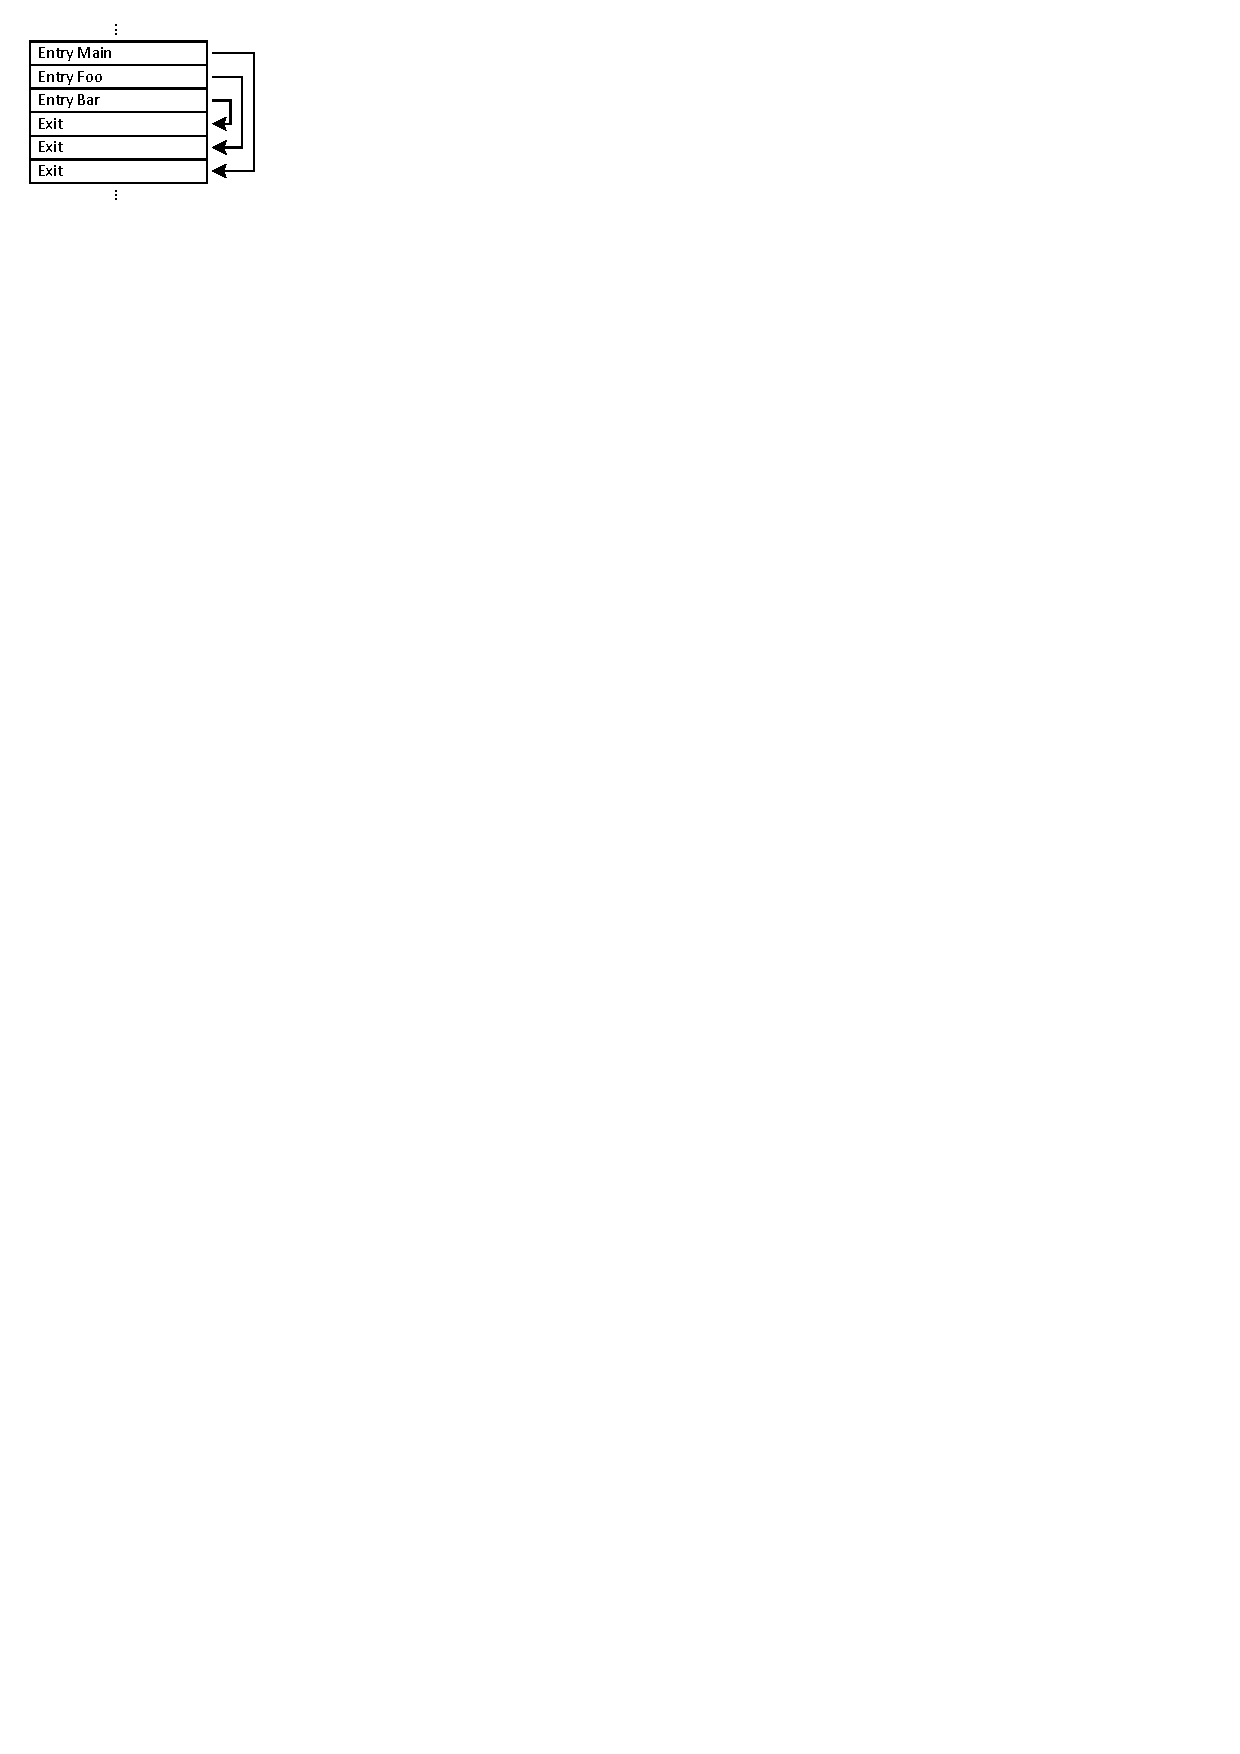
\includegraphics[scale=1, clip=true, viewport=0cm 26cm 5cm 30cm]{images/diagrams/NestingOk.pdf} 
\caption{Finding pairs of event records} 
\label{NestingOk} 
\end{centering} 
\end{figure}

This approach, however, fails as soon as events have to be dropped due to resource
constraints. When buffer space for storing event records is depleted and no
empty buffer space can be obtained, events have to be dropped. Picking up the previous
example and assuming that the exit event record for \emph{Bar} could not be written
due to memory shortage, the resulting trace looks as illustrated in figure 
\ref{NestingWithMissingRecords}.

\begin{figure}[htbp] 
\begin{centering} 
%  (x, y), (x, y) from lower left corner
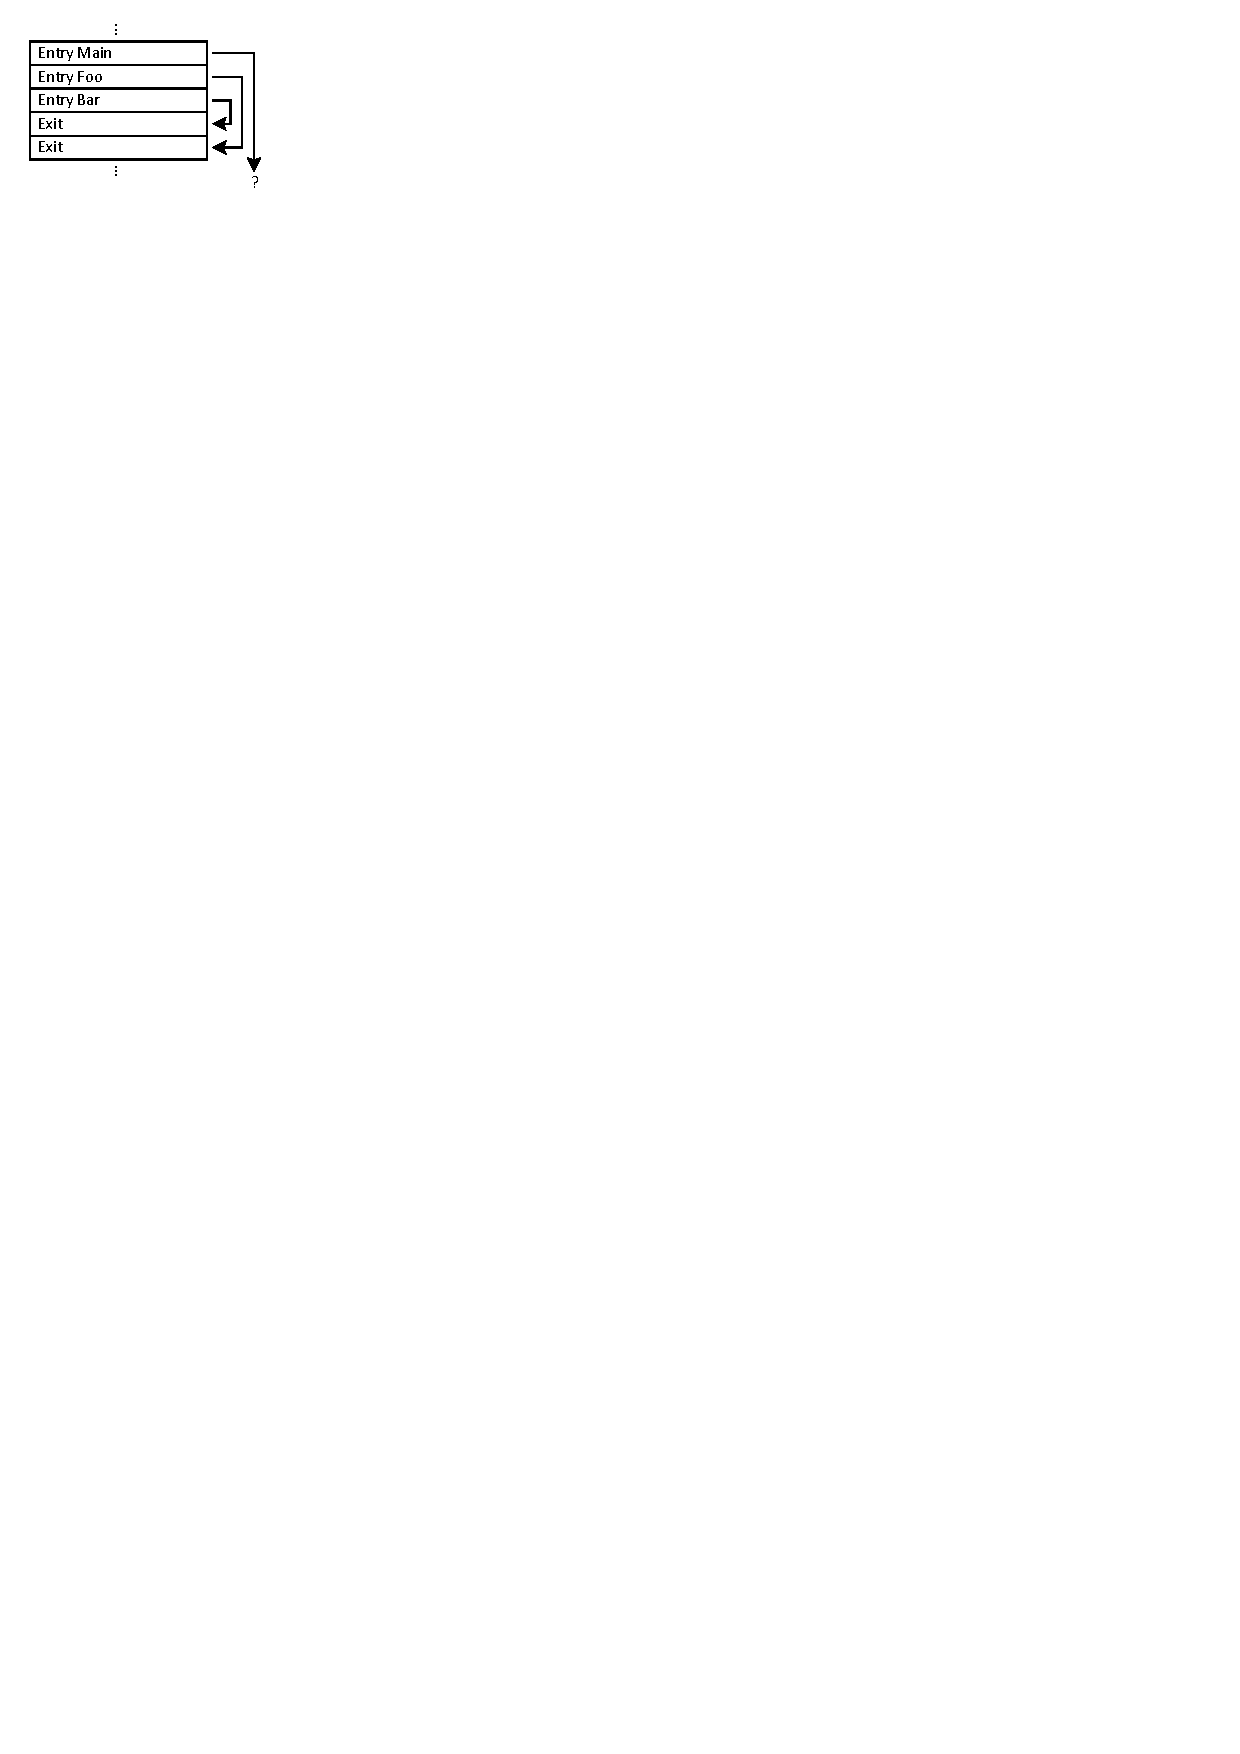
\includegraphics[scale=1, clip=true, viewport=0cm 26.5cm 5cm 30cm]{images/diagrams/NestingWithMissingRecords.pdf} 
\caption{Finding pairs of event records in case of lost events} 
\label{NestingWithMissingRecords} 
\end{centering} 
\end{figure}

The fact that the count of entry and exit event records does not match any more
indicates exit event losses. Yet, based on this data, it is not possible to decide 
on which exit event has in fact been lost. Not being able to properly match entry-
and exit events any more thwarts any attempts to correctly reconstruct nesting 
relationship among calls.

To avoid such situations from occurring, the implementation approach differs in that
all exit events include the routine address. As this address is not available any 
more during call postprocessing, it is preserved as part of the auxiliary stack frame.

Having the routine address included in exit event records now allows sanity checks
to be made when reading the file. If a pair of entry and exit events does not have
matching addresses, it is safe to assume that at least one entry or exit event must
have been lost between these two records. To a certain extent, this even allows
implying which events must have been lost. Being able to simulate such events 
significantly improves the quality of resulting trace analysis. 

\section{Concluding Remarks on Runtime Code Modification}
Employing runtime code modification, it is crucial for NTrace to properly address
the challenges of runtime code modification that have been discussed in 
chapter \ref{sec:ChallengesOfRuntimeCodeModification}. Although the mechanics used to
overcome these challenges have already been considered in the previous sections,
they are worth being summarized.

Due to the focus on the IA-32 architecture and Windows NT using the flat memory model, 
no special considerations regarding the memory model are necessary. Concerning memory
protection, however, NTrace has to deal with wrtite-protected portions of images. As 
discussed in section \ref{sec:ApplyingThePatches}, additional virtual address mappings 
are used to circumvent such protection mechanisms. 

NTrace also generates code during runtime -- namely, the jump necessary to divert execution
from the original routine to the trampoline as well as the trampoline itself. Yet, this 
code is used to override existing code, i.e. it is written to memory which can be assumed to 
grant \emph{execute} permissions already. As such, no special measures have to be taken in 
order to comply with the restrictions of Data Execution Prevention.

As discussed in section \ref{sec:ApproachOperation}, the jump used to divert execution to the trampoline
uses a fixed jump distance. The distance of the jump from the trampoline to the CallThunk, however,
varies depending on the location of the routine being instrumented and the load address of the
FBT agent driver. However, as both origin and target of the jump fall into kernel virtual address space,
the distance is guaranteed to be smaller than 2 GB in size. As 2 GB also is the maximum distance
supported by the near jump instruction used, jump-distance related issues are avoided.

Regarding cross-modifying code and atomicity, NTrace follows the guidelines defined by 
Intel \cite{intel07_3A}. The implementation of the respective algorithm, which is based on
the usage of DPCs, has been discussed in section \ref{sec:ApplyingThePatches}.
Yet, usage of this algorithm alone does not protect against the issues of concurrent 
execution (section \ref{sec:ConcurrentExecution}) as well as preemption and interruption 
(section \ref{sec:PreemptionAndInterruption}). 

During instrumentation, these issues are
avoided by the fact that NTrace only replaces a single instruction (the \verb|mov edi, edi|)
by an equally sized instruction. As the padding area which is used to place the trampoline
has to be considered dead code at this point, it is not exposed to similar issues.

For uninstrumentation, the situation is slightly more complex, as two instructions have
to be replaced -- the short jump with which the \verb|mov edi, edi| has been overwritten and
the near jump located in the trampoline. However, as instruction boundaries remain intact, the only additional
condition that has to be regarded is the following:

\begin{itemize}
	\item Thread A is interrupted or preempted while running an instrumented routine. The thread
				has successfully executed the initial jump to the trampoline, but has not yet run
				the jump instruction defined by the trampoline itself. 
	\item Thread B performs an uninstrumentation of the respective routine. 
	\item Thread A is resumed and will run whichever code now resides in the padding area. 
\end{itemize}

This situation, however, could be mitigated with the help of a \emph{nop sled}. When the
trampoline is revoked, i.e. the jump instruction is removed from the padding area of the respective
routine, the freed space is filled with \verb|nop| instructions. Regarding the previous 
situation, Thread A would, after resuming, in this case safely execute five nop instructions before re-entering
the routine.

If, however, the respective routine is instrumented again while one of the threads is still 
running the nop sled, this algorithm would in fact not be not safe any more. It is therefore
more beneficial to use a single forward near jump instruction 
rather than five nop instructions so that instruction boundaries remain intact.

Due to the nature of hotpatchable images and runtime code modification being limited 
to specific instructions only, a situation where a basic block boundary is accidently
overwritten is avoided from occurring.

NTrace does not employ stack walking in the sense of inspecting the call stack. For instrumentation,
such checks are not necessary as instrumentation can be performed regardless of the instruction 
pointers and return addresses used by other threads. For uninstrumentation, 
only the auxiliary stack, but not the call stack is inspected -- a mechanism that has been discussed 
in section \ref{sec:Unloading}. NTrace therefore is not affected by the safety concerns regarding Stack Walking.

Finally, Disassembly as employed by NTrace is limited to validating the instrumentability of a routine. 
For these checks, it is merely necessary to perform simple memory comparisons. Any of the 
disassembly-related concerns such as the challenge of discerning code from data as well as 
dealing with variable instruction lengths do not apply.

%Thunks/Proxies
%		%- no FP
%		%- run at any irql
%		%- avoid hooking own routines?
%Instrumentation
%	
%Tools
%	CUI
%	Visualization of results
%	
%



\part{Analysis}
\chapter{Performance Measurements}
Performance is an important factor for the applicability of a dynamic tracing system. 
In order to allow assessing the performance properties of NTrace in more detail, a number of measurements 
will be discussed in the following sections.

Tracing the execution of a software system constitutes additional work that has to be
performed. For a tracing system aiming to exhibit decent performance, this additional work, 
the \emph{runtime overhead}, clearly should be as small as possible and therefore 
depicts the prevalent figure for performance assessment. Referring back to the criteria 
discussed in section \ref{sec:Criteria}, the runtime overhead can therefore be seen as 
determining the frugality of the system.

Another aspect closely related to runtime overhead is scalability, i.e. the question
how the performance and overhead evolves when the number of instrumented routines, or the
number of processors rises.

To address these two aspects of performance, a simple benchmark has been developed and
performed.

\section{Benchmark}
The total overhead of the tracing system is influenced by a number of factors. Among them are the 
total number of routines instrumented, the rate at which instrumented routines are hit
and the average length of an instrumented routine. Without taking such factors
into consideration, the overhead cannot be quantified properly.

Rather than striving at a universal estimate of the runtime overhead, the overhead
is hence measured in relation to the number of events generated for a given workload. 
This figure is indirectly influenced by the number of routines instrumented and their hit rate.

To gather meaningful data, the system has been observed while being occupied with a
large build job. This workload has been chosen for generating a significant amount
of I/O -- and thus system calls -- as well as involving frequent process
startups and tear downs. The build job consisted of performing a full rebuild of the
Windows Research Kernel sources. Five builds were performed during each run.

To give an impression of the runtime characteristics of this workload, figure 
\ref{HistogramSingleBuild} shows the distribution of traced routines, grouped by prefixes,
for a single WRK build with full instrumentation on the kernel image.

\begin{figure}[htbp] 
\begin{centering} 
%  (x, y), (x, y) from lower left corner
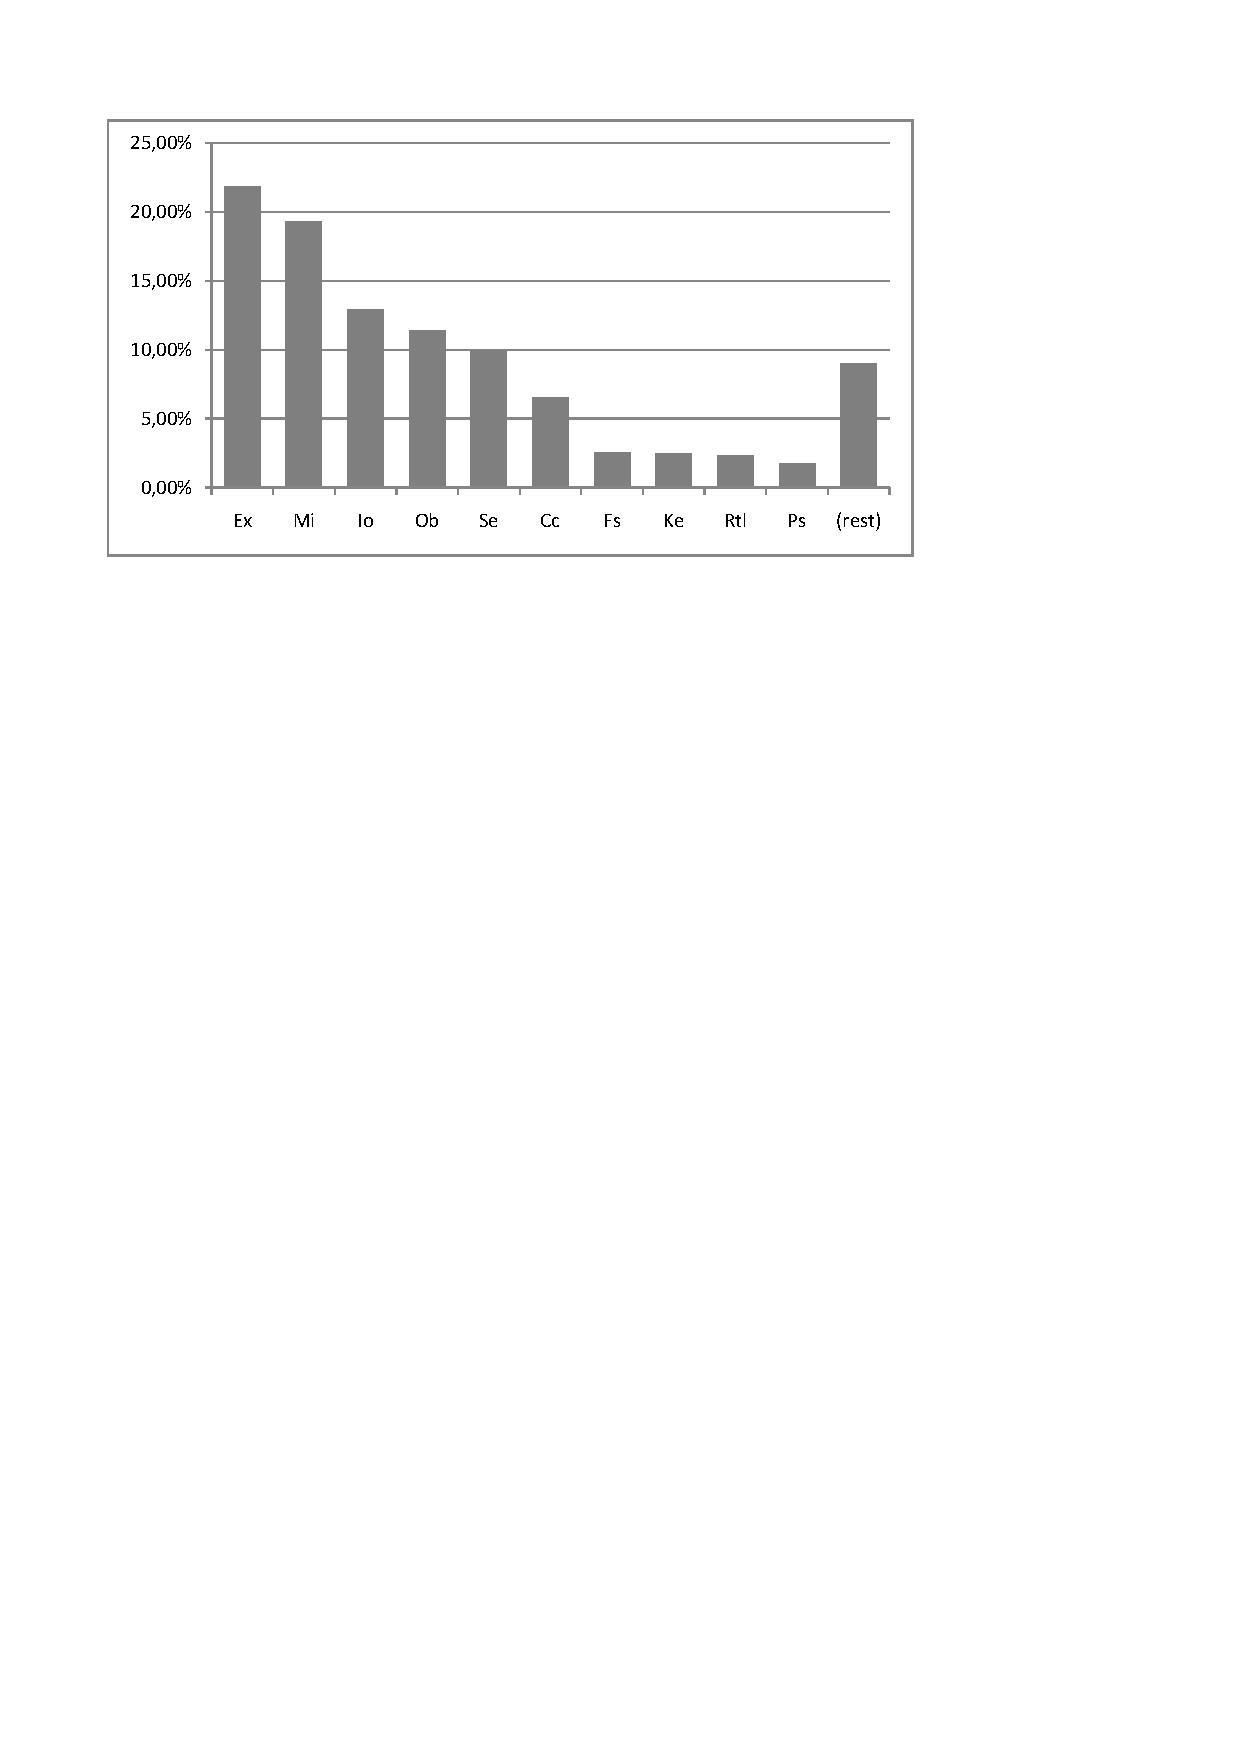
\includegraphics[scale=0.75, clip=true, viewport=1.8cm 20cm 17cm 28cm]{images/diagrams/HistogramSingleBuild.pdf} 
\caption{Distribution of traced routines for a single WRK build} 
\label{HistogramSingleBuild} 
\end{centering} 
\end{figure}


\subsection{System}
All test runs have been performed on a Windows Server 2003 SP2 system, using a retail
kernel (free build). The system has been equipped with an Intel Core 2 Quad Q6600 2.4 GHz 
Quad-Core Processor, 2 GB of RAM and a single 465 GB SATA hard disk. 
In order to discern tracing-related disk accesses 
from other disk accesses, a dedicated hard disk partition has been used for storing the trace 
files. 

The system ran without kernel debugger attached and Driver Verifier disabled for all drivers.
After each test run, the system was rebooted. For the tracing solution itself, the free 
build, i.e. a non-debug, optimized build was used for all tests. Finally, a total of 512 
buffers, each roughly 256 KB in size, has been used for the internal buffer management.

\subsection{Performance Counters}
In order to observe the test runs in more detail, performance counters were used. The
FBT Layer DLL has been augmented to serve as a performance counter DLL, retrieving performance
data from the FBT Agent. The supported performance counters are:

\begin{compactitem}
	\item Instrumented Routines Count: The current number of instrumented routines.
	\item Buffers (Free): Number of free event data buffers in pool.
	\item Buffers (Dirty): Number of dirty event data buffers waiting to be flushed to disk.
	\item Buffers (Collected): Number of event data buffers written to disk.
	\item Prealloc. Pool (Free): Number of free preallocated ThreadData structures.
	\item Prealloc. Pool (Failed Allocations): Failed allocations from the ThreadData preallocated pool.
	\item Reentrant executions (Delta): Number of times an event could not be captured because
				of reentrance (See chapter \ref{sec:ThunkReentrance})
	\item Events dropped (Entry, Delta): Dropped entry events because of buffer depletion.
	\item Events dropped (Exit, Delta): Dropped exit events because of buffer depletion.
	\item Events dropped (Unwind, Delta): Dropped exception unwind events because of buffer depletion.
	\item Image Infos dropped (Delta): Dropped image information chunks because of buffer depletion.
	\item Failed chunk flushes (Delta): Number of `chunks', i.e. packets of trace data that failed
				to be flushed to disk.
	\item Events captured: Total number of entry, exit, and unwind events captured\footnote{Note that the
				values are exact to multiples of 1000 only. To avoid cache line thrashing, events are counted 
				thread locally. Not before 1000 events have been captured on a given thread is the global 
				counter updated. Therefore, the last three digits of the global counter value are always zero.}.
	\item Events captured (Delta): Entry, exit, and unwind events captured during last sampling interval.
	\item Exception unwindings: Total number of auxiliary stack unwindings. See chapter \ref{sec:Unwinding}.
	\item Thread Tear downs: Number of threads having exited, requiring a ThreadData tear down.
\end{compactitem}

The FBT Agent delivers absolute figures only. All delta values are calculated by the performance
counter infrastructure based on these absolute figures.

\begin{figure}[htbp] 
\begin{centering} 
%  (x, y), (x, y) from lower left corner
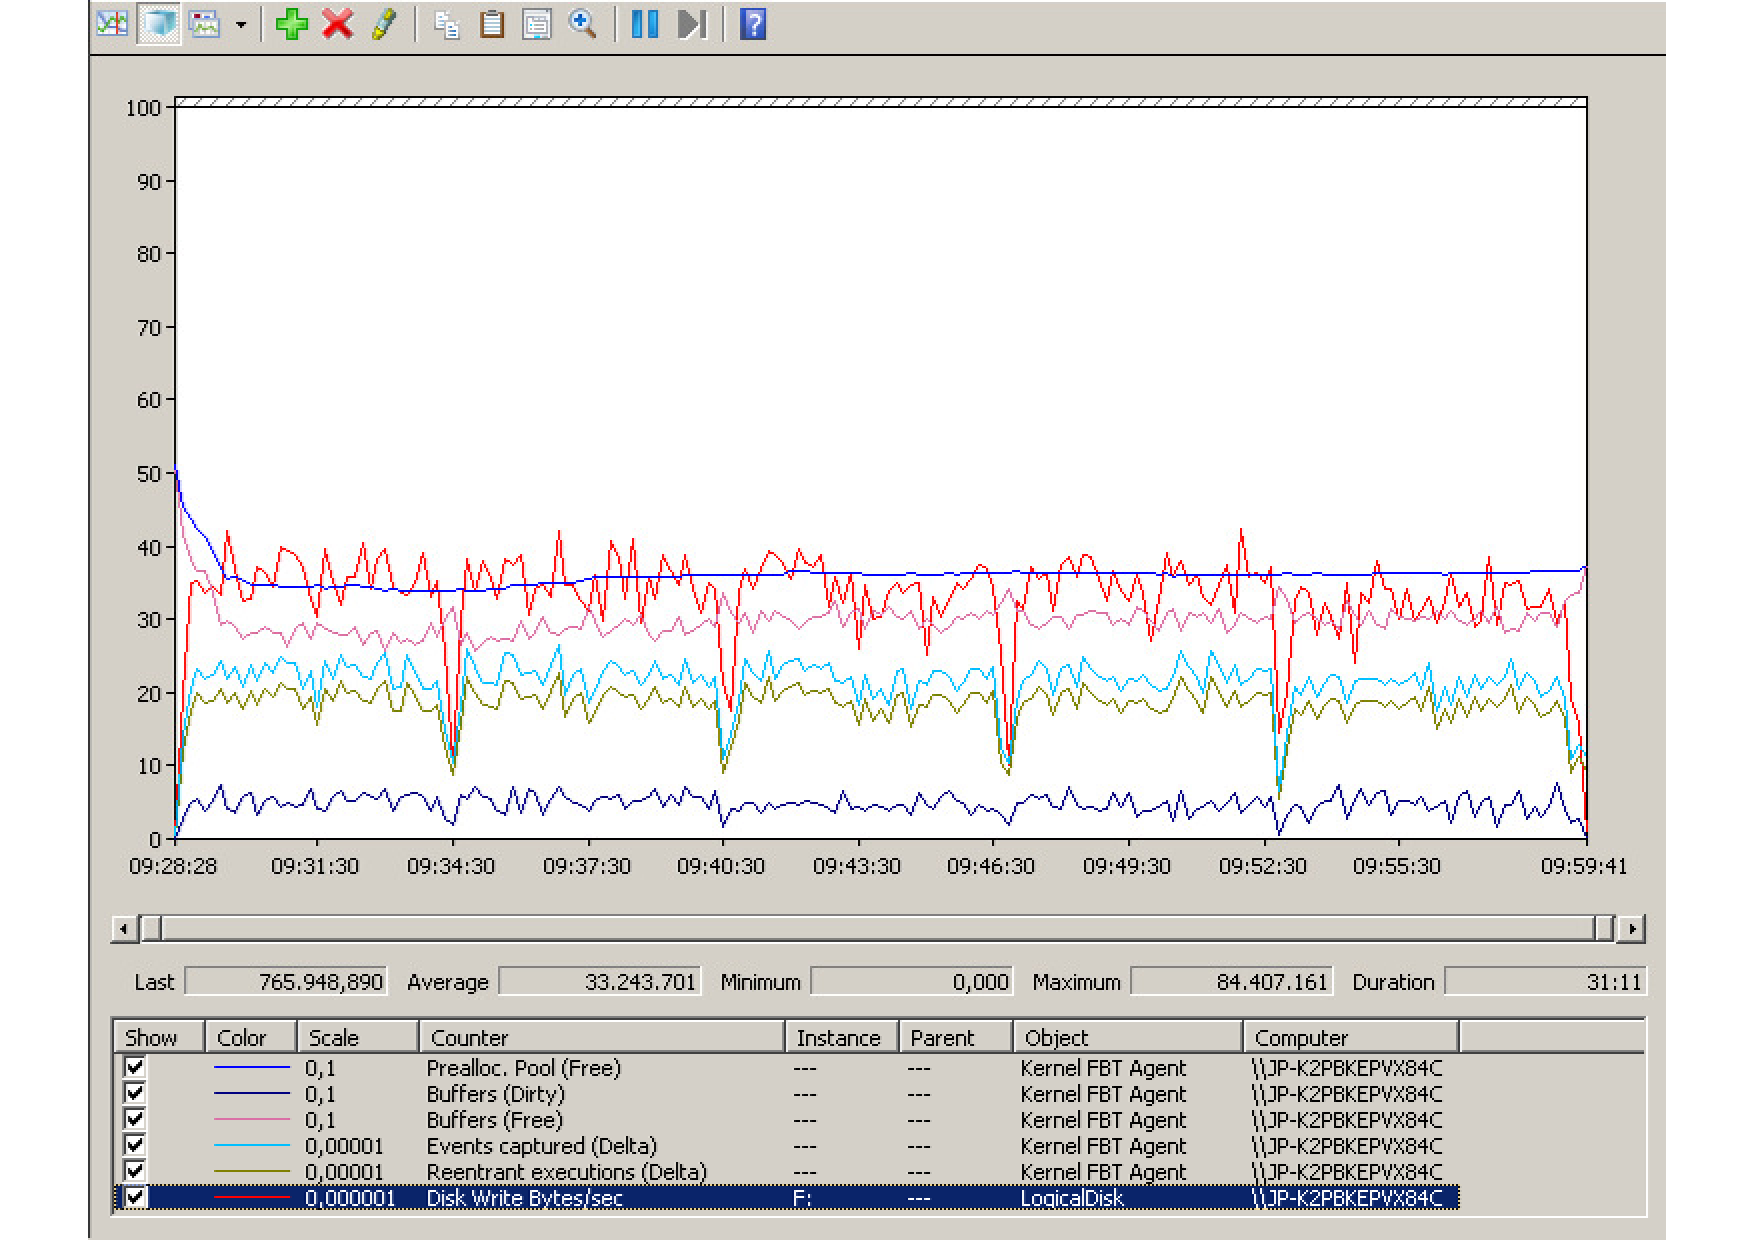
\includegraphics[scale=0.5]{images/PerfmonRun.pdf} 
\caption[Performance Monitor showing selected performance counters]{Performance Monitor showing selected performance counters from a test run comprising five WRK builds with instrumentation on nt!* (i.e. full instrumentation)} 
\label{PerfmonRun} 
\end{centering} 
\end{figure}

Figure \ref{PerfmonRun} shows an example screen shot of the Windows 
\emph{Performance Monitor} displaying data from one of the recorded counter logs. 

%Without going into detail, it is already noticable that the counters
%expose decently low variability during each of the five builds. The values will be discussed in more detail
%in the following sections.

All these performance counters, along with the Windows-provided counters 
\emph{Logical Disk$\backslash$Disk Write Bytes/sec} (for the partition containing the trace file) and \emph{Processor$\backslash$\% Processor Time} have been collected for all testruns using a 
\emph{Counter Log} with a sampling interval of 1 second.

As retrieving the counter data from the FBT agent involves additional I/O processing 
that may influence the overall results, all counters have also been recorded for the 
baseline measurements.

The process of managing performance counters and instrumentation as well as starting the 
build job and measuring elapsed time has been automated in order to avoid unnecessary impact 
of manual intervention. Still, due to the existence of other processes and numerous background 
tasks on a Windows system, the results must be expected to reproducible to a certain degree only.

Concurrently running processes such as services must be expected to routinely perform system calls as well. 
Such system calls, however, may invoke instrumented routines and may thus impact the performance 
counter statistics. Given that the timing behavior of the various processes is unknown, their
behavior must be expected to vary among different test runs. As a result, the exact performance
counter results must be expected to vary as well. Still, this impact is assumed to be of minor 
significance and is thus ignored in the following discussion.

\subsection{Test runs}
Three types of test runs have been conducted:

\begin{itemize}
	\item	Kernel, capturing only: The kernel image has been instrumented to various degrees and
				the events have been captured. Once captured, however, the events were dropped immediately.
				That is, events have not been written to a buffer and have not been written to disk. The results
				from this run therefore show how much overhead the capturing itself introduces.
	\item Kernel, with writing to disk. Again, the kernel image has been instrumented to various 
				degrees. Events were handled by the buffer management and finally written to disk. The
				results from this run therefore show the overall overhead of both capturing and persisting
				the event data. 
	\item Driver, with writing to disk. Not the kernel, but a driver has been instrumented. Having
				chosen ntfs.sys, the driver implementing the NTFS file system, as target, the rationale 
				behind this test run is merely to show that 
				certain drivers may yield substantially different figures, especially with regard to
				exception unwinding.
\end{itemize}

Handling and writing event data to disk clearly imposes additional overhead, so that the
total overhead in the respective test runs will necessarily be higher. There is, however,
an additional point to notice: The code used to perform the task of writing event data to disk 
itself makes use of kernel routines such as those of the I/O manager. In some test runs, these 
routines have been instrumented, so that writing events to disk generates additional events.
Handling these additional events, however, will again increase the workload and lead to 
a higher total overhead.

In those test runs where event data is flushed to disk, the buffer management system discussed
in section \ref{sec:BufferImplementation} is used. Due to its asynchronous nature and its,
albeit limited and \emph{lock-free}, synchronized use of globally shared resources, a slightly 
increased degree of variability and non-determinism should also be expected in the runtime behavior 
and timing measurement results. 

To observe the behavior of the system for different degrees of instrumentation, ten sets of routines 
to be instrumented have been compiled. However, as not the sheer number of routines instrumented
but rather the number of events generated is significant for performance measurements, these sets 
have not been chosen based on their size but on the anticipated number of events generated.

The first set contains all instrumentable routines of the kernel image. Based on the number of events 
generated by a WRK build using this instrumentation set, and taking the distribution among routine
prefixes illustrated in figure \ref{HistogramSingleBuild} into account, nine additional routine sets 
have been defined. Comprising only a subset of the instrumentable routines, each set has been chosen
so that it roughly generates a certain fraction of the maximum number of events. Table \ref{InstrumentationSets}
lists these sets, along with their estimated percentage of events generated in relation to full 
instrumentation.

\begin{table}[h] 
\caption{Instrumentation Sets}
\label{InstrumentationSets}
\centering          
\begin{tabular}{l l l l}    
\hline\hline 
Name & Set (Prefixes) 	& Estimated output 	& Number of 			\\
			&					& (relative to full & routines 			 	\\
			&					& instrumentation)  & 	\\
\hline
S$_{0} (baseline)$ & (none)	&	0\%	&	0		\\
S$_{10}$ & Se	&	10\%	&	182		\\
S$_{20}$ & Io	&	20\%	&	685		\\
S$_{30}$ & Io, Ob	&	30\%	&	813		\\
S$_{40}$ & Ex, Mi	&	40\%	&	681		\\
S$_{50}$ & Ex, Mi, Ob	&	50\%	&	809		\\
S$_{60}$ & Ex, Mi, Io	&	60\%	&	1365		\\
S$_{70}$ & Ex, Mi, Io, Se	&	70\%	&	1546		\\
S$_{80}$ & Ex, Mi, Io, Se, Ob	&	80\%	&	1674	\\
S$_{90}$ & Ex, Mi, Io, Se, Ob, Fs, Cc	&	90\%	&	1995	\\
S$_{100}$ & *	&	100\%	&	5131		\\
\hline
\end{tabular}
\end{table}
%\footnotetext[1]{Relative to the total number of 6990 routines. This number has been counted using the IDA Pro disassembler. The reason that the column does not reach 100\% is that certain routines, as indicated before, are not suited for proper instrumentation.}

\subsection{Results}

The following three tables show the raw results of the test runs performed. 

\begin{table}[h] 
\footnotesize
\addtolength{\tabcolsep}{-2pt}
\caption{Measurements: Kernel, capturing only}
\label{MeasurementsKernelCapturing}
\centering          

\begin{tabular}{l r r r r r r r r r r}    
\hline\hline 
Set				&	Time 		&	Trace &	Events/sec	&Events total	&	Thread 		&	Excep. 	&	Reentran-	&	Logical		 \\
					& [ms]		& size & (non					&(non 				&	tear-			& Un-			& cies			& Disk	 \\
					& 				& [MB] & reentrant)		& reentrant)	& downs			&	winds		&						& [KB/sec]				\\
\hline
S$_{0}$   &	397,941	&	0	&	N/A	&	N/A	&	N/A	&	N/A	&	N/A	&	N/A	\\
\hline
S$_{10}$ 	&	442,263	&	N/A	&	899,254	&	398,381,000	&	1,611	&	0	&	4	&	N/A		\\
S$_{20}$ 	&	467,365	&	N/A	&	1,359,319	&	636,293,000	&	1,630	&	0	&	978	&	N/A		\\
S$_{30}$ 	&	515,550	&	N/A	&	2,106,662	&	1,087,088,000	&	1,647	&	0	&	516	&	N/A		\\
S$_{40}$ 	&	537,817	&	N/A	&	1,714,889	&	922,708,000	&	1,672	&	0	&	710,437	&	N/A		\\
S$_{50}$ 	&	592,178	&	N/A	&	2,286,698	&	1,356,510,000	&	1,649	&	0	&	932,404	&	N/A		\\
S$_{60}$ 	&	603,683	&	N/A	&	2,487,878	&	1,505,372,000	&	1,625	&	0	&	951,276	&	N/A		\\
S$_{70}$ 	&	669,022	&	N/A	&	2,909,408	&	1,949,586,000	&	1,668	&	0	&	1,176,915	&	N/A		\\
S$_{80}$ 	&	728,015	&	N/A	&	3,288,097	&	2,397,390,000	&	1,671	&	0	&	1,322,195	&	N/A		\\
S$_{90}$ 	&	761,557	&	N/A	&	3,416,100	&	2,607,018,000	&	1,683	&	0	&	1,400,906	&	N/A		\\
S$_{100}$	&	884,868	&	N/A	&	3,290,311	&	2,915,831,000	&	1,703	&	1	&	2,702,529	&	N/A		\\
\hline
\end{tabular}
\end{table}

\begin{table}[h] 
\footnotesize
\addtolength{\tabcolsep}{-2pt}
\caption{Measurements: Kernel, with writing to disk}
\label{MeasurementsKernelWithWriting}
\centering          

\begin{tabular}{l r r r r r r r r r r}    
\hline\hline 
Set				&	Time 		&	Trace &	Events/sec	&Events total	&	Thread 		&	Excep. 	&	Reentran-	&	Logical		 \\
					& [ms]		& size & (non					&(non 				&	tear-			& Un-			& cies			& Disk	 \\
					& 				& [MB] & reentrant)		& reentrant)	& downs			&	winds		&						& [KB/sec]				\\
\hline
S$_{0}$   &	397,941	&	0	&	N/A	&	N/A	&	N/A	&	N/A	&	N/A	&	N/A	\\
\hline
S$_{10}$ 	&	497,419	&	6,143	&	802,811	&	398,423,000	&	1,610	&	0	&	4	&	12,943	\\
S$_{20}$ 	&	660,023	&	10,030	&	994,044	&	651,895,000	&	1,643	&	0	&	53	&	15,900	\\
S$_{30}$ 	&	884,267	&	17,168	&	1,269,215	&	1,115,821,000	&	1,688	&	0	&	454	&	20,297	\\
S$_{40}$ 	&	783,479	&	16,967	&	1,407,650	&	1,100,520,000	&	1,665	&	0	&	603,830	&	70,252	\\
S$_{50}$ 	&	1,064,575	&	25,317	&	1,544,235	&	1,649,048,000	&	1,686	&	0	&	653,136	&	24,703	\\
S$_{60}$ 	&	1,026,918	&	28,464	&	1,869,531	&	1,919,400,000	&	1,695	&	0	&	750,117	&	28,953	\\
S$_{70}$ 	&	1,453,399	&	37,063	&	1,689,525	&	2,418,062,000	&	1,681	&	0	&	712,852	&	26,273	\\
S$_{80}$ 	&	1,648,374	&	45,775	&	1,880,908	&	2,987,434,000	&	1,715	&	0	&	789,757	&	28,368	\\
S$_{90}$ 	&	1,566,561	&	52,347	&	2,181,138	&	3,416,633,000	&	1,677	&	0	&	937,571	&	28,369	\\
S$_{100}$	&	1,869,358	&	60,773	&	2,134,650	&	3,967,796,000	&	1,677	&	0	&	1,824,291	&	33,243	\\
\hline
\end{tabular}
\end{table}

\begin{table}[h] 
\footnotesize
\addtolength{\tabcolsep}{-2pt}
\caption{Measurements: Ntfs.sys, with writing to disk}
\label{MeasurementsNtfsWithWriting}
\centering          

\begin{tabular}{l r r r r r r r r r r}    
\hline\hline 
Set				&	Time 		&	Trace &	Events/sec	&Events total	&	Thread 		&	Excep. 	&	Reentran-	&	Logical		 \\
					& [ms]		& size & (non					&(non 				&	tear-			& Un-			& cies			& Disk	 \\
					& 				& [MB] & reentrant)		& reentrant)	& downs			&	winds		&						& [KB/sec]				\\
\hline
S$_{0}$   &	397,941	&	0	&	N/A	&	N/A	&	N/A	&	N/A	&	N/A	&	N/A	\\
\hline
S$_{100}$	&	1,085,506	&	24,011	&	1,447,219	&	1,589,072,000	&	1,482	&	12,251	&	1,449,883	&	23,045	\\ 
\hline
\end{tabular}
\end{table}


Based on these raw numbers, a number of basic observations can be made:
\begin{itemize}
	\item Although the workload has been the same for all runs, the figure \emph{Thread Tear downs}
				varies slightly. This must be expected to be a result of the existence of background tasks
				and other activity on the system.
	\item Comparing the \emph{Time} and \emph{Events/sec (non reentrant)} figures of table
				\ref{MeasurementsKernelCapturing} with those of table \ref{MeasurementsKernelWithWriting},
				shows that the effort required to handle and write the event data to disk is
				non negligible: Builds take significantly longer and as a consequence, the event rate
				is lower when events are written to disk.
	\item Regarding the number of reentrances, there is a sharp rise between S$_{30}$ and
				S$_{40}$ (see figure \ref{Performance_Reent}). 
				S$_{30}$ includes \verb|nt!Io*| and \verb|nt!Ob*|, S$_{40}$ comprises \verb|nt!Ex*| and \verb|nt!Mi*|. 
				It is the latter set of routines, \verb|nt!Mi*|, that may be expected to be the cause of this
				rise: These routines, part of the Memory Manager, are frequently invoked from within
				trap and interrupt handlers. As such, reentrance is more likely to occur
				in this routine set than it is in other sets.
	\item While exception unwinds are very rare when tracing the kernel itself, ntfs.sys
				obviously makes frequent use of exceptions and unwinds. With more than 10 unwinds 
				per second in average, this also stresses the importance of the tracing system to 
				properly deal with SEH.
\end{itemize}

\begin{figure}[h] 
\begin{centering} 
%  (x, y), (x, y) from lower left corner
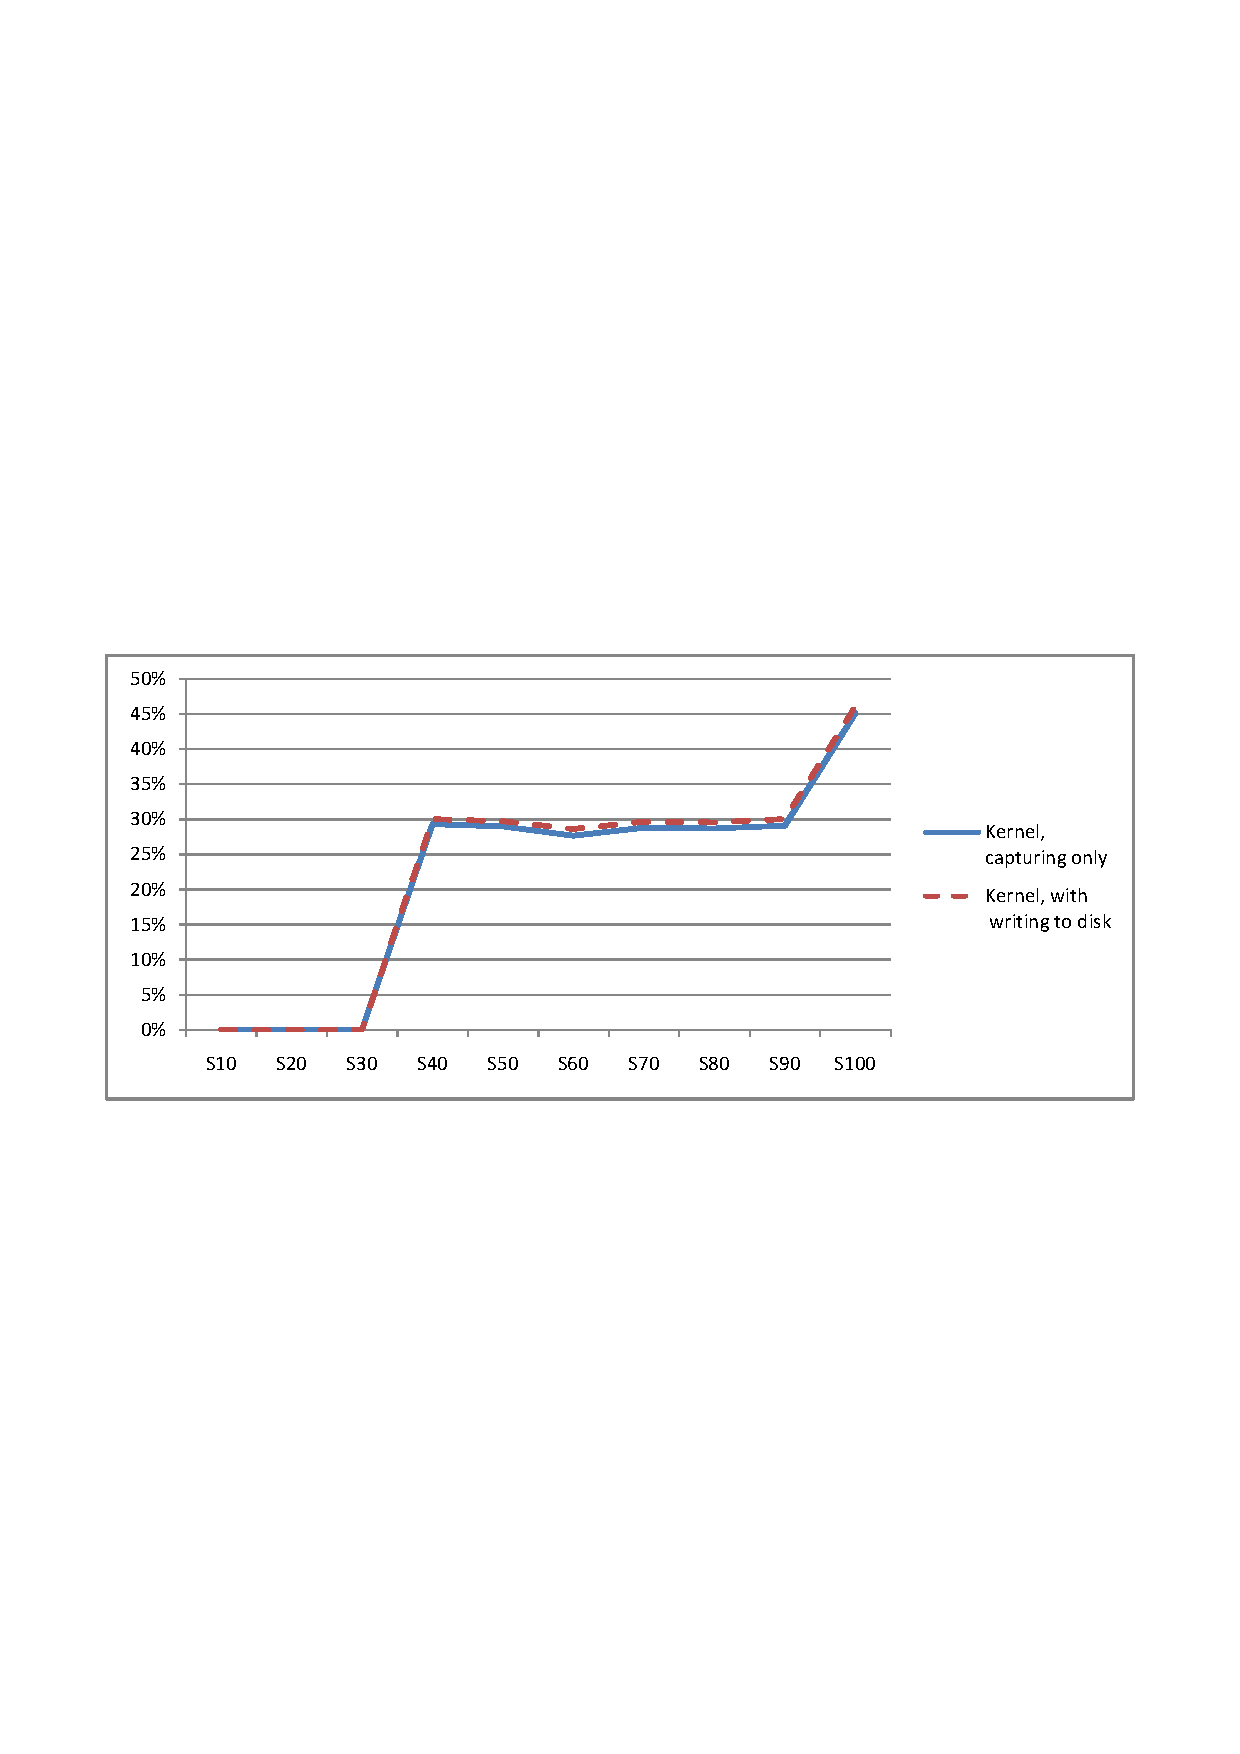
\includegraphics[scale=0.6, clip=true, viewport=1cm 10.5cm 20cm 19cm]{images/diagrams/Performance_Reent.pdf} 
\caption{Percentage of events dropped due to reentrance} 
\label{Performance_Reent} 
\end{centering} 
\end{figure}

By relating the figures obtained by the various test runs with those obtained by the baseline
measurement, it is possible to calculate the overhead imposed by the tracing activity:

\begin{itemize}
	\item \emph{Total Overhead}: Percentage by which the total run time has increased. 
	\item \emph{Overhead/100 M events}: Overhead in relation to the number of events generated, i.e.
				percentage by which the total run time has increased for each 100 million events handled.
				Events dropped due to reentrance are ignored by this figure.
	\item \emph{Avg. Time/event}: Average time value, in nanoseconds, by which the total run time has 
				increased for each event handled. Again, events dropped due to reentrance are ignored by this figure.
\end{itemize}

\begin{table}[h] 
\footnotesize
\addtolength{\tabcolsep}{-2pt}
\label{Overhead}
\caption{Measurements: Overhead}
\centering          

\begin{tabular}{l r r r r r r r}    
\hline\hline 
	&	\multicolumn{3}{c}{Kernel, capturing only} & & \multicolumn{3}{c}{Kernel, with writing to disk} \\
\hline  
	&	Total	&	Overhead/	&	Avg. Time/	&		&	Total	&	Overhead/	&	Avg. Time/	\\
	&	Overhead	&	100 M events	&	event [ns]	&		&	Overhead	&	100 M events	&	event [ns]	\\
\hline
S$_{10}$ &	11.14\%	&	2.80\%	&	111	&		&	25.00\%		&	6.27\%	&	249	\\
S$_{20}$ &	17.45\%	&	2.74\%	&	109	&		&	65.86\%		&	10.10\%	&	402	\\
S$_{30}$ &	29.55\%	&	2.72\%	&	108	&		&	122.21\%	&	10.95\%	&	435	\\
S$_{40}$ &	35.15\%	&	3.81\%	&	151	&		&	96.88\%		&	8.80\%	&	350	\\
S$_{50}$ &	48.81\%	&	3.60\%	&	143	&		&	167.52\%	&	10.16\%	&	404	\\
S$_{60}$ &	51.70\%	&	3.43\%	&	136	&		&	158.06\%	&	8.23\%	&	327	\\
S$_{70}$ &	68.12\%	&	3.49\%	&	139	&		&	265.23\%	&	10.97\%	&	436	\\
S$_{80}$ &	82.95\%	&	3.46\%	&	137	&		&	314.23\%	&	10.52\%	&	418	\\
S$_{90}$ &	91.37\%	&	3.50\%	&	139	&		&	293.67\%	&	8.60\%	&	342	\\
S$_{100}$&	122.36\%&	4.20\%	&	166	&		&	369.76\%	&	9.32\%	&	370	\\\hlinen
\end{tabular}
\end{table}

\begin{figure}[h] 
\begin{centering} 
%  (x, y), (x, y) from lower left corner
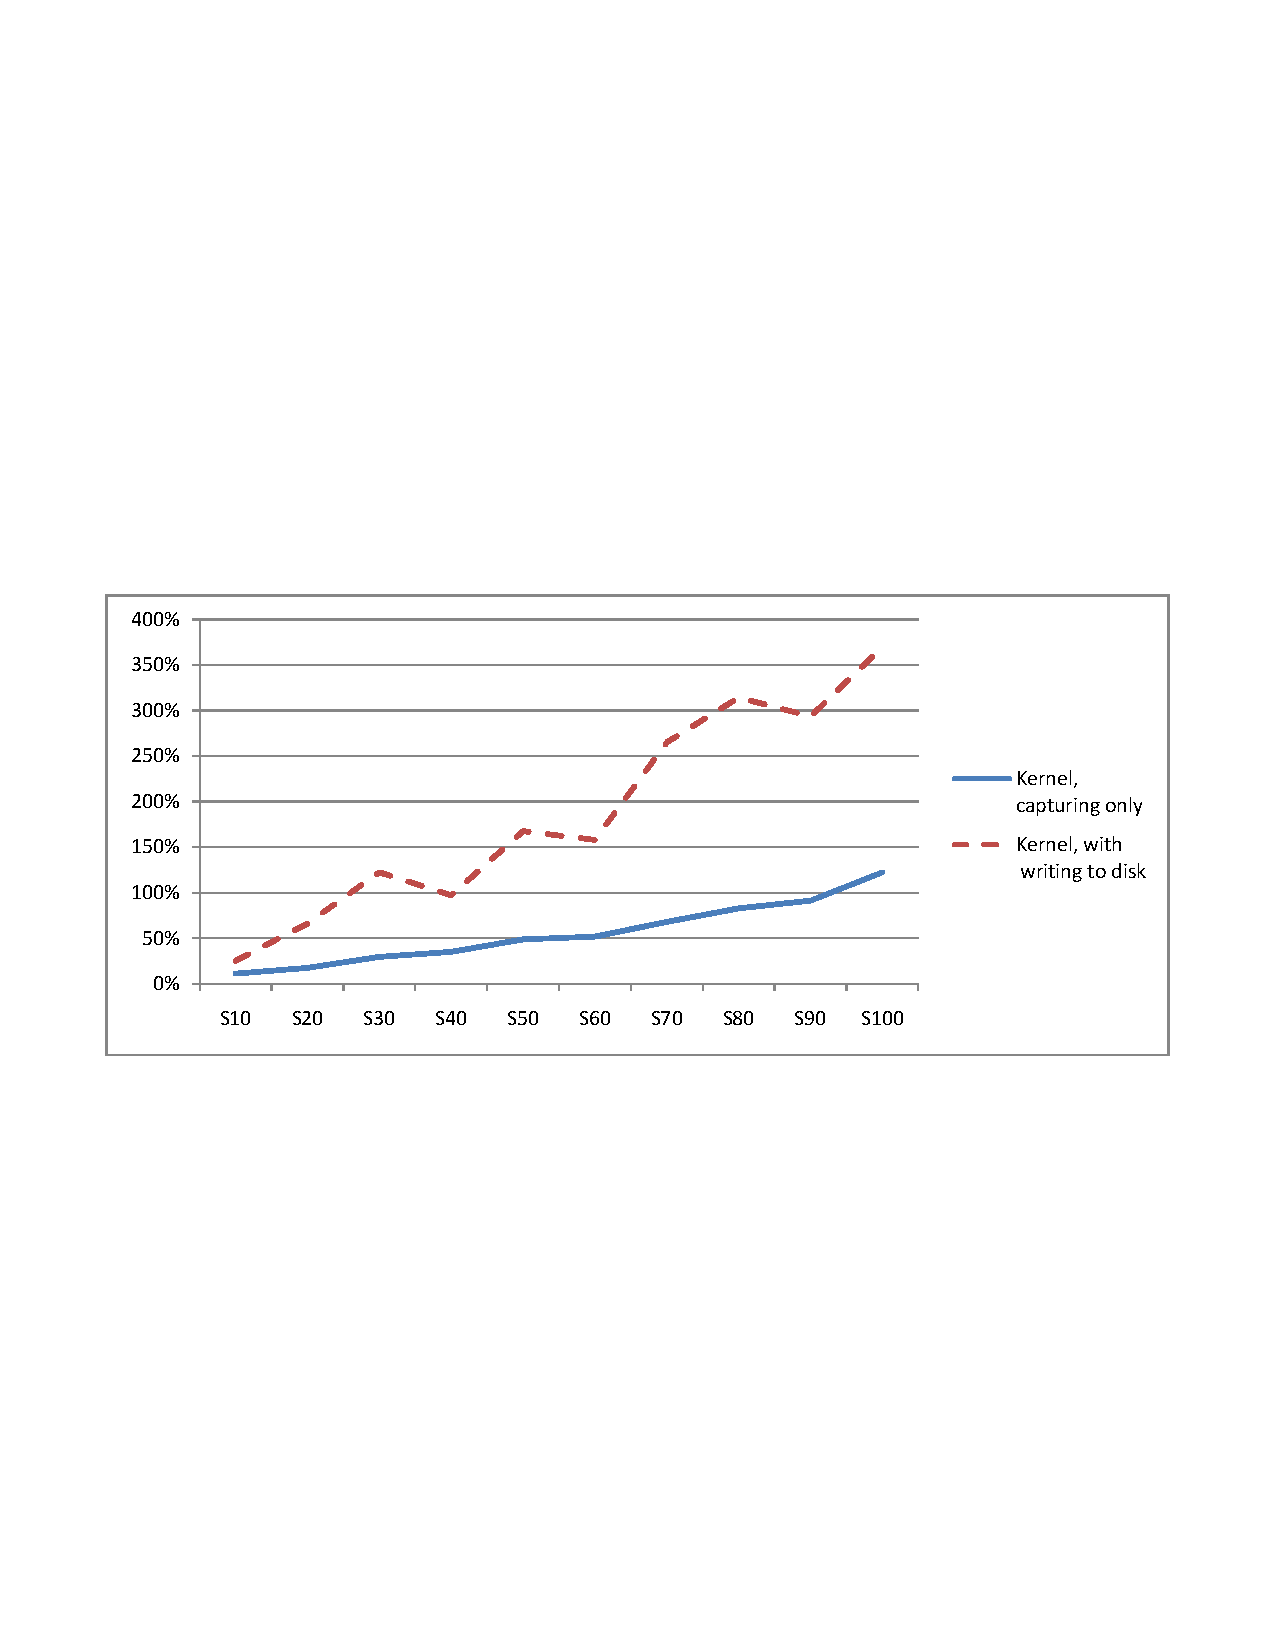
\includegraphics[scale=0.6, clip=true, viewport=1cm 10cm 20cm 19cm]{images/diagrams/Performance_TotalOverhead.pdf} 
\caption{Total Overhead} 
\label{Performance_TotalOverhead} 
\end{centering} 
\end{figure}

\begin{figure}[h] 
\begin{centering} 
%  (x, y), (x, y) from lower left corner
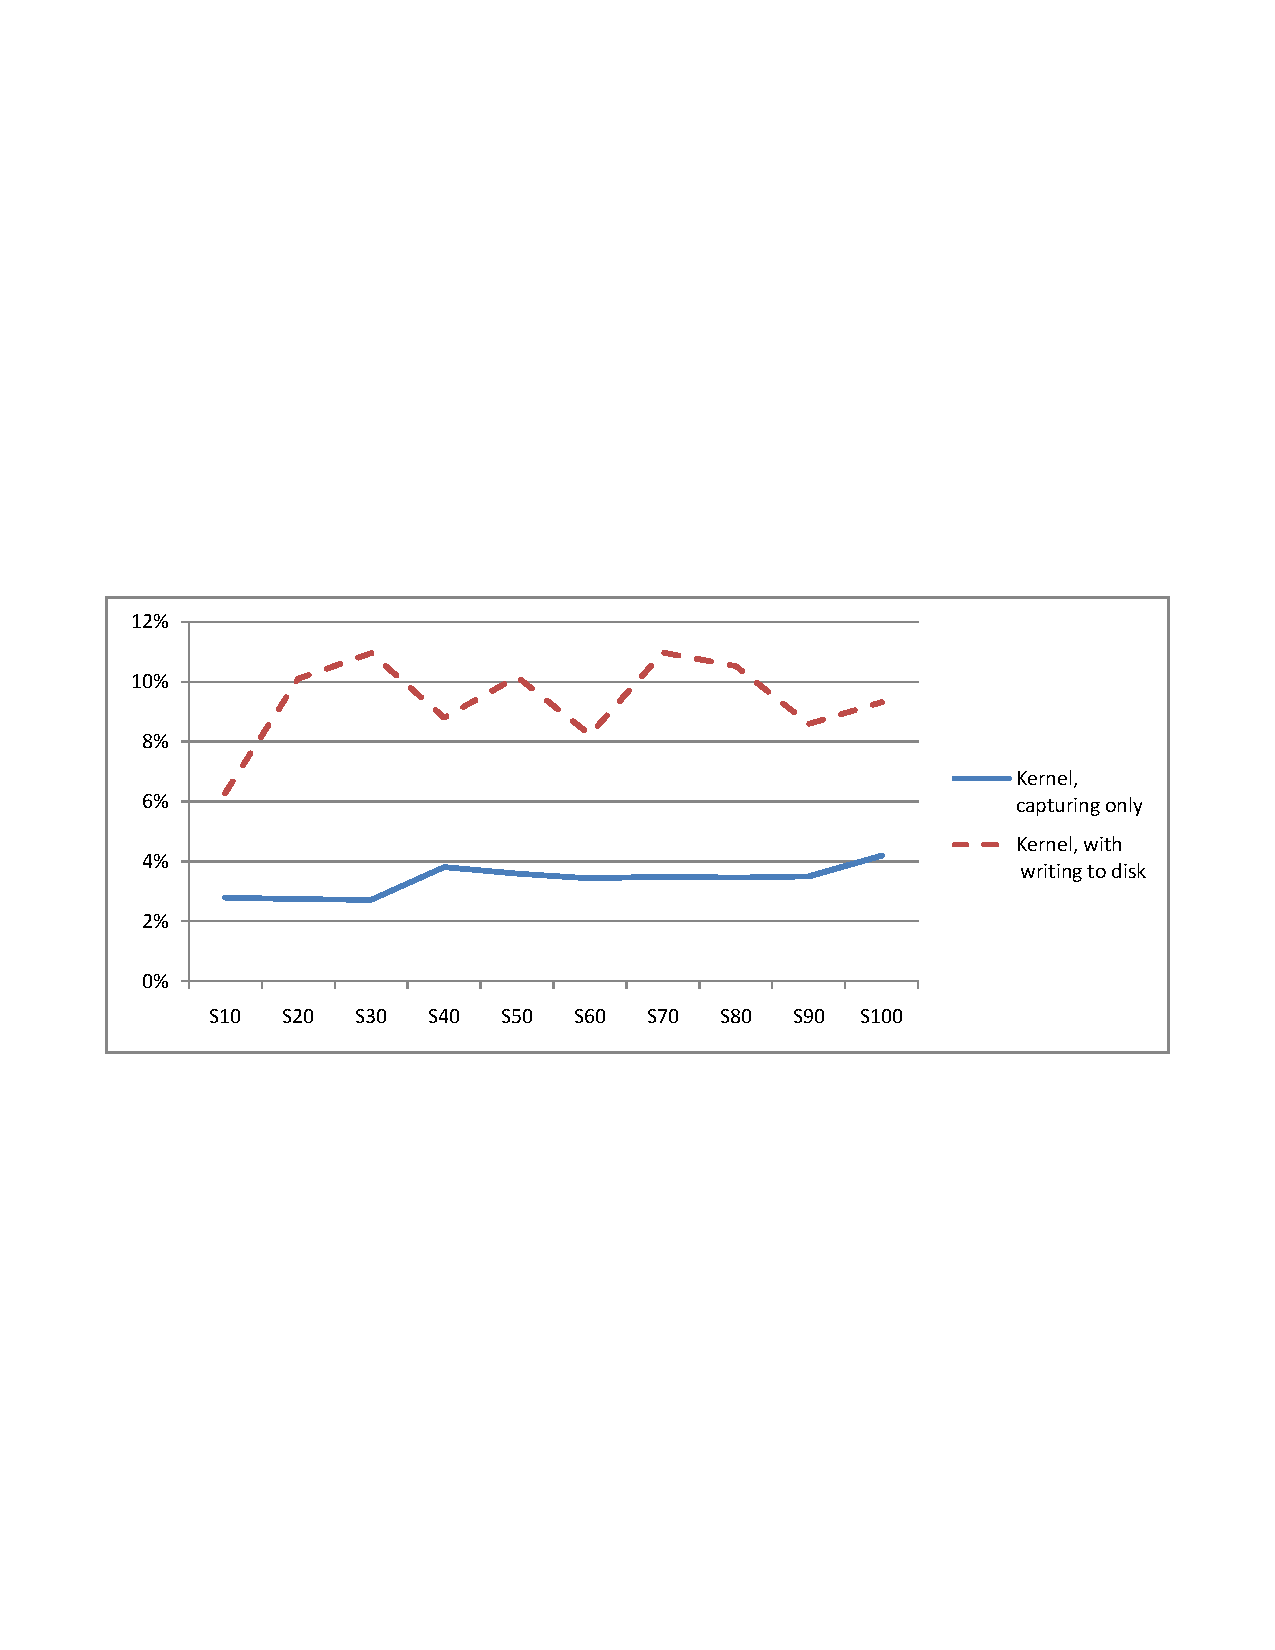
\includegraphics[scale=0.6, clip=true, viewport=1cm 10cm 20cm 19cm]{images/diagrams/Performance_100M.pdf} 
\caption{Overhead for each 100 million events handled} 
\label{Performance_100M} 
\end{centering} 
\end{figure}

\begin{figure}[h] 
\begin{centering} 
%  (x, y), (x, y) from lower left corner
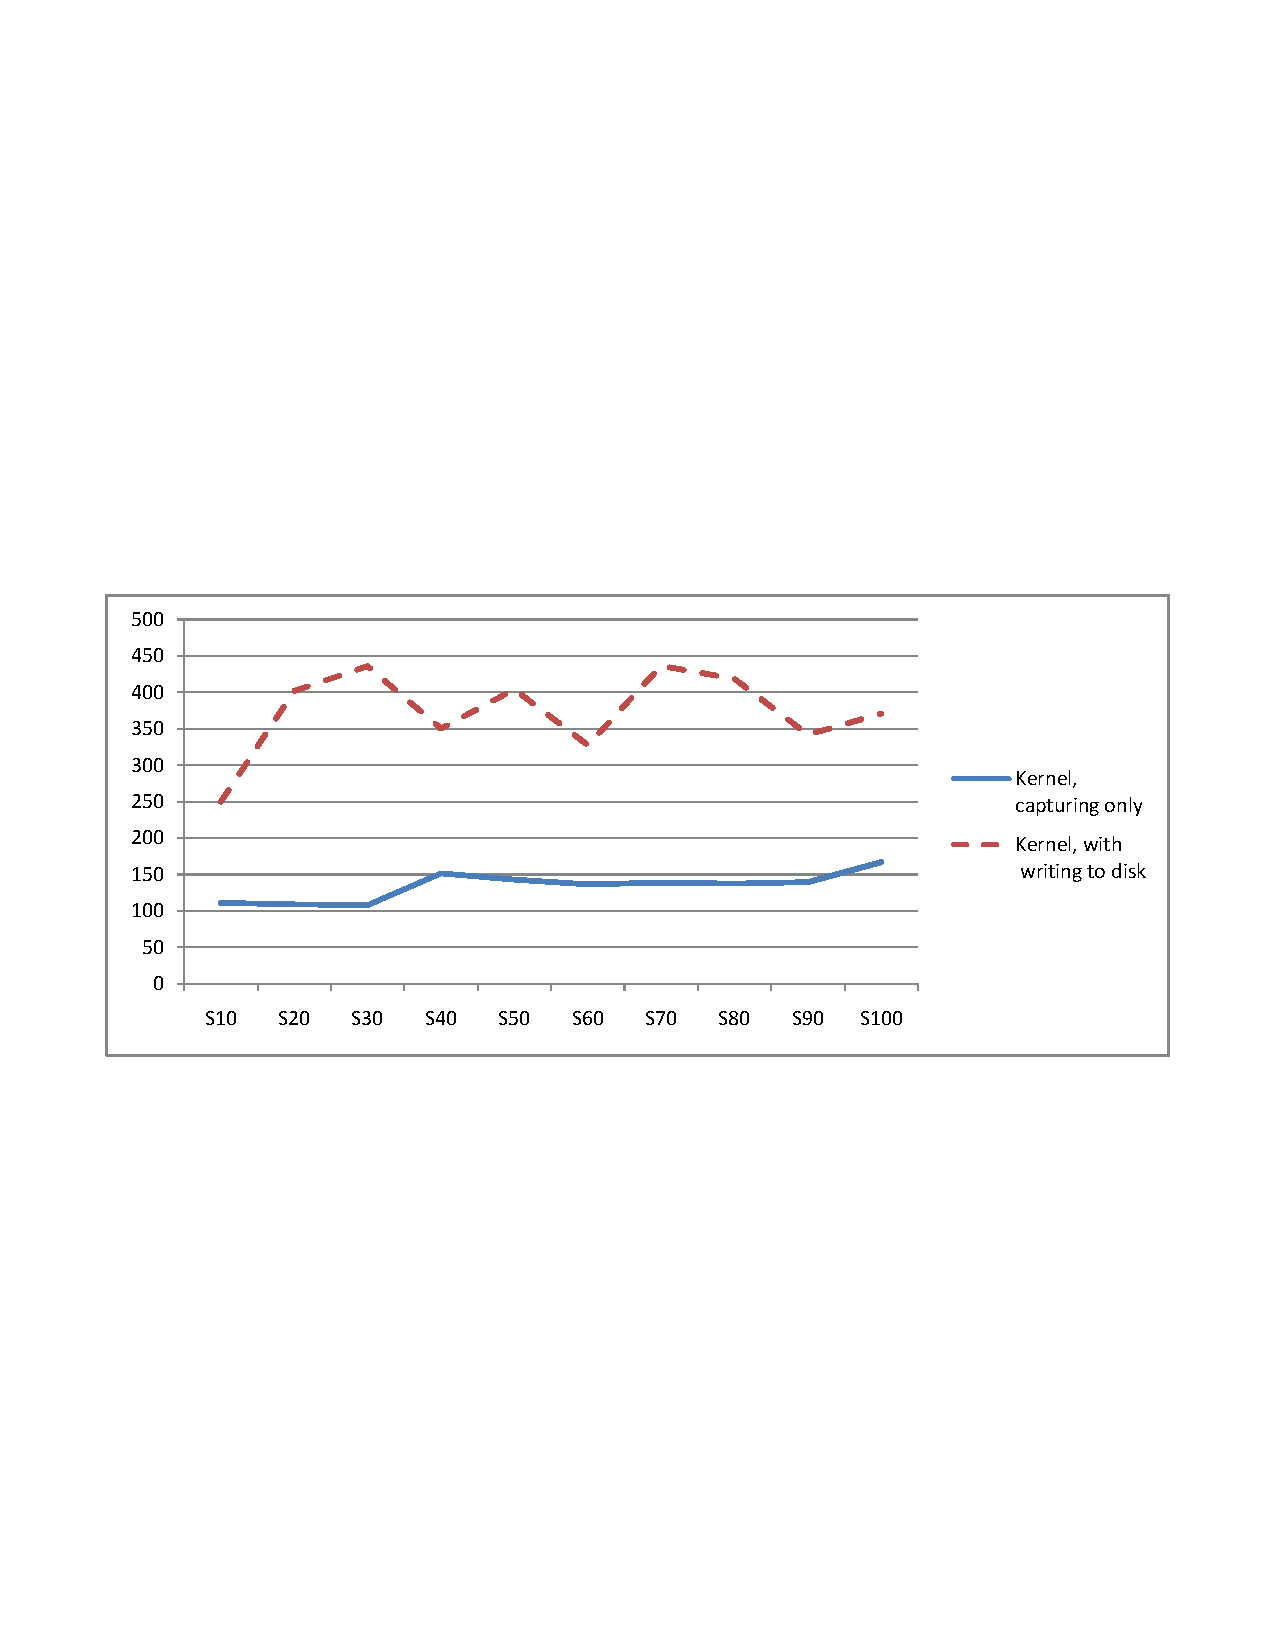
\includegraphics[scale=0.6, clip=true, viewport=1cm 10cm 20cm 19cm]{images/diagrams/Performance_Avg.pdf} 
\caption{Average overhead for each event handled, in nanoseconds} 
\label{Performance_Avg} 
\end{centering} 
\end{figure}

%\begin{table}[h] 
%\footnotesize
%\addtolength{\tabcolsep}{-2pt}
%\label{OverheadPer1Mevps}
%\caption{Measurements: Overhead per 1 M events/sec}
%\centering          
%\begin{tabular}{l l l l l l}    
%\hline\hline 
%	&	\multicolumn{2}{c}{Kernel, capturing only} & & \multicolumn{2}{c}{Kernel, with writing to disk} \\
%\hline  
%	&	non reentrant	&	incl. reentrant	&		&	non reentrant	&	incl. reentrant	\\
%\hline
%S$_{10}$ 	&	12.39\%	&	12.39\%	&		&	31.14\%	&	31.14\%	\\
%S$_{20}$ 	&	12.83\%	&	12.82\%	&		&	66.25\%	&	66.25\%	\\
%S$_{30}$ 	&	14.03\%	&	14.03\%	&		&	96.29\%	&	96.25\%	\\
%S$_{40}$ 	&	20.50\%	&	14.49\%	&		&	68.83\%	&	48.17\%	\\
%S$_{50}$ 	&	21.35\%	&	15.16\%	&		&	108.48\%	&	76.24\%	\\
%S$_{60}$ 	&	20.78\%	&	15.03\%	&		&	84.54\%	&	60.34\%	\\
%S$_{70}$ 	&	23.41\%	&	16.67\%	&		&	156.98\%	&	110.40\%	\\
%S$_{80}$ 	&	25.23\%	&	17.99\%	&		&	167.06\%	&	117.66\%	\\
%S$_{90}$ 	&	26.75\%	&	18.97\%	&		&	134.64\%	&	94.16\%	\\
%S$_{100}$	&	37.19\%	&	20.42\%	&		&	173.22\%	&	93.40\%	\\
%\hline
%\end{tabular}
%\end{table}
%
%
%\begin{figure}[h] 
%\begin{centering} 
%%  (x, y), (x, y) from lower left corner
%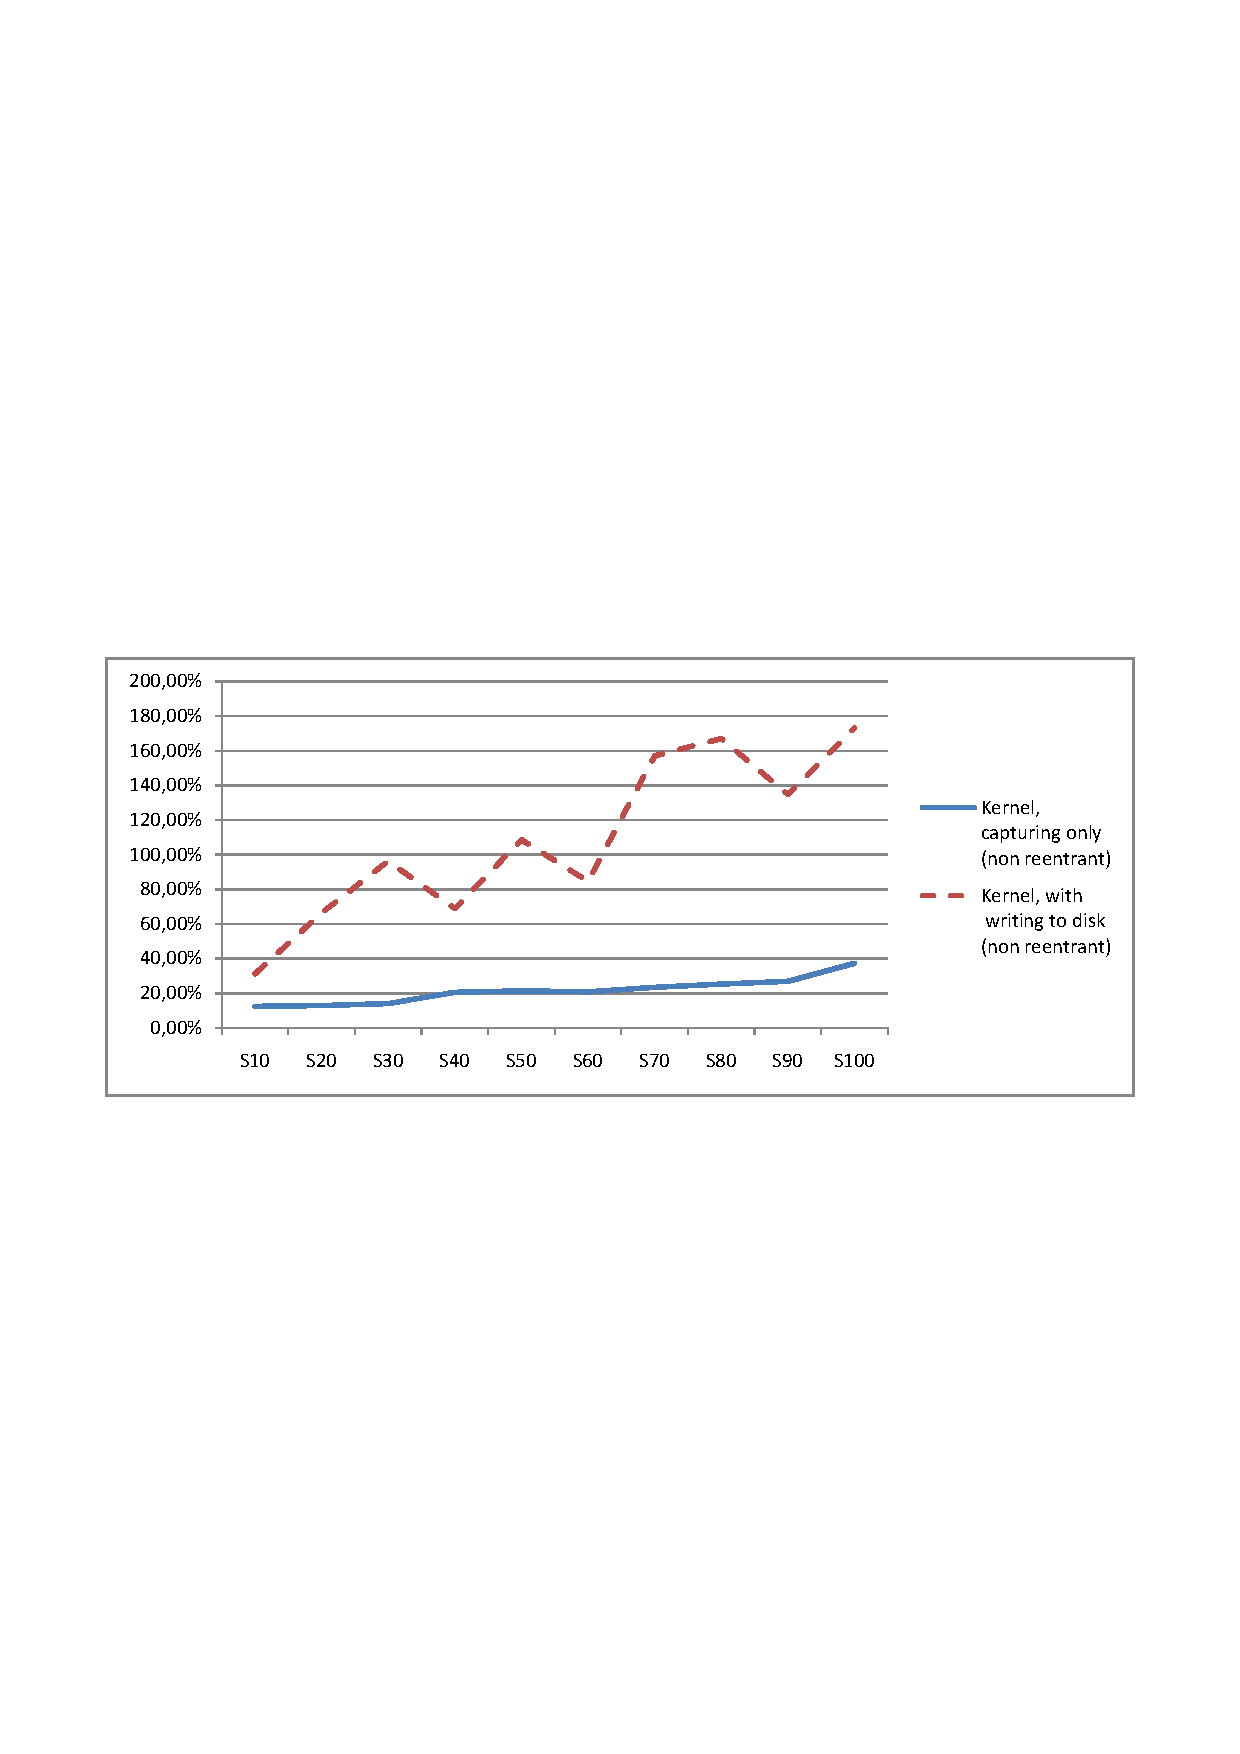
\includegraphics[scale=0.6, clip=true, viewport=1cm 10cm 20cm 19cm]{images/diagrams/Performance_1Meps.pdf} 
%\caption{Average overhead imposed by 1 million events captured per second} 
%\label{Performance_1Meps} 
%\end{centering} 
%\end{figure}


Figure \ref{Performance_TotalOverhead} shows the \emph{Total Overhead} in relation to 
different routine sets. With full instrumentation on the kernel image, the build process
slows down by roughly 122\%. When the event data is also flushed to disk, the overhead 
increases to 369\%.

The fact that the overhead rises with an increasing number of events handled certainly 
does not come at a surprise. Yet, it is notable that the overhead evolves gracefully, 
i.e. almost linearly. The diagram also underlines what has been indicated before -- 
that those measurements involving writing event data to disk show higher variability.

However, figure \ref{Performance_TotalOverhead} does not yet express in how far the overhead
of handling a single event is dependent on the total number of events captured. For the 
solution to be \emph{scalable}, it is crucial that the overhead evolves gracefully when
the total number of events increases. That is, the overhead per event should not rise
significantly.

The diagrams \ref{Performance_100M} and \ref{Performance_Avg} show how the overhead
per event evolves. With an increasing number of total events captured, the overhead per single event
indeed increases, yet only slightly.

%A similar picture is painted by table \ref{OverheadPer1Mevps} and figure 
%\ref{Performance_1Meps}, which assess the overhead from a slightly different angle, and
%list the relative overhead caused by each \emph{1 million events captured per second}. 


To explain this rise, it is important to notice that the events dropped due
to reentrance impose an overhead, yet are not regarded by these numbers. In fact, comparing
the respective graphs of these two figures with the those of figure \ref{Performance_Reent}, there is a
remarkable similarity to be noticed: Between S$_{30}$ and S$_{40}$ as well as between
S$_{90}$ and S$_{100}$, there is a steep incline in all graphs. 

To yield more exact figures, the overhead imposed by events that have been dropped due
to reentrace would need to be factored in. This, however, is problematic to achieve as 
the overhead imposed by a reentrant event is less than the overhead of a properly captured 
event. Nonetheless, it is safe to assume that the rise is at least partially caused by reentrance. 

Finally, although less smooth, the graphs illustrating the overhead when events are additionally 
written to disk evolve gracefully in all diagrams as well. This may be interpreted as an indication for that
the buffer management and disk flushing activity does not suffer from any serious
performance bottlenecks.



\chapter{Conclusion}
Dynamic function boundary tracing of kernel mode components has many potential applications, 
yet its potentials have largely been dormant on the Windows NT platform.

This thesis has presented an overview and has proposed a classification scheme covering
techniques that may be used for implementing such tracing systems. With the creation
of NTrace, we demonstrated that implementing such a tracing system for Windows NT
is in fact technically feasible.

In addition to that, we have shown that it is possible for a tracing system to integrate
with Windows Structured Exception Handling. Besides allowing the system to attain exception
safety, such integration also adds significant value to the tracing results as it allows exception unwinds, 
like function entry and exit events, to be properly traced.

Utilizing synergy effects with the Microsoft Hotpatching infrastructure, NTrace also
has shown that the challenges of runtime code modification can be successfully overcome. 

Although the exact requirements on a tracing solution vary with the individual purpose, 
the general aims of creating a system that is detailed, frugal, and scalable could hence be achieved.

\section*{Limitations and Outlook}
The focus of NTrace has clearly lied on capturing trace information while maintaining 
reasonable performance. As such, the system should primarily be seen as providing the foundation 
for tools offering features going beyond mere recording of trace information.
Such features could include the ability to filter events -- such as by limiting the 
capturing to certain threads only -- as well as the capability to record parameter
information. Other tools, such as profilers, are equally conceivable.

%The overall applicability of an NTrace-based tool could be further improved by 
%features such as the ability to filter trace events. Currently, all calls to instrumented
%routines, regardless of the thread context, are recorded. Being able to limit recording to
%a selected set of processes or threads could help limiting the overhead and yielding more
%concise results. Moreover, leveraging symbol information to properly record parameter values 
%of routine calls couly also imrove the usefulness of traces.

But there certainly are also aspects to the current implementation of NTrace that leave room to improvement.
Currently, the most important limitation can be seen in the relatively high loss rate of events
due to reentrace. While the current implementation has proven to be able to avoid reentrace-caused
hazards, the \emph{window} of instructions of the CallProxy and EntryThunk in which reentrace 
leads to events being dropped is still larger than necessary. By optimizing and restructuring the respective
assembly code, however, the author expects that the drop rate should be able to be 
lowered significantly.

Much of the implementation of NTrace is both workable in kernel and in user mode. In fact, the 
entire FBT core library has been implemented and tested for either mode. As such, creating the additional
tool support to add the capability to trace user mode processes seems highly auspicious in order
to increase the potential fields of application for NTrace.

Finally, NTrace is currently limited to the IA-32 architecture. Although a non-negligible part of
the implementation -- such as instrumentation and exception handling -- is architecture-specific,
porting NTrace to AMD64 seems viable, albeit not trivial. Notwithstanding their common heritage,
AMD64 poses different challenges on such an implementation. For instance, while 
being slightly more forgiving with regard 
to runtime code modification, the increased address space brings up the issues of jump distances
again. Moreover, leveraging hotpatchable images on AMD64 requires a certain, although limited 
amount of disassembly to be performed at runtime. PatchGuard \cite{Microsoft07}, the facility of AMD64 Windows
kernels to prevent certain code modifications at runtime, poses another challenge to such porting
efforts. That is, NTrace on AMD64 would likely be limited to tracing drivers, while not being 
able to trace the kernel itself as well the system images \emph{hal} and \emph{ndis} \cite{Skywing05}. Still, 
such porting effort could further enlarge the applicability of NTrace.
